%% abtex2-modelo-trabalho-academico.tex, v-1.9.2 laurocesar
%% Copyright 2012-2014 by abnTeX2 group at http://abntex2.googlecode.com/ 
%%
%% This work may be distributed and/or modified under the
%% conditions of the LaTeX Project Public License, either version 1.3
%% of this license or (at your option) any later version.
%% The latest version of this license is in
%%   http://www.latex-project.org/lppl.txt
%% and version 1.3 or later is part of all distributions of LaTeX
%% version 2005/12/01 or later.
%%
%% This work has the LPPL maintenance status `maintained'.
%% 
%% The Current Maintainer of this work is the abnTeX2 team, led
%% by Lauro César Araujo. Further information are available on 
%% http://abntex2.googlecode.com/
%%
%% This work consists of the files abntex2-modelo-trabalho-academico.tex,
%% abntex2-modelo-include-comandos and abntex2-modelo-references.bib
%%

% ------------------------------------------------------------------------
% ------------------------------------------------------------------------
% abnTeX2: Modelo de Trabalho Academico (tese de doutorado, dissertacao de
% mestrado e trabalhos monograficos em geral) em conformidade com 
% ABNT NBR 14724:2011: Informacao e documentacao - Trabalhos academicos -
% Apresentacao
% ------------------------------------------------------------------------
% ------------------------------------------------------------------------

\documentclass[
    oneside, %opção para documentos digitais adicionada por mim
	% -- opções da classe memoir --
	12pt,				% tamanho da fonte
	%openright,			% capítulos começam em pág ímpar (insere página vazia caso preciso)
	%twoside,			% para impressão em verso e anverso. Oposto a oneside
	a4paper,			% tamanho do papel. 
	% -- opções da classe abntex2 --
	chapter=TITLE,		% títulos de capítulos convertidos em letras maiúsculas
	%section=TITLE,		% títulos de seções convertidos em letras maiúsculas
	%subsection=TITLE,	% títulos de subseções convertidos em letras maiúsculas
	%subsubsection=TITLE,% títulos de subsubseções convertidos em letras maiúsculas
	% -- opções do pacote babel --
	english,			% idioma adicional para hifenização
	french,				% idioma adicional para hifenização
	spanish,			% idioma adicional para hifenização
	brazil				% o último idioma é o principal do documento
	]{abntex2}

% ---
% Pacotes básicos 
% ---
\usepackage{libertine}			% Usa a fonte libertine			
\usepackage[T1]{fontenc}		% Selecao de codigos de fonte.
\usepackage[utf8]{inputenc}		% Codificacao do documento (conversão automática dos acentos)
\usepackage{lastpage}			% Usado pela Ficha catalográfica
\usepackage{indentfirst}		% Indenta o primeiro parágrafo de cada seção.
\usepackage{color}				% Controle das cores
\usepackage{graphicx}			% Inclusão de gráficos
\usepackage{microtype} 			% para melhorias de justificação
% ---
		
% ---
% Pacotes adicionais, usados apenas no âmbito do Modelo Canônico do abnteX2
% ---
\usepackage{lipsum}				% para geração de dummy text
% ---

% ---
% Pacotes de citações
% ---
\usepackage[brazilian,hyperpageref]{backref}	 % Paginas com as citações na bibl
\usepackage[alf]{abntex2cite}	% Citações padrão ABNT

%---
% Pacotes adicionados por mim
%---

\usepackage{float}
\usepackage[ruled,vlined]{algorithm2e}
\usepackage{tcolorbox}
\usepackage{amsmath}
\usepackage{subfig}
\usepackage{enumitem}
%\usepackage[section]{placeins}

% --- 
% CONFIGURAÇÕES DE PACOTES
% --- 

% ---
% Configurações do pacote backref
% Usado sem a opção hyperpageref de backref
\renewcommand{\backrefpagesname}{Citado na(s) página(s):~}
% Texto padrão antes do número das páginas
\renewcommand{\backref}{}
% Define os textos da citação
\renewcommand*{\backrefalt}[4]{
	\ifcase #1 %
		Nenhuma citação no texto.%
	\or
		Citado na página #2.%
	\else
		Citado #1 vezes nas páginas #2.%
	\fi}%
% ---

% ---
% Informações de dados para CAPA e FOLHA DE ROSTO
% ---
\titulo{MODELAGEM GEOLÓGICA E AVALIAÇÃO DE INCERTEZA EM MODELOS GEOLÓGICOS USANDO FUNÇÕES DISTÂNCIA ASSINALADAS}
\autor{Roberto Mentzingen Rolo}
\local{Porto Alegre - RS}
\data{2021}
\orientador{João Felipe Coimbra Leite Costa}
%\coorientador{Equipe \abnTeX}
\instituicao{%
  Universidade Federal do Rio Grande do Sul -- UFRGS
  \par
  Escola de Engenharia
  \par
  Programa de Pós-graduação em Engenharia de Minas, Metalúrgica e de Materiais}
\tipotrabalho{Tese (Doutorado)}
% O preambulo deve conter o tipo do trabalho, o objetivo, 
% o nome da instituição e a área de concentração 
\preambulo{Tese submetida ao Programa de Pós-graduação em Engenharia de Minas, Metalúrgica e Materiais (PPGE3M) da Universidade Federal do Rio Grande do Sul como requisito parcial à obtenção do título de Doutor em Engenharia.}
% ---


% ---
% Configurações de aparência do PDF final

% alterando o aspecto da cor azul
\definecolor{blue}{RGB}{41,5,195}

% informações do PDF
\makeatletter
\hypersetup{
     	%pagebackref=true,
		pdftitle={\@title}, 
		pdfauthor={\@author},
    	pdfsubject={\imprimirpreambulo},
	    pdfcreator={LaTeX with abnTeX2},
		pdfkeywords={abnt}{latex}{abntex}{abntex2}{trabalho acadêmico}, 
		colorlinks=true,       		% false: boxed links; true: colored links
    	linkcolor=blue,          	% color of internal links
    	citecolor=blue,        		% color of links to bibliography
    	filecolor=magenta,      		% color of file links
		urlcolor=blue,
		bookmarksdepth=4
}
\makeatother
% --- 

% --- 
% Espaçamentos entre linhas e parágrafos 
% --- 

% O tamanho do parágrafo é dado por:
\setlength{\parindent}{1.3cm}

% Controle do espaçamento entre um parágrafo e outro:
\setlength{\parskip}{0.2cm}  % tente também \onelineskip

% ---
% compila o indice
% ---
\makeindex
% ---

% ----
% Início do documento
% ----
\begin{document}

% Retira espaço extra obsoleto entre as frases.
\frenchspacing 

% ----------------------------------------------------------
% ELEMENTOS PRÉ-TEXTUAIS
% ----------------------------------------------------------
% \pretextual

% ---
% Capa
% ---
\imprimircapa
% ---

% ---
% Folha de rosto
% (o * indica que haverá a ficha bibliográfica)
% ---
\imprimirfolhaderosto*
% ---

% ---
% Inserir a ficha bibliografica
% ---

% Isto é um exemplo de Ficha Catalográfica, ou ``Dados internacionais de
% catalogação-na-publicação''. Você pode utilizar este modelo como referência. 
% Porém, provavelmente a biblioteca da sua universidade lhe fornecerá um PDF
% com a ficha catalográfica definitiva após a defesa do trabalho. Quando estiver
% com o documento, salve-o como PDF no diretório do seu projeto e substitua todo
% o conteúdo de implementação deste arquivo pelo comando abaixo:
%
% \begin{fichacatalografica}
%     \includepdf{fig_ficha_catalografica.pdf}
% \end{fichacatalografica}

% ---
% Inserir folha de aprovação
% ---

% Isto é um exemplo de Folha de aprovação, elemento obrigatório da NBR
% 14724/2011 (seção 4.2.1.3). Você pode utilizar este modelo até a aprovação
% do trabalho. Após isso, substitua todo o conteúdo deste arquivo por uma
% imagem da página assinada pela banca com o comando abaixo:
%
% \includepdf{folhadeaprovacao_final.pdf}
%

% ---
% Agradecimentos
% ---
\begin{agradecimentos}

Agradeço à minha Mãe, às minhas irmãs Todia e Cláudia e meu cunhado Marcelo pelo apoio incondicional. À minha parceira para qualquer tempo Camila. Aos amigos de JF Skeli, Disco, Gunzo, Alves e Dêniel. À república Sparta. Ao meu orientador e grande amigo, Professor João Felipe. Aos colegas de laboratório, principalmente, os parceiros de pesquisa Flávio Amarante e David Drummond. Sem esquecer de outras grandes amizades: Augusto, Marcel, Cristina, Jonas, Luiz, Ryu, Myolo, Ricardinho, Ricardo Colômbia, Kbelo e Anuar. A turma  da programação: Péricles e Átila. Viva o software livre! Agradeço também ao LPM, à Fundação Luiz Englert, à CAPES, à AR2Tech, e ao Governo do Estado do Rio Grande do Sul pelas oportunidades e por incentivarem a conclusão desse doutorado.

\end{agradecimentos}
% ---

% ---
% Epígrafe
% ---
\begin{epigrafe}
    \vspace*{\fill}
	\begin{flushright}
		\textit{"All models are wrong, but some are useful"\\
		George Box}
	\end{flushright}
\end{epigrafe}
% ---

% ---
% RESUMOS
% ---

% resumo em português
\setlength{\absparsep}{18pt} % ajusta o espaçamento dos parágrafos do resumo
\begin{resumo}
    Métodos geoestatísticos para estimativa e simulação de teores de minério requerem a delimitação prévia de domínios estacionários. Apesar da ampla adoção pela indústria de mineração da modelagem implícita com funções de distância assinaladas como alternativa à modelagem explícita para esse fim, os modelos criados dessa forma não avaliam a incerteza sobre a posição real dos contatos geológicos no subsolo. Em muitos casos, a incerteza do modelo geológico pode ser uma fonte de incerteza importante para o projeto e ignorá-la pode ser devastador para o empreendimento. Esta tese propõe e investiga três diferentes metodologias para avaliar a incerteza em modelos geológicos multi-categóricos usando funções de distância assinaladas. Uma das metodologias propostas é baseada em interpolação, enquanto as outras duas são baseadas em simulações Gaussianas não condicionais dentro de uma zona de incerteza. Um estudo de caso foi realizado para cada metodologia. Os resultados foram comparados com a simulação sequencial dos indicadores mostrando que as metodologias propostas podem gerar limites contínuos entre as diferentes litologias do depósito mineral com o realismo geológico esperado. Foram desenvolvidos softwares implementando as metodologias propostas que apresentam um alto nível de automação.

 \textbf{Palavras-chaves}: Modelagem geológica. Modelagem geológica implícita. Avaliação de incerteza. Simulação de contatos geológicos.
\end{resumo}

% resumo em inglês
\begin{resumo}[Abstract]
 \begin{otherlanguage*}{english}
   Geostatistical methods for estimation and simulation of ore grades require the previous delimitation of stationary domains. Despite the widespread adoption by the mining industry of implicit modeling with signed distance functions as an alternative to explicit modeling for this purpose, models created in this way do not assess uncertainty about the real position of the geological contacts in the subsurface. In many cases, the uncertainty of the geological model can be a source of important project uncertainty, and ignoring it can be devastating for the enterprise. This thesis proposes and investigates three different methodologies for assessing uncertainty in multi-categorical geological models using signed distance functions. One of the proposed methodologies is based on interpolation, while the other two are based on unconditional Gaussian simulations inside an uncertainty zone. A case study was conducted for each methodology. The results were compared with sequential indicator simulation showing that the proposed methodologies can generate continuous boundaries between the different lithologies of the mineral deposit with the expected geological realism. Software implementing the proposed methodologies that have a high level of automation were developed.

   \vspace{\onelineskip}
 
   \noindent 
   \textbf{Key-words}: Geological modeling. Implicit geologic modeling. Uncertainty assess. Boundary simulation.
 \end{otherlanguage*}
\end{resumo}

% ---

% ---
% inserir lista de ilustrações
% ---
\pdfbookmark[0]{\listfigurename}{lof}
\listoffigures*
\cleardoublepage
% ---

% ---
% inserir o sumario
% ---
\pdfbookmark[0]{\contentsname}{toc}
\tableofcontents*
\cleardoublepage
% ---



% ----------------------------------------------------------
% ELEMENTOS TEXTUAIS
% ----------------------------------------------------------
\textual

\chapter{Introdução}

Este capítulo traz uma breve contextualização com o objetivo de justificar e construir um caminho lógico para a motivação da tese. Além disso, a declaração de tese é apresentada e a estrutura do documento é delineada.

\section{Contextualização}

Estimativas de recursos e reservas minerais demandam a construção de modelos numéricos de teores de longo prazo, que abrangem toda a extensão do depósito mineral e compreendem todo o tempo de vida da mina. Esses modelos são atualizados em intervalos de um a três anos de operação. Modelos de médio prazo podem ser construídos para planejar de um a seis meses no futuro do empreendimento. Enquanto modelos de curto prazo, são construídos com o objetivo de balizar, semanalmente ou diariamente, as decisões relativas a controle de teores e planejamento detalhado da mina.

Construir modelos numéricos de longo, médio e curto prazo para avaliação de recursos/reservas e planejamento de mina exige quatro grandes atividades \cite{rossi2013mineral}:

\begin{enumerate}[label=\roman*]
\item Coleta e gerenciamento de dados;
\item Interpretação e modelagem geológica;
\item Atribuição de teores;
\item Avaliação e gerenciamento da incerteza geológica e de teores.
\end{enumerate}

Após a coleta, gerenciamento e checagem dos dados, é necessário identificar diferentes domínios. A determinação dos domínios deve ser baseada no conhecimento geológico, i.e. zonas de oxidação, litologias, alteração ou limites estruturais e deve ser suportada por extensiva análise estatística (análise exploratória dos dados), incluindo análises variográficas. É importante que a definição dos domínios faça sentido espacial e geológico. Os domínios são, algumas vezes, baseados na combinação de duas ou mais variáveis para as quais a correlação entre os teores pode ser demonstrada. O procedimento pode ser bastante demorado, principalmente em depósitos multivariados, entretanto, as estimativas são melhoradas significativamente quando cuidadosamente limitadas por variáveis geológicas \cite{rossi2013mineral}. A \autoref{dom_def} mostra uma ilustração esquemática da definição dos domínios em um banco de dados.

\begin{figure}[H]
	\centering
	\caption{\label{dom_def}Ilustração esquematizando a definição dos domínios estacionários.}
	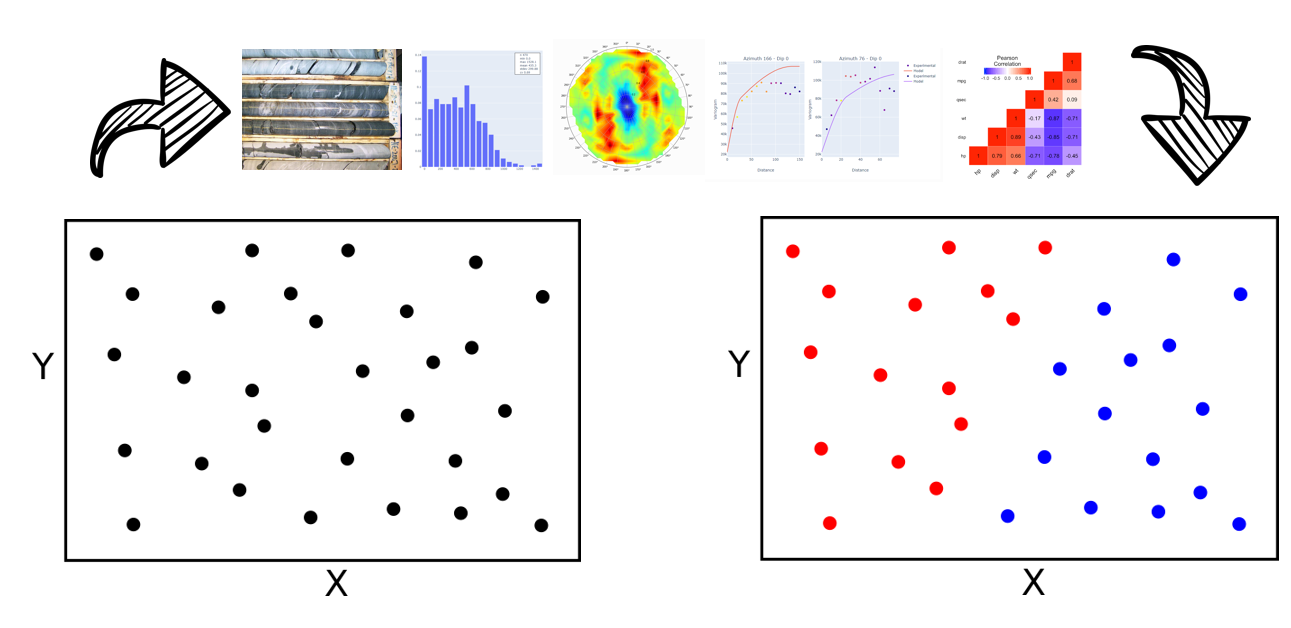
\includegraphics[width=0.8\textwidth]{capitulo_1/imagens/dom_def}
\end{figure}

A definição de diferentes domínios de estimativas, ou zonas estacionárias no interior do depósito, é necessária para a inferência geoestatística. Geralmente, o método usado na construção dos modelos numéricos de teores \cite{mclennanstationarity}. Isto é, os teores em cada domínio estacionário pertencem a populações estatísticas distintas, são caracterizados através de modelos de distribuição e de covariância específicos e devem ser modelados como funções aleatórias estacionárias diferentes. \cite{journel1978mining}. 

Uma função aleatória estacionária é uma representação probabilística de uma propriedade petrofísica com valor esperado e covariância constantes independente da localização \cite{mclennanstationarity}. Estacionariedade, definida por \citeonline{matheron1962traite}, é uma propriedade do modelo de função aleatória, não é uma característica intrínseca da variável. É uma decisão tomada pelo geomodelador e necessária para a inferência. Apesar dos domínios geológicos serem funções aleatórias estacionárias a tomada de decisão na sua determinação não necessariamente deve ser estritamente matemática. Podem ser consideradas propriedades geomecânicas, geometalúrgicas, petroquímicas, a geometria dentre outras. 

Os domínios estacionários não devem ser muito pequenos, dessa forma não incluiriam dados suficientes para descrição e inferência estatística confiável, e nem muito grandes, já que os dados, provavelmente, poderiam ser subdivididos em grupos geologicamente mais homogêneos. A definição adequada dos domínios estacionários é uma etapa importante na avaliação de recursos/reservas, a mistura de populações produz estimativas sub ótimas que superestimam ou subestimam teores e tonelagens. Além disso, nenhuma técnica geoestatística pode compensar uma definição de estacionariedade inadequada \cite{rossi2013mineral}.

Uma vez que os domínios estacionários tenham sido definidos, um modelo tridimensional com os limites de cada função aleatória estacionária deve ser construído: o modelo geológico. É necessário identificar a "jurisdição espacial"\ de cada função aleatória estacionária. A etapa de interpretação e modelagem geológica compreende a definição dos domínios estacionários e a criação do modelo geológico tridimensional que forma o alicerce para todo o trabalho de estimativa subsequente. Muitas vezes, o modelo geológico é o fator de maior importância na estimativas das tonelagens mineralizadas \cite{rossi2013mineral}. A \autoref{ilust_mpod} mostra uma ilustração esquemática do modelo geológico para o exemplo da \autoref{dom_def}.

\begin{figure}[H]
	\centering
	\caption{\label{ilust_mpod}Ilustração esquematizando a modelagem geológica.}
	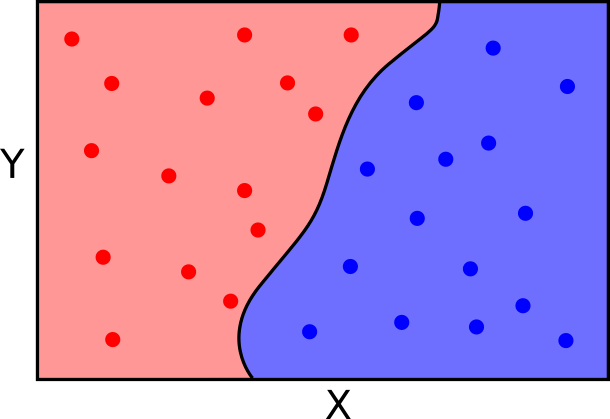
\includegraphics[width=0.6\textwidth]{capitulo_1/imagens/mapa_geomode_det}
\end{figure}

A abordagem tradicional para a criação de modelos geológicos tridimensionais é através da triangulação de polilinhas \footnote{Em computação gráfica: uma linha composta por vários segmentos, usada para compor imagens na tela \cite{oxfordonlinedictionary}.} (\textit{strings}) gerando sólidos que representam os corpos minerais. As polilinhas são digitalizadas manualmente em seções deslocadas, a partir dos dados de sondagem e conhecimento geológico prévio, por um geomodelador. As seções são unidas por linhas guias, que demarcam a conectividade entre as seções digitalizadas para triangulação adequada dos sólidos. Esse procedimento é referido como modelagem geológica explícita, já que os limites entre os diferentes domínios são definidos explicitamente por coordenadas (x,y,z) que posicionam a "colcha de retalhos"\ de triângulos \cite{mclennan2006boundsim,cowan2003practical}. A \autoref{explicitmodeling} ilustra a metodologia explícita para um típico depósito de veio.

\begin{figure}[H]
    \centering
	\caption{\label{explicitmodeling}Ilustração esquematizando a modelagem geológica explícita usando polilinhas e linhas guias.}
	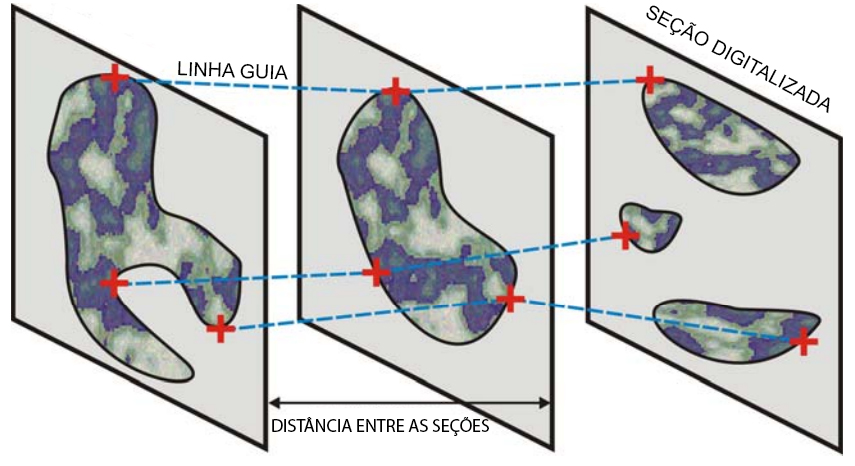
\includegraphics[width=0.8\textwidth]{capitulo_1/imagens/explicitmodeling}
	\legend{Modificado de \citeonline{mclennan2006boundsim}}
\end{figure}

De acordo com \citeonline{mclennan2006boundsim}, embora a metodologia seja direta e simples, principais motivos da sua ampla implementação na prática, e que \textit{softwares} modernos de mineração forneçam ferramentas computacionais para visualizar os dados de sondagem e agilizar o processo de digitalização \cite{silvaenhancedgeomodeling}, existem uma série de limitações e desvantagens. O processo é tedioso e demorado, digitalizar manualmente as polilinhas e uni-las por linhas guia, exige muito tempo de um profissional experiente. Em depósitos de alta complexidade, não é raro o geomodelador trabalhar até três meses no modelo geológico explícito. A geometria dos corpos geológicos muitas vezes precisa ser simplificadas para que o modelo seja concebido em tempo hábil. Por esse motivo, para a maioria das minas, apenas um modelo é construído e mantido, raramente há oportunidade de modelar interpretações geológicas alternativas e comparar estimativas de recursos baseadas em diferentes modelos \cite{cowan2003practical}.

Os modelos criados explicitamente são subjetivos e não replicáveis. O volume mineralizado é essencialmente composto por uma série de pequenas decisões subjetivas, já que cada ponto da polilinha em cada seção é escolhido por um geomodelador. Inevitavelmente, a "assinatura"\ do profissional é impressa nos limites dos domínios geológicos. Geomodeladores diferentes criam modelos diferentes a partir do mesmo banco de dados. Ademais, modelos explícitos são inflexíveis, é laborioso e demorado atualizar modelos explícitos a medida que novos dados são obtidos já que uma nova digitalização manual é necessária.

Embora a metodologia explícita seja demorada, laboriosa, subjetiva, não replicável, inflexível e que avaliar incertezas seja extremamente custoso, o limites entre domínios resultantes, geralmente, são realistas. Realismo geológico é um dos principais objetivos da modelagem e pode ser diretamente controlado durante o processo de digitalização.

\section{Motivação}

Em virtude da onerosidade em construir múltiplos modelos geológicos explícitos, é custoso avaliar a incerteza na localização dos limites dos diferentes domínios entre os dados amostrais, como mostrado na ilustração esquemática na \autoref{incerteza_limites}. Além da tediosa redigitalização manual de polilinhas e retriangulação, não existe forma direta de incorporar múltiplas realizações possíveis para a localização dos limites que representem a incerteza associada.

\begin{figure}[H]
    \centering
	\caption{\label{incerteza_limites}Ilustração esquemática destacando a incerteza na localização do limite entre os domínios azul e vermelho, entre os dados amostrais.}
	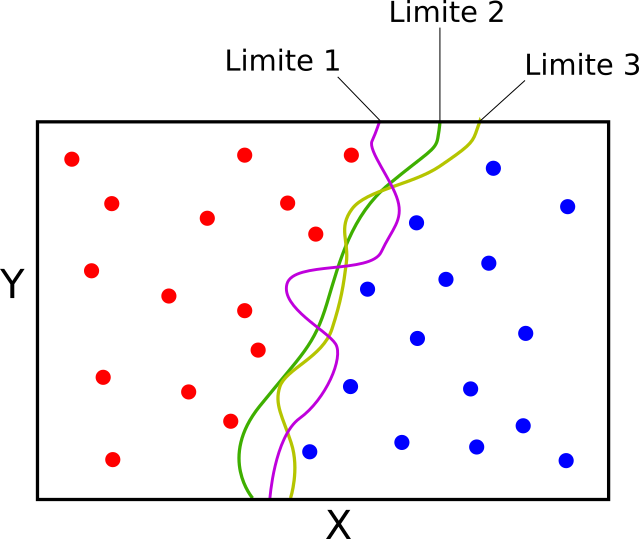
\includegraphics[width=0.6\textwidth]{capitulo_1/imagens/mapa_geomode_stoc}
\end{figure}

Em muitos casos, a incerteza do modelo geológico pode ser uma fonte de incerteza crucial. Em depósitos de veio de ouro, por exemplo, o volume mineralizado é um indicador econômico vital para o gerenciamento do projeto. Ignorar a incerteza volumétrica, considerando apenas um único modelo geológico explícito, pode ser ser devastador para o empreendimento. A incerteza associada ao modelo geológico deve ser avaliada.

Dadas as desvantagens do método explícito de modelagem geológica, pesquisas vêm sendo realizadas com o objetivo de automatizar, ou pelo menos, semi automatizar a modelagem e avaliar incerteza dos modelos geológicos.

Alguns dos métodos de simulação para variáveis categóricas, amplamente utilizados pela indústria da mineração, geram realizações que apresentam excessivo ruído. Além da necessidade de avaliar a incerteza dos modelos geológicos, existe também a preocupação de que os modelos finais apresentem limites contínuos e realistas entre as diferentes litologias do depósito. Não só para que os modelos tenham uma aparência mais agradável aos olhos, mas também para que a tarefa de definir \textit{diglines}, entre minério e estéril, seja facilitada e menos subjetiva.

\section{Declaração de tese}

\begin{tcolorbox}
A modelagem geológica implícita com funções distância assinaladas vem sendo utilizada há mais de uma década com sucesso como uma alternativa matemática à modelagem explícita na criação de modelos geológicos determinísticos. A metodologia está presente em diversos softwares comerciais de ampla utilização na indústria. Embora exista a necessidade de avaliar a incerteza associada ao modelo geológico, não há na literatura diferentes opções de métodos de avaliação de incerteza baseadas em funções distância assinaladas, especialmente para modelos multi-categóricos.
\end{tcolorbox}

\section{Objetivos}

O objetivo dessa tese é propor e investigar três diferentes metodologias para avaliação de incerteza em modelos geológicos   multi-categóricos usando funções distância assinaladas. As realizações obtidas a partir das metodologias propostas devem apresentar feições geológicas realistas e contínuas. Os métodos foram desenvolvidos e implementados em forma de \textit{plug-ins} para o \textit{software SGeMS/AR2GeMS} \cite{remy2009applied} ou \textit{jupyter notebooks} baseados em \textit{softwares} da biblioteca \textit{GSLib} \cite{deutsch1992geostatistical}.

\subsection{Desenvolvimento de software}

Foi desenvolvida uma \textit{suite} de \textit{plug-ins} de modelagem geológica para o \textit{software} geoestatístico \textit{SGeMS/AR2GeMS}: \href{https://github.com/robertorolo/LPM-Geomod_Suite}{LPM-Geomod-Suite}. Os \textit{plug-ins} abrangem todas as etapas da modelagem geológica com funções distância assinaladas e indicadores desde transformações, interpolação, e avaliação da incerteza associada ao modelo geológico. 

Um manual de instalação e uso dos \textit{plug-ins} é apresentado no \autoref{software}. 

\subsection{Avaliação de incerteza pela parametrização do suporte do \textit{kernel}}

É proposto um método para avaliação de incerteza baseado na parametrização do suporte do \textit{kernel}, que é a base para a interpolação das distâncias assinaladas utilizando funções de bases radiais (RBF). O \textit{kernel} é análogo ao variograma da krigagem. Para cada uma das variáveis, são geradas interpolações: para um cenário base, sem parametrização, um cenário otimista e um cenário pessimista. As diferentes propriedades interpoladas são combinadas para gerar diferentes realizações para o modelo geológico.  

\subsection{Avaliação de incerteza usando funções distância assinaladas e campos de probabilidade}

É proposto um método de avaliação de incerteza utilizando funções distância assinaladas e campos de probabilidade. Uma zona de incerteza é definida ao redor dos contatos, então, as distâncias assinaladas interpoladas no interior da zona de incerteza são transformadas em probabilidades. Em seguida, os campos de probabilidades gerados a partir de simulações Gaussianas não condicionais são utilizados para simular as diferentes realizações para o modelo geológico a partir do método de Monte Carlo.

\subsection{Simulação de contatos hierárquica para múltiplas categorias}

Uma adaptação do método proposto por \citeonline{wilde2012kriging} para múltiplas categorias simultâneas é proposto. Um algoritmo que identifica e define a frequência de ocorrência dos diferentes contatos é usado para agrupá-los de forma hierárquica. Os contatos representados por cada grupo são simulados de forma independente e a regra hierárquica é usada para construir as diferentes realizações do modelo geológico multi-categórico. 

\section{Estrutura da tese}

O capítulo 1 dessa tese traz uma introdução ao assunto modelagem geológica e avaliação de incerteza e apresenta: a motivação, declaração e objetivos da tese.

O capítulo 2 é uma revisão extensiva da literatura em modelagem geológica e avaliação de incerteza em modelos geológicos usando funções distância assinaladas. 

O capítulo 3 apresenta as metodologias propostas utilizando o conhecido \textit{dataset} \textit{Swiss Jura} \cite{goovaerts1997geostatistics} como prova de conceito em 2D. Um estudo de caso é conduzido para cada uma das metodologias propostas mostrando sua eficiência. As características e particularidades de cada uma delas e os resultados obtidos são discutidos.

Finalmente, o capítulo 4 apresenta as observações finais, um sumário das contribuições da tese e sugere trabalhos futuros.
\chapter{Revisão bibliográfica}

Esse capítulo é uma revisão da literatura em modelagem geológica automática e avaliação de incerteza em modelos geológicos com ênfase no uso de funções distância assinaladas.

\section{Modelagem geológica determinística}

A dispendiosidade na construção e a inflexibilidade dos modelos explícitos impulsionaram o desenvolvimento de técnicas de modelagem geológica automáticas. As técnicas determinísticas geram apenas um único modelo, consequentemente, não possibilitando a avaliação da incerteza associada ao modelo geológico.

\subsection{Vizinho mais próximo}

Métodos geométricos menos sofisticados, como o vizinho mais próximo podem ser utilizados na criação automática de modelos geológicos determinísticos. Esse algoritmo constrói ao redor de cada amostra sua área de influência, ou volume de influência em três dimensões. A toda a área de influência é atribuída a categoria, ou litologia, correspondente àquela amostra.

\subsection{Aprendizado de máquina}

Métodos baseados em aprendizado de máquina também podem ser utilizados. \citeonline{smirnoff2008support} propuseram o uso de máquina de vetores de suporte (\textit{support vector machine}) para a criação de modelos geológicos determinísticos multi-categóricos a partir de amostras esparsas de diferentes origens.

\subsection{Krigagem dos indicadores}\label{ik}

Considere $\{S(\alpha), \alpha=1,...,n\}$ o conjunto de observações do atributo categórico s medidos em cada local $\alpha$. O conjunto dos K possíveis estados $s_{k}$ que cada valor $S(\alpha)$ pode assumir é denotado por $\{s_{1}, ..., s_{k}\}$. Por exemplo, $s(\alpha)=s_{k}$ se o estado $s_{k}$ foi observado no enésimo local $\alpha$.

Os estados K são exaustivos e mutualmente excludentes, já que cada indivíduo pertence a um e apenas um estado $s_{k}$. O histograma de dados categóricos é completamente descrito por uma tabela de frequência , que lista os K estados se sua frequência de ocorrência. A frequência de ocorrência do estado $s_{k}$, denotada por $f(s_{k})$, pode ser expressa como uma média aritmética dos n indicadores de acordo com a \autoref{ik1} \cite{goovaerts1997geostatistics}:

\begin{equation}
	f(s_{k})=\frac{1}{n}\sum_{\alpha=1}^{n}i(\alpha;s_{k})
	\label{ik1}
\end{equation}

Onde os indicadores $i(\alpha;s_{k})$ associados com cada enésimo indivíduos pode assumir o valor se o estado $s_{k}$ for observado, e 0 caso contrário.

Considere o problema em modelar a incerteza acerca do estado $s_{k}$ do atributo categ;orico s no local não amostrado u. Para o nível de informação (n) essa incerteza é modelada a partir da função de distribuição de probabilidade condicional (ccdf) da variável discreta s(u) de acordo com a \autoref{ik2}:

\begin{equation}
	(p(u;s_{k})|(n))=Prob(S(u)=s_{k}|(n)), k=1,...,n
	\label{ik2}
\end{equation}

Onde a informação condicionante consiste nos n dados categóricos $s(u_{\alpha})$ vizinhos.

Cada probabilidade condicional $p(u;s_{k})$ é também o valor esperado condicional do indicador da classe, dada a informação (n). Como mostrado na \autoref{ik3}:

\begin{equation}
	(p(u;s_{k})|(n))=E(I(u;s_{k})|(n))
	\label{ik3}
\end{equation}

Com $I(u;s_{k})=1$ se $S(u)=s_{k}$ e 0 caso contrário. Então o ccdf da variável categórica $S(u)$ pode ser modelado a partir da krigagem dos indicadores que é um estimador da média (valor esperado).

O algoritmo apresentado pode ser usado para estimar cada probabilidade condicional $(p(u;s_{k})|(n))$ como uma combinação linear dos indicadores $I(u;s_{k})$ na vizinhança de busca.

Em cada local estimado u a probabilidade deve estar entre  [0,1] e seu somatório deve ser 1. Em alguns casos os pesos de krigagem podem acarretar estimativas que não obedecem esses requisitos. Nesses casos deve ser feita a correção de relação de ordem. A categoria escolhida para cada nó, é aquela com maior probabilidade de ocorrência.

\subsection{Métodos implícitos}

A família de métodos ditos métodos implícitos compreendem técnicas importadas da computação gráfica. O uso da modelagem implícita foi introduzida no campo da computação gráfica para a geração de objetos de diferentes geometrias e complexidades por  \citeonline{bloomenthal1997introduction}. A ideia geral é usar uma função implícita para demarcar regiões de diferentes formas e extensões no espaço. \citeonline{cowan2002rapid} e \citeonline{cowan2003practical} popularizaram a modelagem implícita no contexto geológico, baseados no trabalho de \citeonline{savchenko}, que modela objetos tridimensionais a partir de dados esparsos interpolando uma função volume.

Modelos geológicos implícitos são criados a partir de dados esparsos, geralmente, dados categóricos (\autoref{imp_mod} (a)). Os pontos amostrais podem ser usados para derivar uma função implícita que fornece uma representação matemática contínua de um atributo através de um volume, um campo escalar ou modelo implícito (\autoref{imp_mod} (b)). Modelos implícitos contém um número infinito de isosuperfícies. Para visualizar o modelo geológico uma isosuperfície específica deve ser extraída do modelo e mostrada no espaço tridimensional (geralmente a isosuperfície zero), $f(x,y,z)=s$, onde $s$ é o valor de interesse no campo escalar (\autoref{imp_mod} (c)). A localização dessa superfície é conhecida implicitamente como função da localização no domínio \cite{martin2017implicitmodeling}.

\begin{figure}[H]
    \centering
	\caption{\label{imp_mod}Ilustração esquemática da modelagem geológica implícita.}
	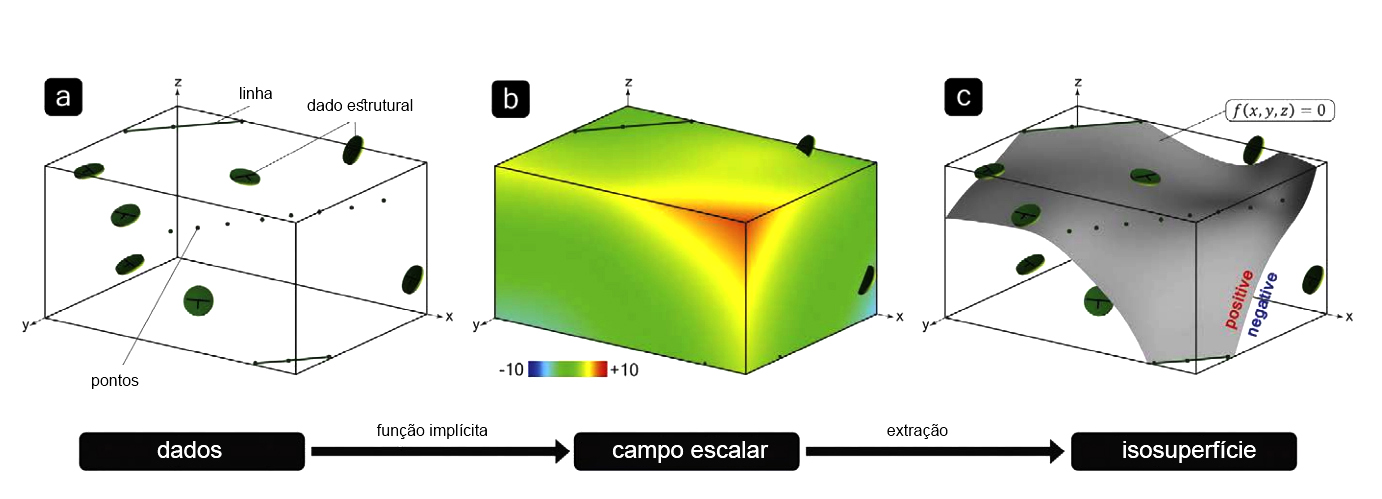
\includegraphics[width=\textwidth]{capitulo_2/imagens/implicit_modelig_pt_1.jpg}
	\legend{Modificado de \cite{aillerespresentation}}
\end{figure}

Diferentes tipos de dados amostrais podem ser usados para derivar diferentes funções volume na modelagem implícita. \citeonline{mallet2004space} propõe uma função volumétrica cronológica, levando em consideração a posição estratigráfica das diferentes unidades geológicas, enquanto \citeonline{lajaunie1997foliation, chiles2004modelling, calcagno2008geological} usam co-krigagem de incrementos em um campo potencial, omitindo a função volume. O procedimento não é simples já que a covariância do campo potencial é particularmente difícil de inferir uma vez que não há \textit{hard data} de campo potencial disponível.

A função volume mais comumente utilizada é a função distância assinalada \cite{osherlevelsetmethods}. A aplicação dessa metodologia é encontrada por toda a literatura de interpolação de dados esparsos, uma das aplicações é a reconstrução de superfícies a partir de escaneamento. Na modelagem geológica, a metodologia é competente em capturar a geometria e extensão de corpos geológicos e tem sido aplicada com sucesso há mais de uma década na exploração mineral tendo ganhado espaço em diferentes \textit{softwares} comerciais. Para bancos de dados pontuais, que representam a posição  de diferentes litologias no espaço, o uso das funções distância assinaladas torna os processos de interpretação, cálculo, modelagem, modificação do modelo de acordo com a interpretação dos geomodeladores e avaliação da incerteza diretos e rápidos. Além disso, informações a respeito da orientação das unidades geológicas (dados estruturais) podem ser imputada como restrição na criação do modelo geológico \cite{martin2017implicitmodeling}.

As próximas seções trazem uma revisão bibliográfica extensiva da modelagem geológica com funções distância assinaladas.

\subsection{Modelagem geológica com funções distância assinaladas}

Para  ilustrar a metodologia será utilizado o \textit{dataset} \textit{Swiss Jura} \cite{goovaerts1997geostatistics}. O \textit{dataset} compreende 259 amostras da propriedade \textit{rock type} (RT). Um mapa com a localização das amostras é mostrado na \autoref{jura_pontos}.

A variável RT possui cinco categorias: \textit{Argovian; Kimmeridgian; Sequian;
Portlandian; e Quartenary}. A área é coberta parcialmente com amostras uniformemente espaçadas, algumas áreas são densamente amostradas com agrupamento adicional de amostras.

\begin{figure}[H]
	\centering
	\caption{\label{jura_pontos}Mapa de localização das 259 amostras do \textit{dataset} \textit{Swiss Jura}.}
	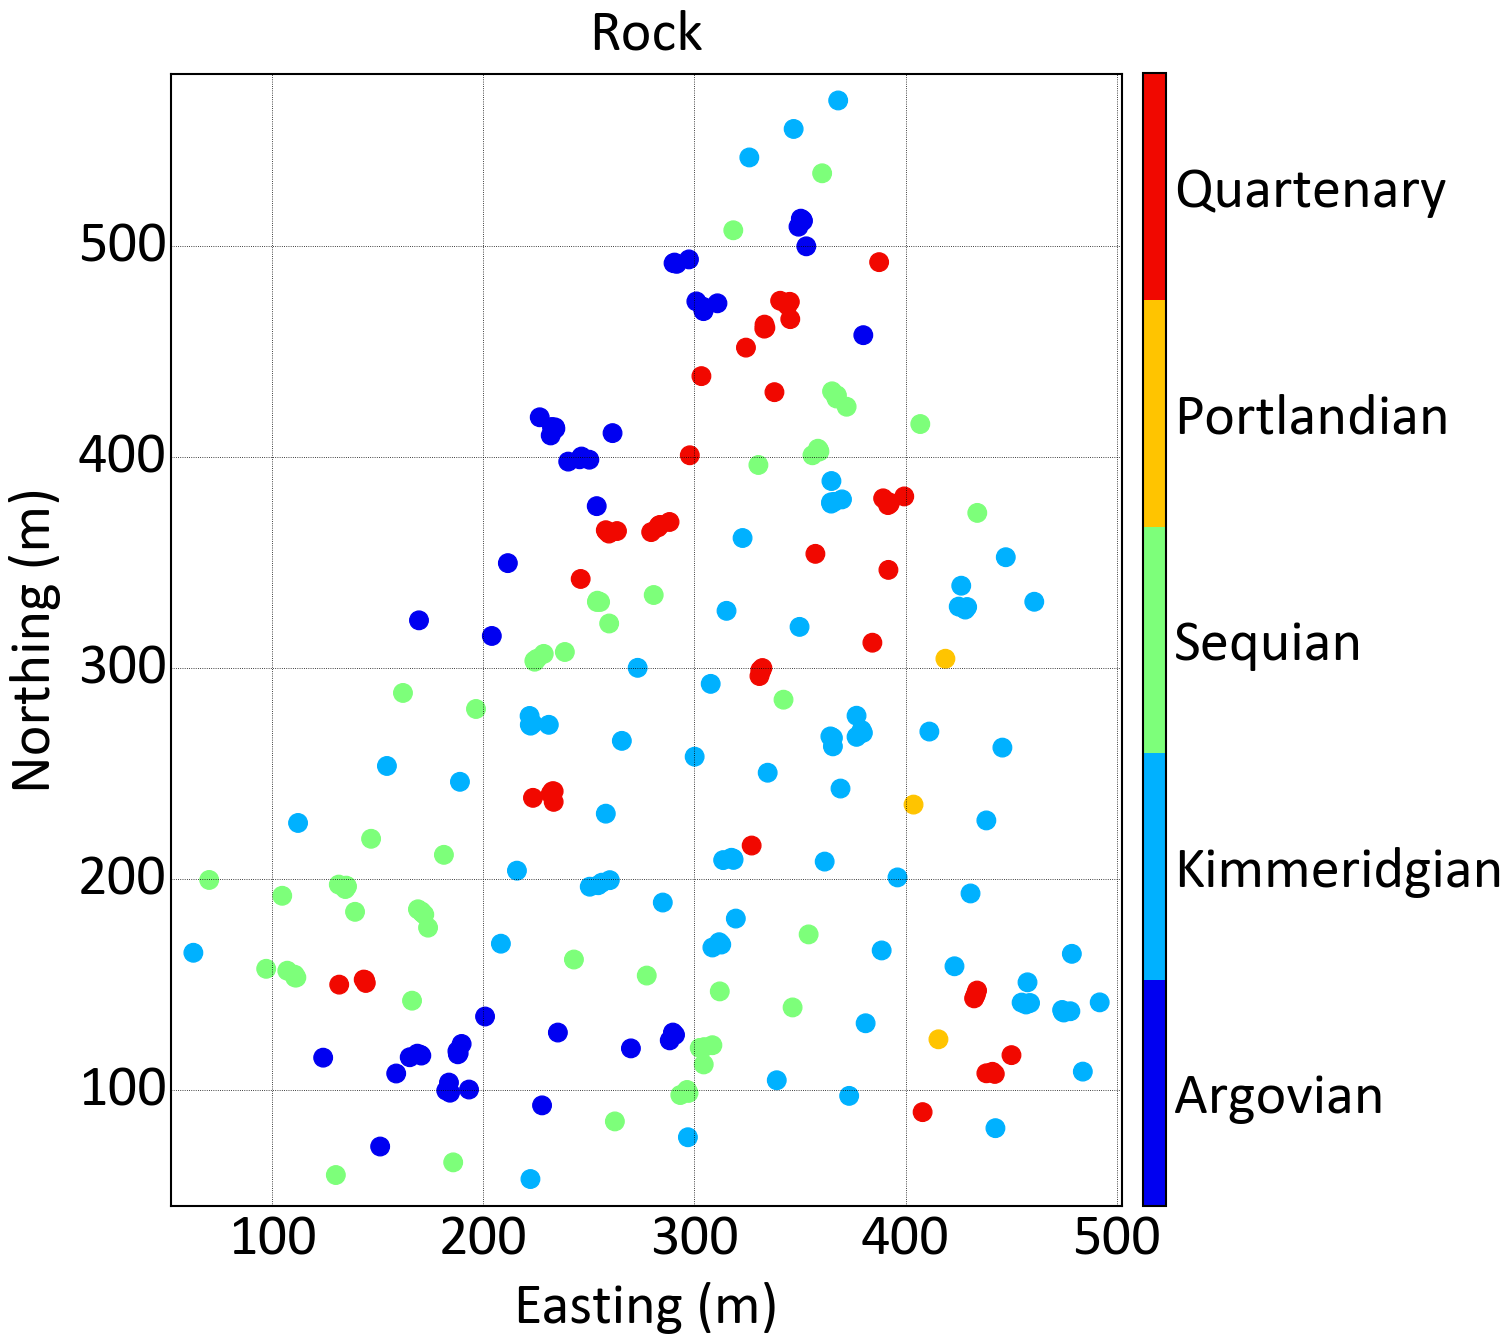
\includegraphics[width=0.6\textwidth]{capitulo_2/imagens/points.png}
\end{figure}

\subsubsection{Cálculo das distâncias assinaladas}\label{calc_dist}

O primeiro passo no cálculo das distâncias assinaladas é transformar as amostras ${z(u_\alpha),\alpha=1,...,n}$ em indicadores binários de acordo com a \autoref{eq_ind}, especificando se a amostra pertence ou não ao domínio $k$ que está sendo modelado.

\begin{equation}
	i_k(u_\alpha)=\begin{cases}
	1,\:\textrm{se}\:z(u_\alpha)\:\textrm{se pertence ao domínio $k$}\\
	0,\:\textrm{se}\:z(u_\alpha)\:\textrm{caso contrário}\end{cases}
    \label{eq_ind}
\end{equation}

Como exemplo será utilizada a categoria Quaternary do \textit{Swiss Jura}. A \autoref{ind_5} mostra as amostras do \textit{Swiss Jura} transformadas em indicadores para essa categoria.

\begin{figure}[H]
	\centering
	\caption{\label{ind_5}Mapa de localização das 259 amostras dos indicadores para a categoria Quaternary do \textit{dataset} \textit{Swiss Jura}.}
	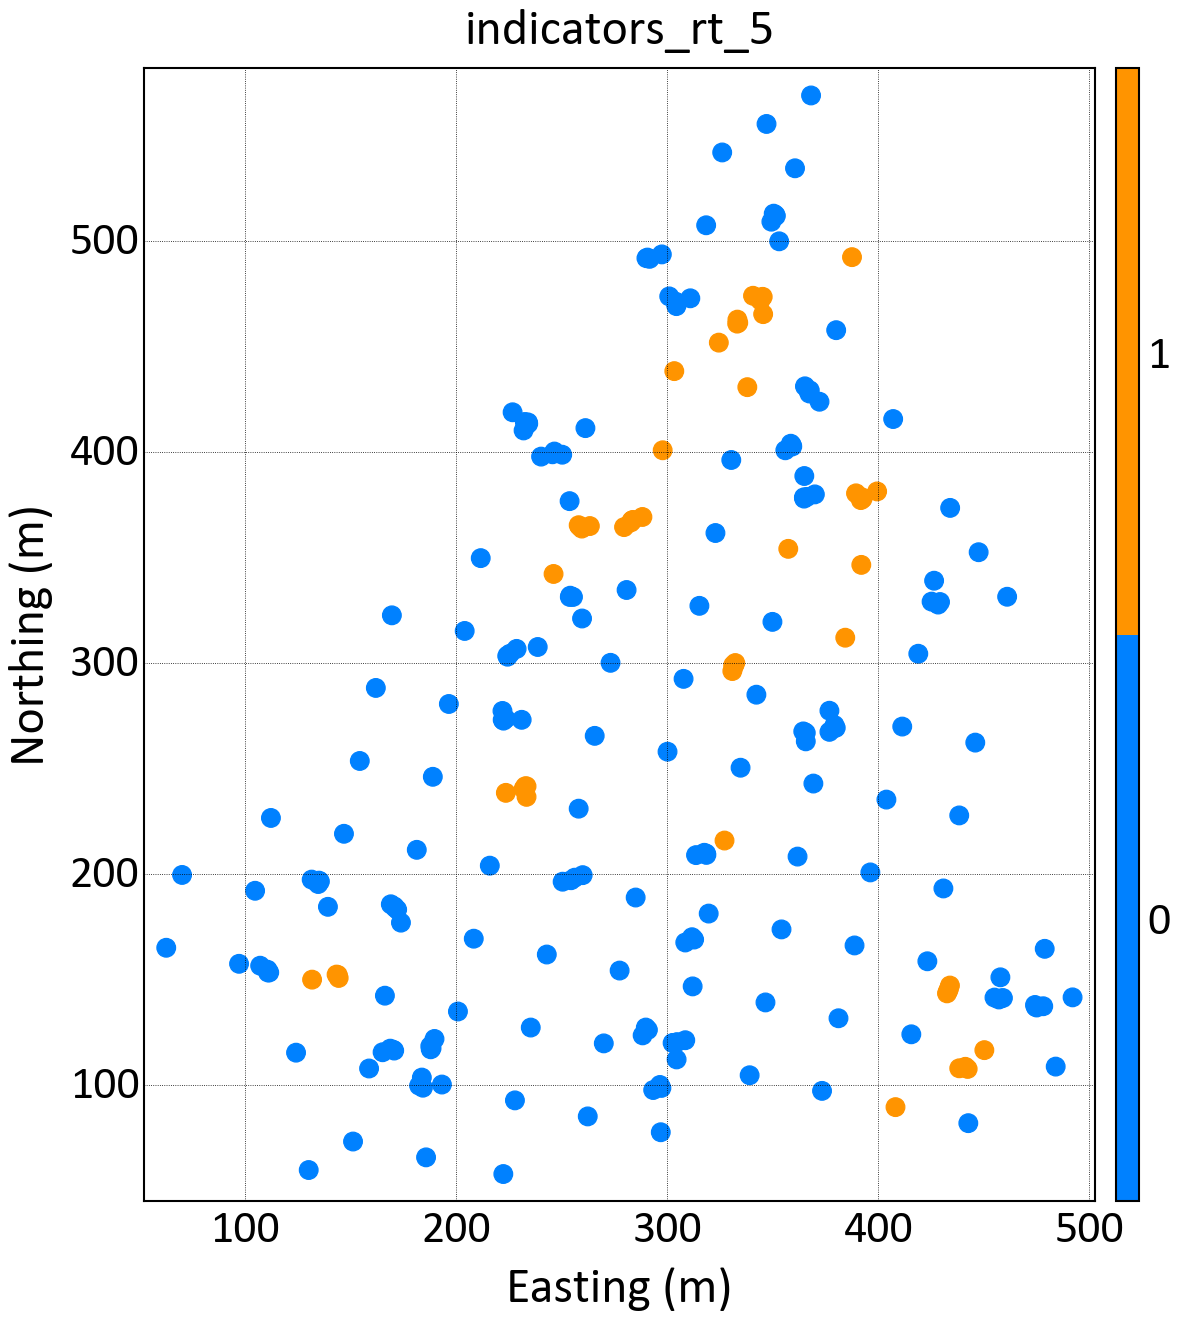
\includegraphics[width=0.6\textwidth]{capitulo_2/imagens/ind5.png}
\end{figure}

O segundo passo é o cálculo das distâncias assinaladas. Para cada ponto amostral, a menor distância euclideana até um outro ponto amostral que pertença a um indicador oposto é computada, e esse valor atribuído àquele ponto, com o sinal negativo caso pertença ao domínio modelado e com o sinal positivo, caso contrário, como ilustrado na \autoref{2d_ex}.

\begin{figure}[H]
    \centering
	\caption{\label{2d_ex}Ilustração esquemática mostrando o cálculo das distâncias assinaladas.}
	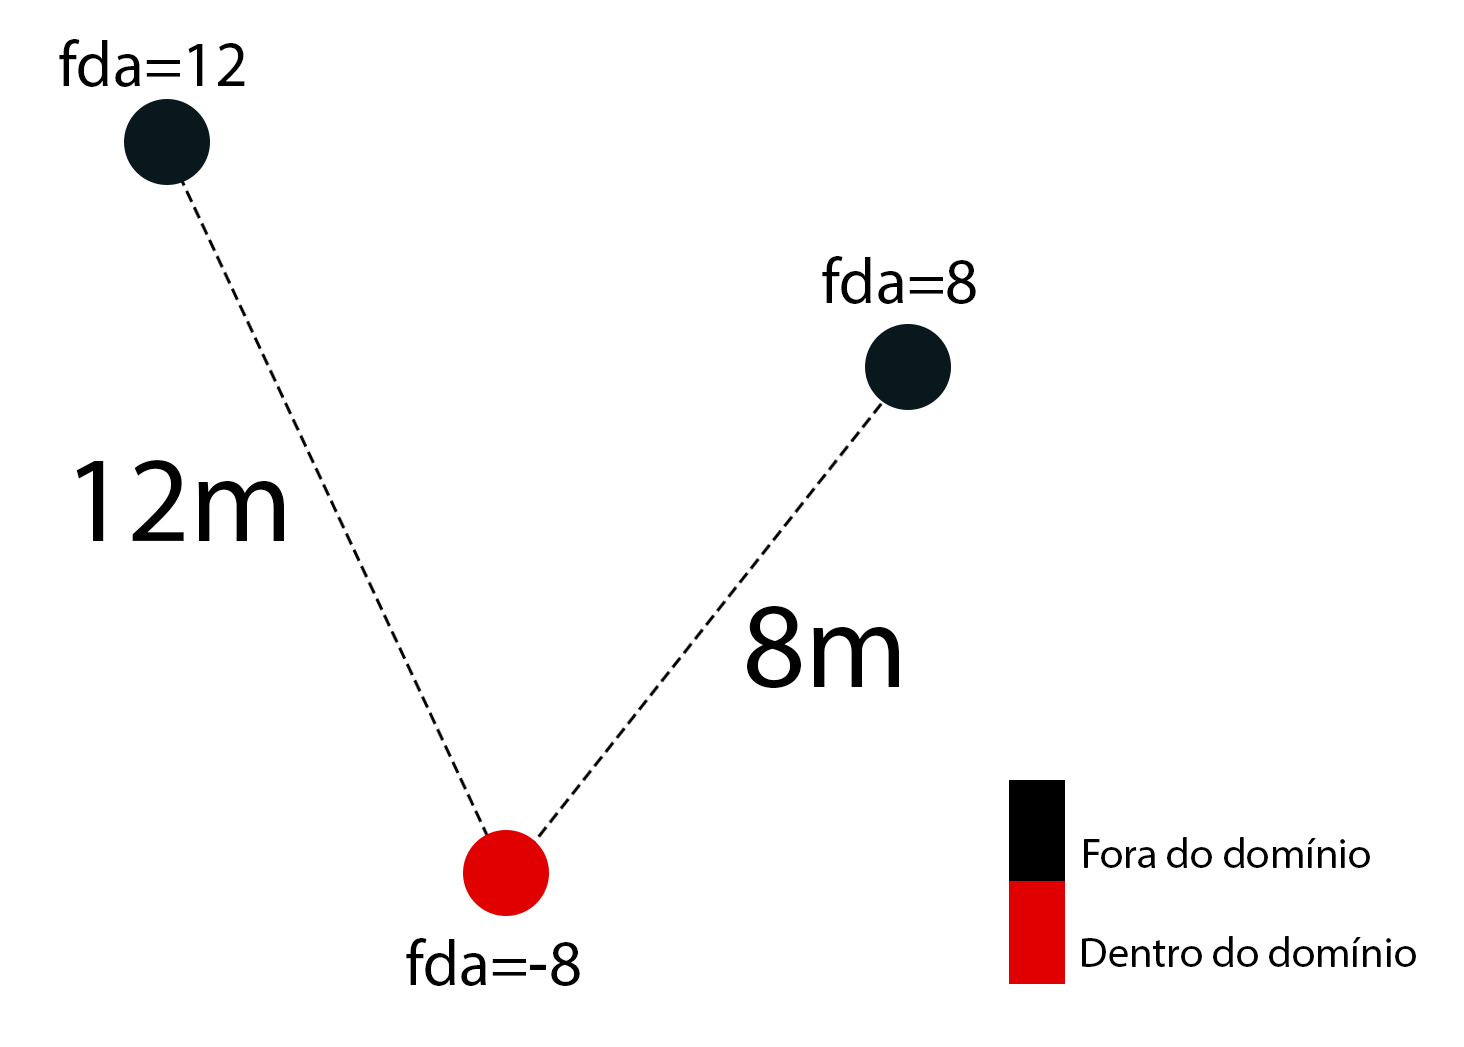
\includegraphics[width=0.6\textwidth]{capitulo_2/imagens/2d_ex.jpg}
\end{figure}

Desse modo, o valor da função distância assinalada $d_k$ para a o domínio $k$ modelado no local $u_\alpha$ é:

\begin{equation}
	d_{k}(u_{\alpha})=\begin{cases}
	-\parallel u_\alpha-u_\beta\parallel,\:\textrm{se $u_\alpha$ pertence ao domínio}\\
	+\parallel u_\alpha-u_\beta\parallel,\:\textrm{se $u_\alpha$ não pertence ao domínio}\end{cases}
    \label{eq_mult_sg}
\end{equation}

O local $u_\beta$ corresponde à amostra mais próxima codificada com um indicador diferente de $u_\alpha$.

A \autoref{sd5} mostra as distâncias assinaladas calculadas para a categoria Quaternary do \textit{Swiss Jura}.

\begin{figure}[H]
	\centering
	\caption{\label{sd5}Mapa de localização das distâncias assinaladas para a categoria Quaternary do \textit{dataset} \textit{Swiss Jura}.}
	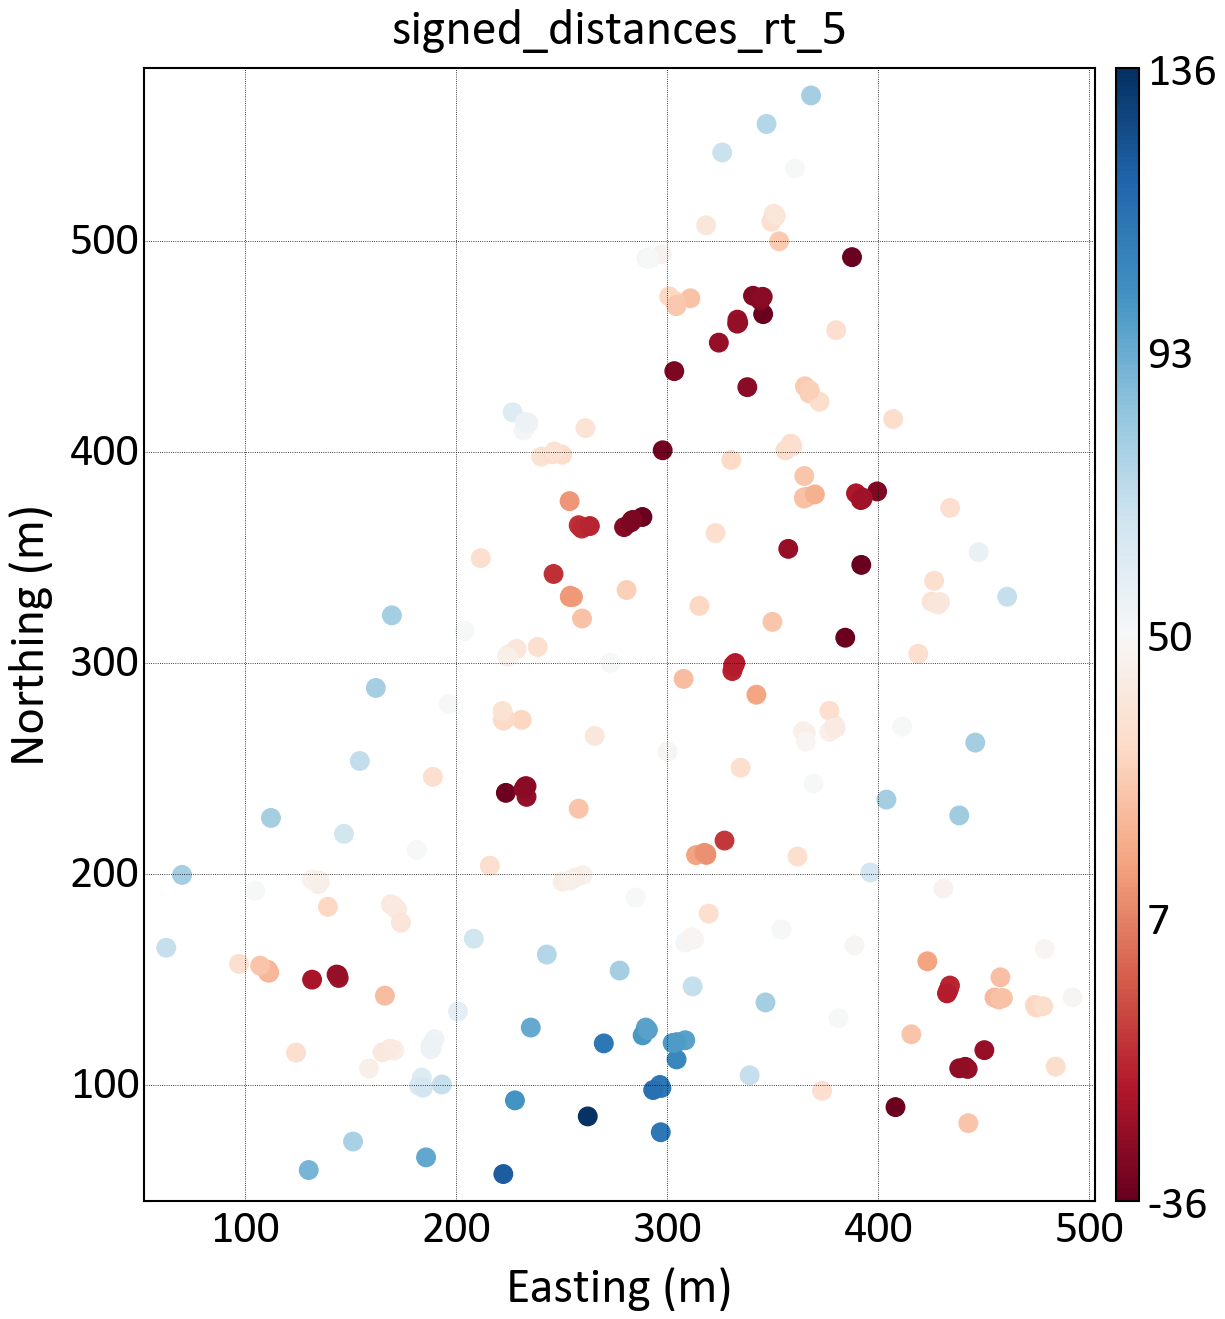
\includegraphics[width=0.6\textwidth]{capitulo_2/imagens/sd5.png}
\end{figure}

Para corpos geológicos que se estendem muito mais em uma direção em relação às demais, como os corpos tabulares por exemplo, as distâncias calculadas podem ser anisotrópicas. Sendo assim, as coordenadas originais $x$, $y$ e $z$ dos dados devem ser rotacionadas e/ou contraídas/dilatadas, a partir da transformação da \autoref{eq_rot_matrix}. Então, as distâncias euclideanas (\autoref{eq_mult_sg}) são calculadas normalmente para as novas coordenadas $x''$, $y''$, $z''$.

\begin{equation}
\resizebox{.9 \textwidth}{!}{%
$
\begin{bmatrix} x'' \\ y'' \\ z'' \end{bmatrix} = \begin{bmatrix} \frac{1}{a_{max}} & 0 & 0 \\ 0 & \frac{1}{a_{min}} & 0 \\ 0 & 0 & \frac{1}{a_{vert}} \end{bmatrix} \\ \begin{bmatrix}\cos\alpha\cos\phi-\sin\alpha\sin\beta\sin\phi & -\sin\alpha\cos\phi-\cos\alpha\sin\beta\sin\phi & \cos\beta\sin\phi \\ \sin\alpha\cos\beta & \cos\alpha\cos\beta & \sin\beta \\ -\cos\alpha\sin\phi-\sin\alpha\sin\beta\cos\phi & \sin\alpha\sin\phi-\cos\alpha\sin\beta\cos\phi & \cos\beta\cos\phi \end{bmatrix} \begin{bmatrix} x \\ y \\ z \end{bmatrix}
$
}
\label{eq_rot_matrix}
\end{equation}

Onde $a_{max}$, $a_{min}$ e $a_{vert}$ são as dimensões dos eixos máximo, médio e mínimo, e $\alpha$, $\beta$ e $\phi$, os ângulos de azimute, mergulho e \textit{rake} que caracterizam os eixos de anisotropia.

\subsubsection{Variografia}

No caso das distâncias assinaladas, obter um modelo de covariância a partir dos variogramas experimentais não é trivial. Distâncias assinaladas não são estacionárias, por isso, o variograma não se estabiliza em um patamar. Além disso, o caráter extremamente contínuo das distâncias torna a identificação analítica das direções principais um processo embaraçoso.

\citeonline{manchuck_deutsch_Geometric} sugerem alternativas para modelagem do variograma das distâncias:

\begin{itemize}
    \item Treinar o variograma usando validação cruzada;
    \item Tentar modelar interativamente os variogramas experimentais;
    \item Calcular e modelar os variogramas para as propriedades de indicadores e transformá-los em um equivalente Gaussiano para as distâncias assinaladas baseado na similidade entre a simulação Gaussiana truncada e a modelagem geológica com funções distância assinaladas. Um campo Gaussiano diferenciável e contínuo é gerado e truncado em um limiar para que a proporção correta de um indicador particular seja o resultado. Entretanto, na prática, o variograma dos indicadores é usado para parametrizar o variograma das distâncias assinaladas de forma direta \cite{martin2017implicitmodeling};
    \item Inferir um modelo de covariância plausível a partir de mapas delineados a mão em \textit{softwares} de iso-contorno.
\end{itemize}

Uma outra alternativa ao cálculo e modelagem de variogramas é o uso de tabelas de covariância proposto por \citeonline{kloechner_cov_table}, esse estudo propõe a substituição da modelagem tradicional dos variogramas por tabelas de covariância, tornando o processo de modelagem geológica completamente automático e livre da subjetividade do geomodelador.

O alcance do variograma, juntamente com a anisotropia, controlam a extensão e forma dos domínios modelados. Os variogramas experimentais das distâncias assinaladas não exibem efeito pepita. Porém, pode ser adicionado arbitrariamente pelo usuário para controlar a interconectividade dos domínios, adicionar ruído ao modelo quando desejável e controlar a extrapolação que pode ser ser excessiva em alguns casos devido à alta continuidade dos modelos Gaussianos.

A \autoref{jura_vargs} mostra o variograma omnidirecional dos indicadores para as categorias do \textit{Swiss Jura}. Os variogramas foram modelados com uma estrutura esférica e efeito pepita zero.

\begin{figure}[H]
    \caption{Variogramas omnidirecionais dos indicadores.} \label{jura_vargs}
     \centering
     \subfloat[][Argovian.]{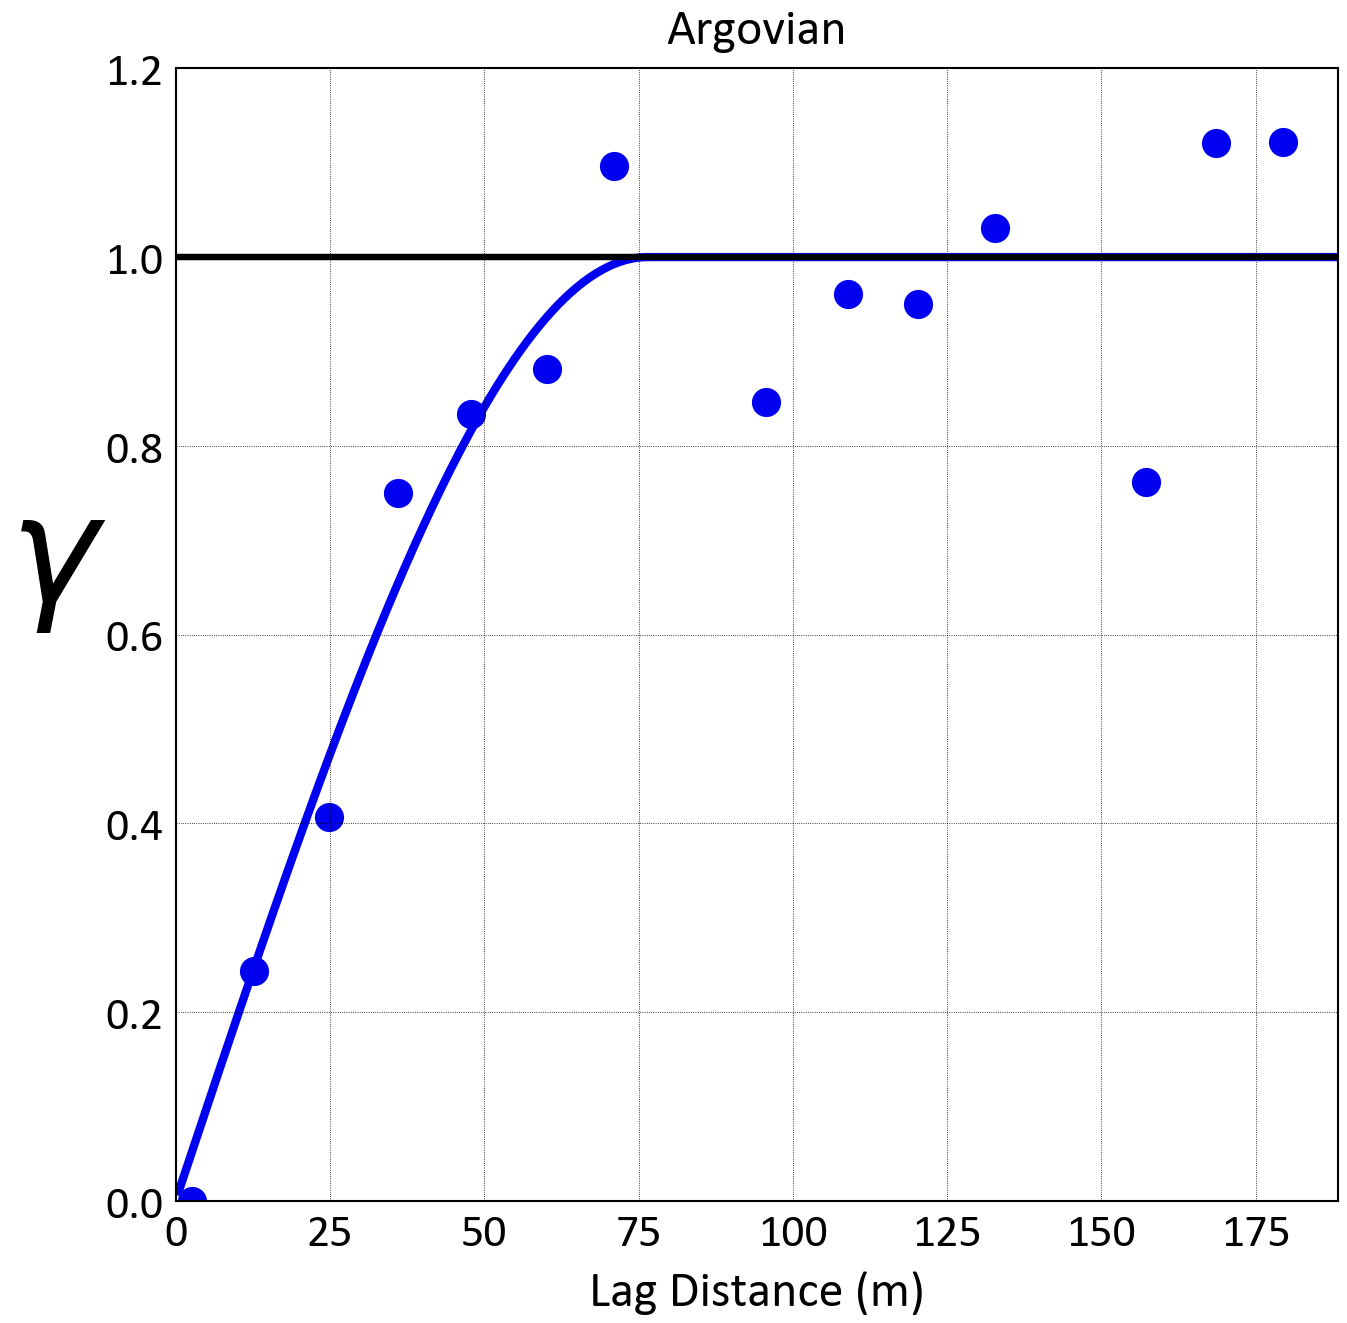
\includegraphics[width=0.45\textwidth]{capitulo_2/imagens/jura_var_1.png}\label{fig:jv1}}
     \hspace{1em}
     \subfloat[][Kimmeridgian.]{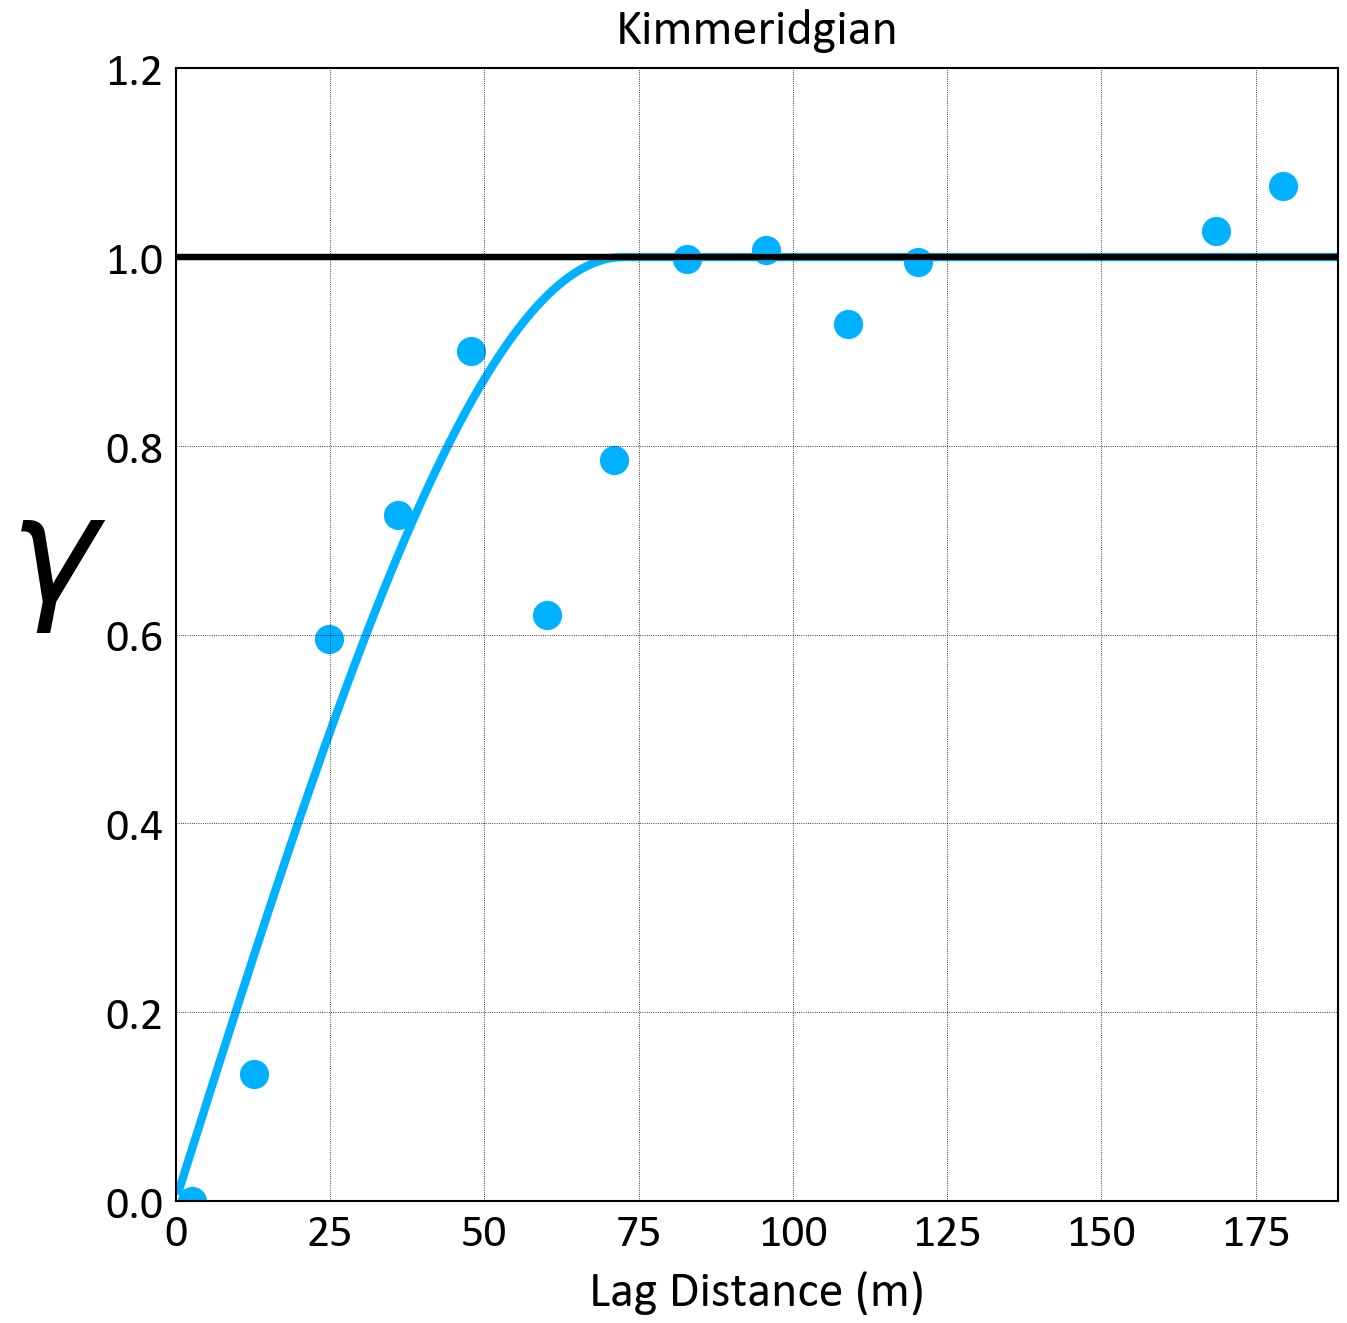
\includegraphics[width=0.45\textwidth]{capitulo_2/imagens/jura_var_2.png}\label{fig:jv2}}\\
    \subfloat[][Sequian.]{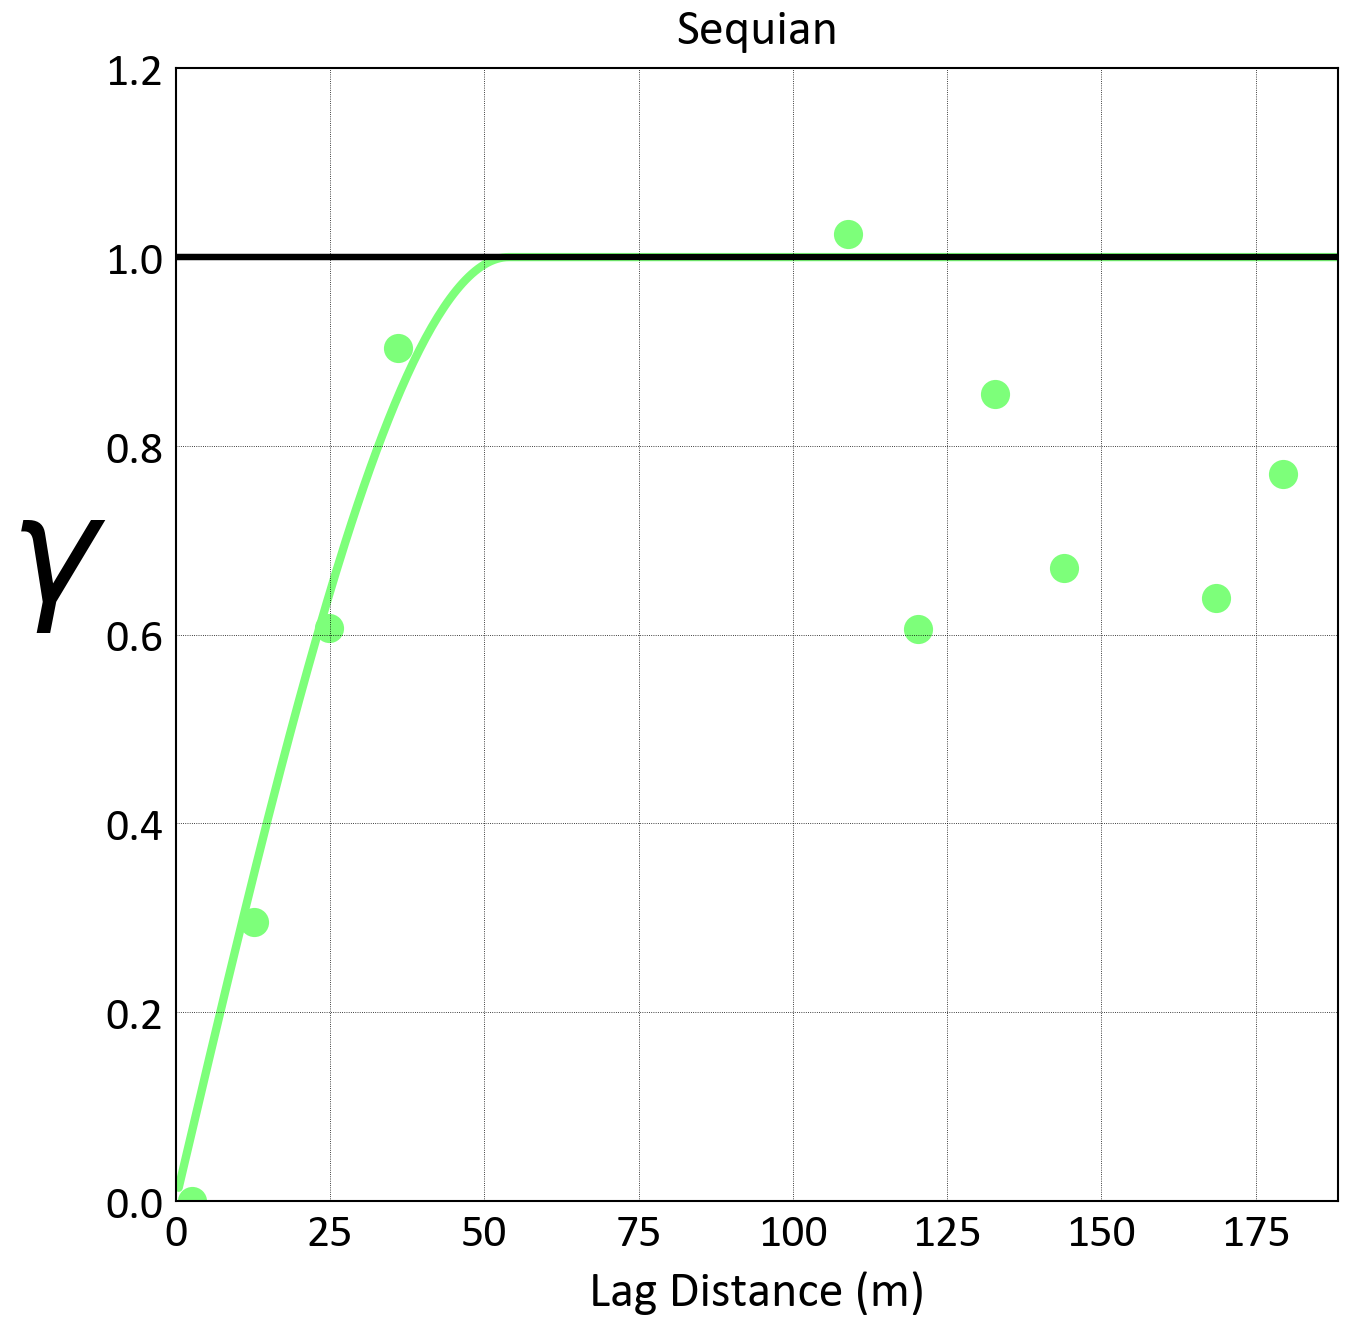
\includegraphics[width=0.45\textwidth]{capitulo_2/imagens/jura_var_3.png}\label{fig:jv3}}
    \hspace{1em}
    \subfloat[][Portland.]{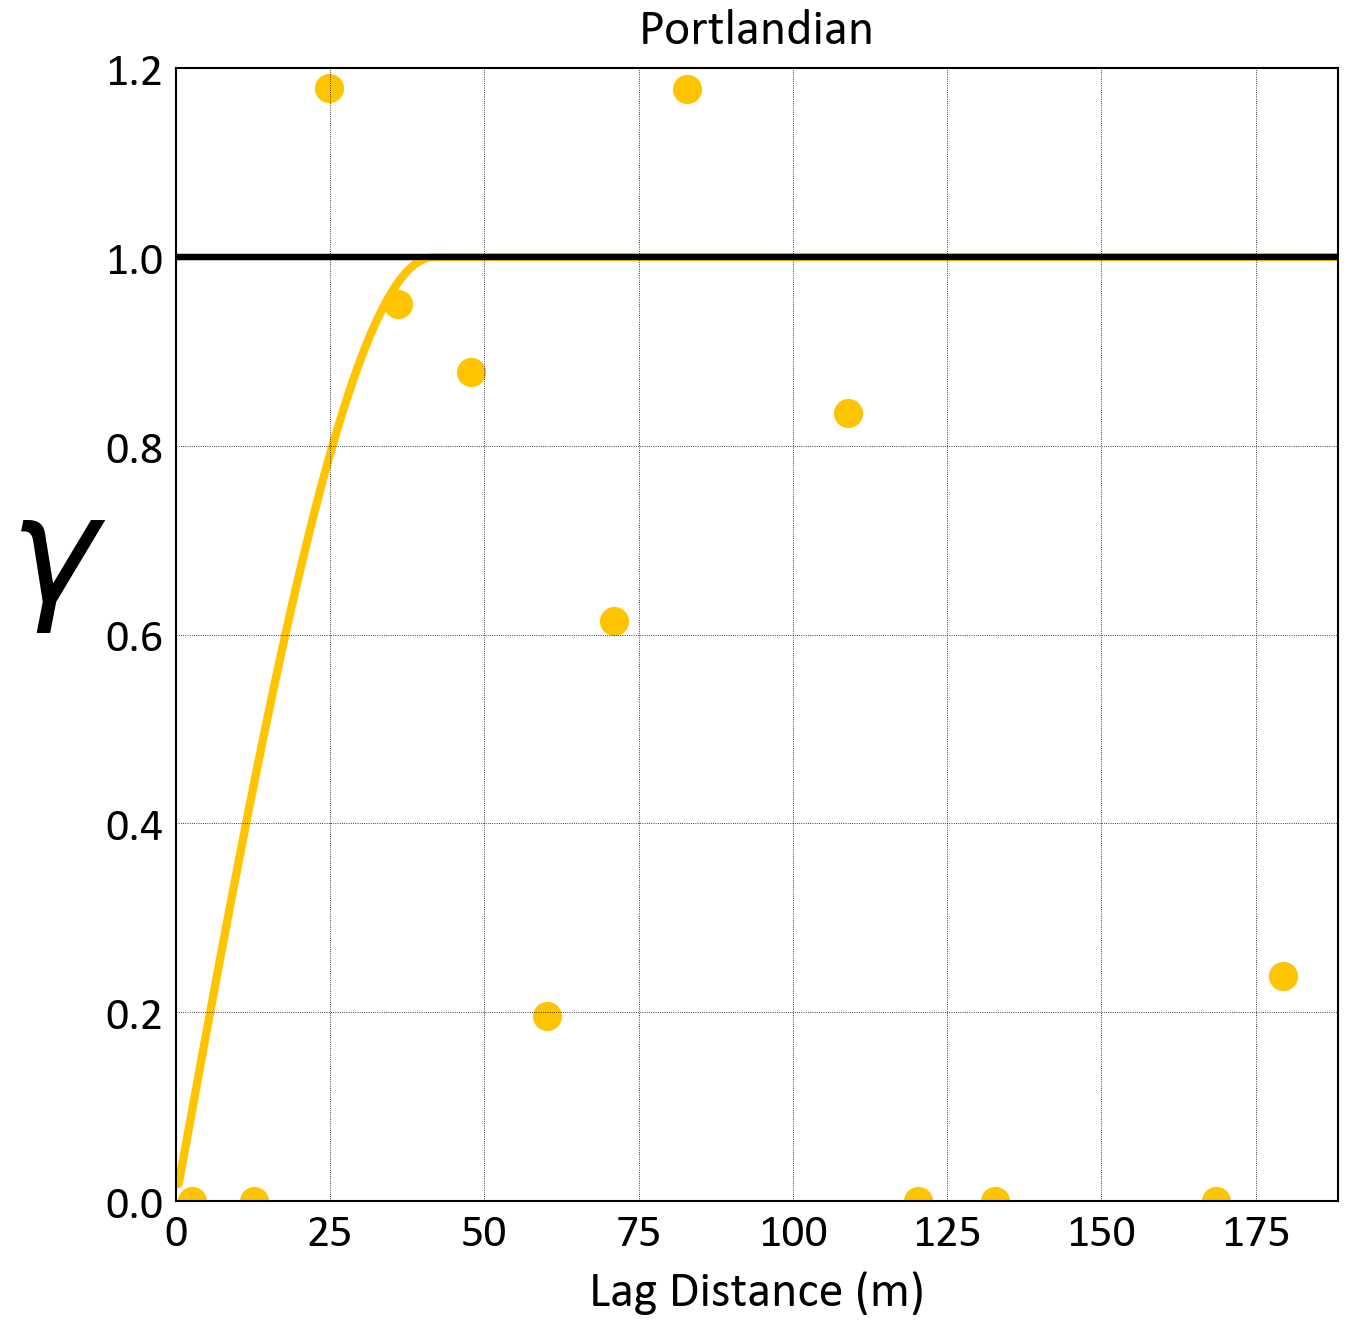
\includegraphics[width=0.45\textwidth]{capitulo_2/imagens/jura_var_4.png}\label{fig:jv4}} \\
    \subfloat[][Quaternary.]{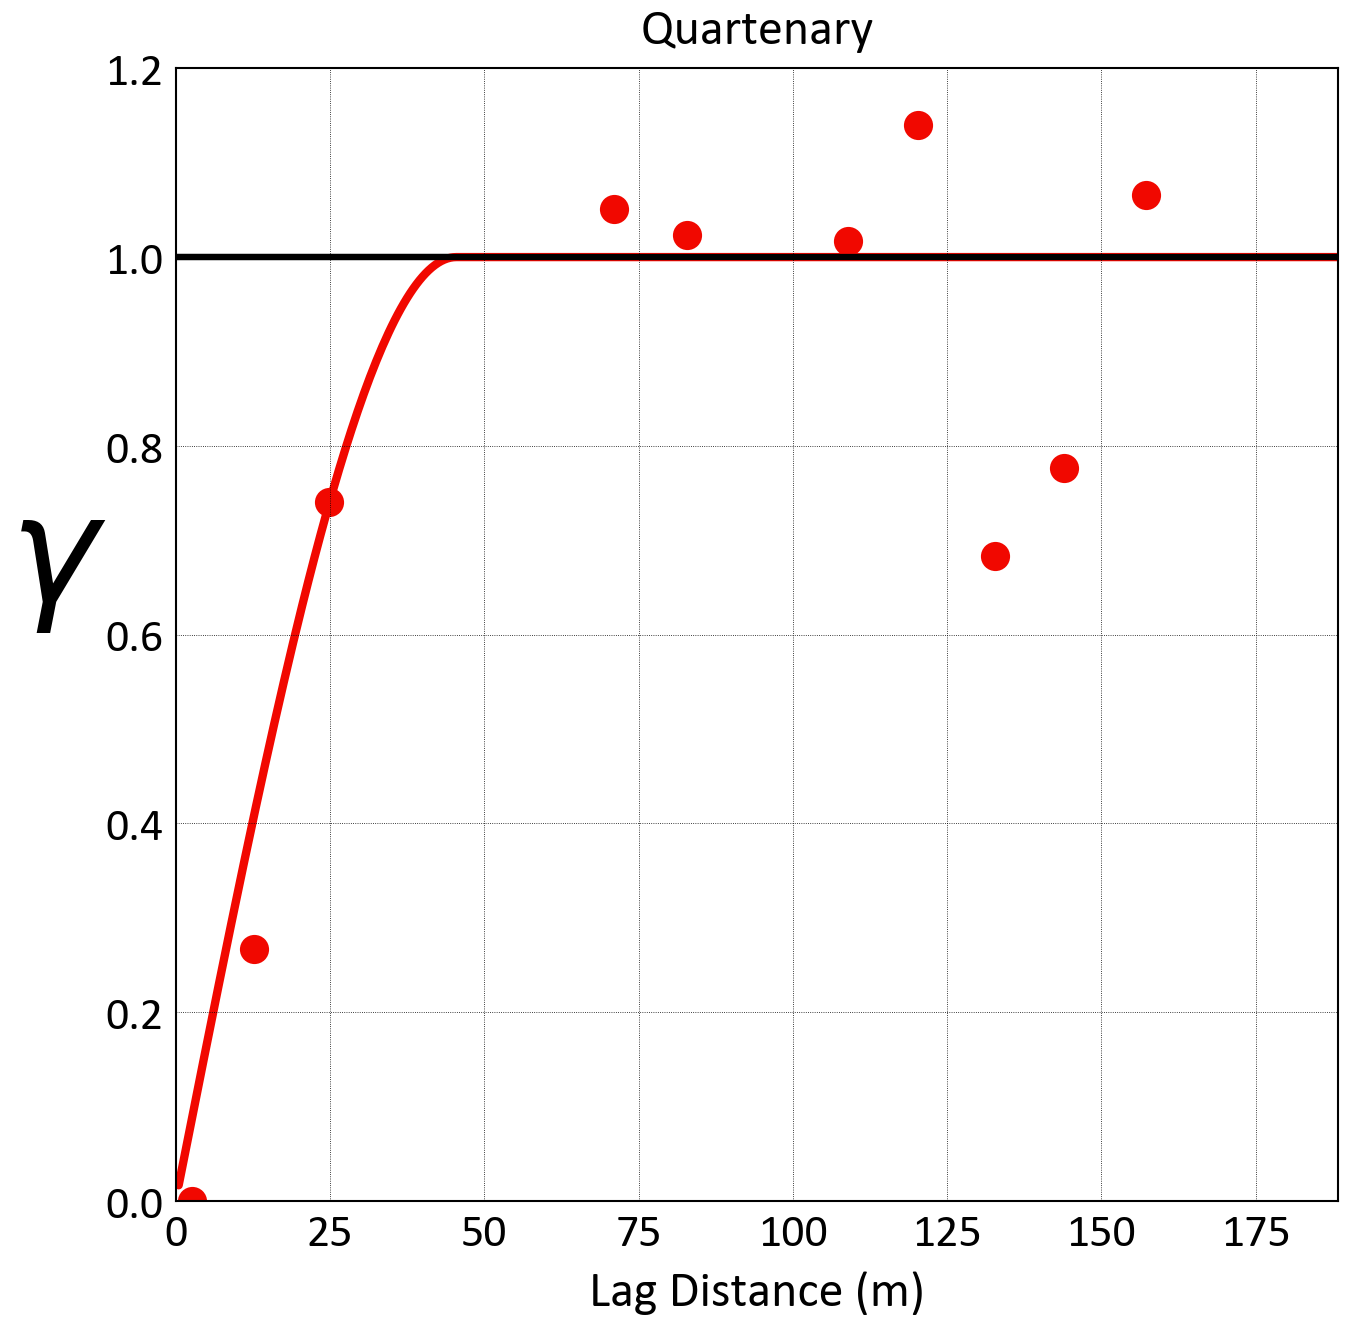
\includegraphics[width=0.45\textwidth]{capitulo_2/imagens/jura_var_5.png}\label{fig:jv5}}
\end{figure}

As equações: \autoref{var_argovian}, \autoref{var_kime}, \autoref{var_sequ}, \autoref{var_port}, \autoref{var_quart} representam os variogramas das cartegorias \textit{Argovian; Kimmeridgian; Sequian;
Portlandian; e Quartenary}, respectivamente.

\begin{equation}
    \label{var_argovian}
    \gamma(h)=1.0Sph_{1} \left[ \frac{OMNI}{76 m} \right]
\end{equation}

\begin{equation}
    \label{var_kime}
    \gamma(h)=1.0Sph_{1} \left[ \frac{OMNI}{72 m} \right]
\end{equation}

\begin{equation}
    \label{var_sequ}
    \gamma(h)=1.0Sph_{1} \left[ \frac{OMNI}{53 m} \right]
\end{equation}

\begin{equation}
    \label{var_port}
    \gamma(h)=1.0Sph_{1} \left[ \frac{OMNI}{41 m} \right]
\end{equation}

\begin{equation}
    \label{var_quart}
    \gamma(h)=1.0Sph_{1} \left[ \frac{OMNI}{45 m} \right]
\end{equation}

\subsubsection{Interpolação}

Uma vez que as distâncias tenham sido calculadas a partir da localização das amostras, o próximo passo é interpolar as propriedades distância assinaladas para o \textit{grid} definido para a modelagem geológica. Embora métodos implícitos não demandem um \textit{grid} - são métodos conhecidos como \textit{gridless} - o objetivo final é preencher o \textit{grid} de estimativas com as categorias correspondentes ou visualizar o modelo através de isosuperfícies. Técnicas de extração de isosuperfícies exigem a função volumétrica definida exaustivamente em um \textit{grid} retilíneo  \cite{martin2017implicitmodeling}.

Para um número constante de amostras, o tempo necessário para interpolação da função volume para todos os nós do \textit{grid} aumenta linearmente com o número de nós. Os parâmetros do \textit{grid} de estimativas, muitas vezes, são determinado por requisitos de engenharia do projeto. Todavia, o \textit{grid} para definição do modelo geológico pode ser diferente do \textit{grid} definido para os modelos numéricos de teores. A consideração mais importante é a capacidade de reproduzir a menor estrutura geológica de interesse.

Considere as seções de um modelo geológico na \autoref{grid_res} gerados em \textit{grids} de diferentes resoluções.

\begin{figure}[H]
	\centering
	\caption{\label{grid_res}Efeito da resolução do \textit{grid} na reprodução de estruturas geológicas.}
	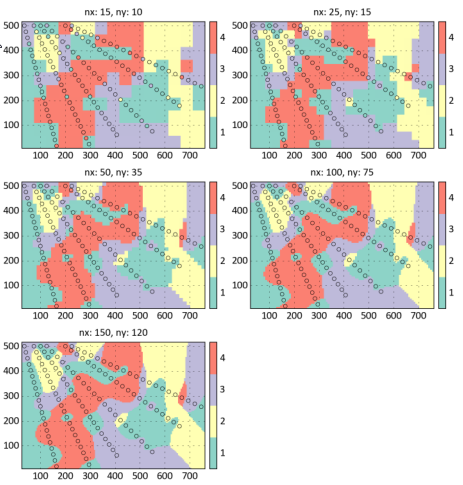
\includegraphics[width=0.6\textwidth]{capitulo_2/imagens/grid_res.png}
	\legend{Fonte: \citeonline{martin2017implicitmodeling}}
\end{figure}

A resolução adequada para esse modelo é entre (nx, ny) = (50, 35) e (nx, ny) = (100, 75). Para os dois primeiros \textit{grids} mais grosseiros há classificação errônea dos nós colocados com amostras, além de (nx, ny) = (100, 75) há pouco benefício na reprodução das estruturas levando em consideração o aumento do tempo de interpolação.

É preciso encontrar um balanço entre resolução e tempo de interpolação. A resolução do \textit{grid} pode ser aumentada a medida que o projeto avança e mais informação é adquirida \cite{martin2017implicitmodeling}.

Qualquer método de interpolação pode ser utilizado, mesmo os métodos do inverso da distância produzem resultados realistas. A krigagem e as funções de bases radiais permitem incorporar informação adicional através dos modelos de covariância parametrizados a partir das amostras.

\citeonline{hosseini_deutsch_iqd} utilizaram inverso da distância, \citeonline{silvaenhancedgeomodeling} utilizou krigagem  global, \citeonline{rolo_dissertacao} utilizou krigagem ordinária, \citeonline{silva_dual} aplicaram krigagem dual. \citeonline{boisvert_geomodeling} gerou modelos implícitos através de distâncias assinaladas com anisotropia variável local (\textit{Locally varying anisotropy kriging - LVA}) e \citeonline{cowan2002rapid} propuseram a utilização de interpoladores baseados em funções de bases radias (\textit{radial basis functions - RBF}), \citeonline{manchuck_MLS} ainda propuseram a utilização de mínimos quadrados móveis para incorporar interpretação manual em seções e avaliar incerteza. A escolha do interpolador deve ser baseada em suas propriedades, na informação exigida para parametrizá-lo (o variograma, por exemplo) e nas sua capacidade de se ajustar a formas geológicas.

Especialmente para as funções distância assinaladas, existe um problema adicional relacionado à estacionariedade de primeira e segunda ordem. Existe uma forte tendência (\textit{trend}) que restringe os estimadores baseados em krigagem para que a estacionariedade seja mantida. Além disso, formas geológicas são curvilíneas e não são bem descritas por funções de covariância "tradicionais" onde a distância euclideana entre os pares de pontos são medidas em linha reta. Por esses motivos muitos autores preferem as funções de bases radiais já que ela não se baseia em estacionariedade de primeira ordem e honram localmente formas geológicas sem a necessidade de parametrização especial \cite{martin2017implicitmodeling}.

Independente do método de interpolação, os modelos gerados devem ser livres de artefatos para que os artefatos do modelo implícito não sejam transferidos para os modelos geológicos. Por esse motivo, interpoladores globais devem ser usados por utilizarem todas as amostras em cada estimativa, já para os métodos baseados em inverso da distância e krigagem (não global) os parâmetros de busca são uma escolha crítica \cite{martin2017implicitmodeling}. Em contrapartida, métodos globais possuem limitações em bancos de dados volumosos por dependerem de muito processamento e memória RAM.

A \autoref{interpsd5} mostra as distâncias assinaladas para a categoria Quaternary do \textit{Swiss Jura} interpolada por krigagem dual (\autoref{dksection}) em um grid 3x3 metros. O variograma dos indicadores da Figura \autoref{fig:jv5} foi usado para para parametrizar o variograma Gaussiano - mesmas estruturas, mesmos ranges, mesmas relações e ângulos de anisotropia.

\begin{figure}[H]
	\centering
	\caption{\label{interpsd5}Categoria Quaternary do \textit{Swiss Jura} interpolada por krigagem dual em um grid 3x3 metros.}
	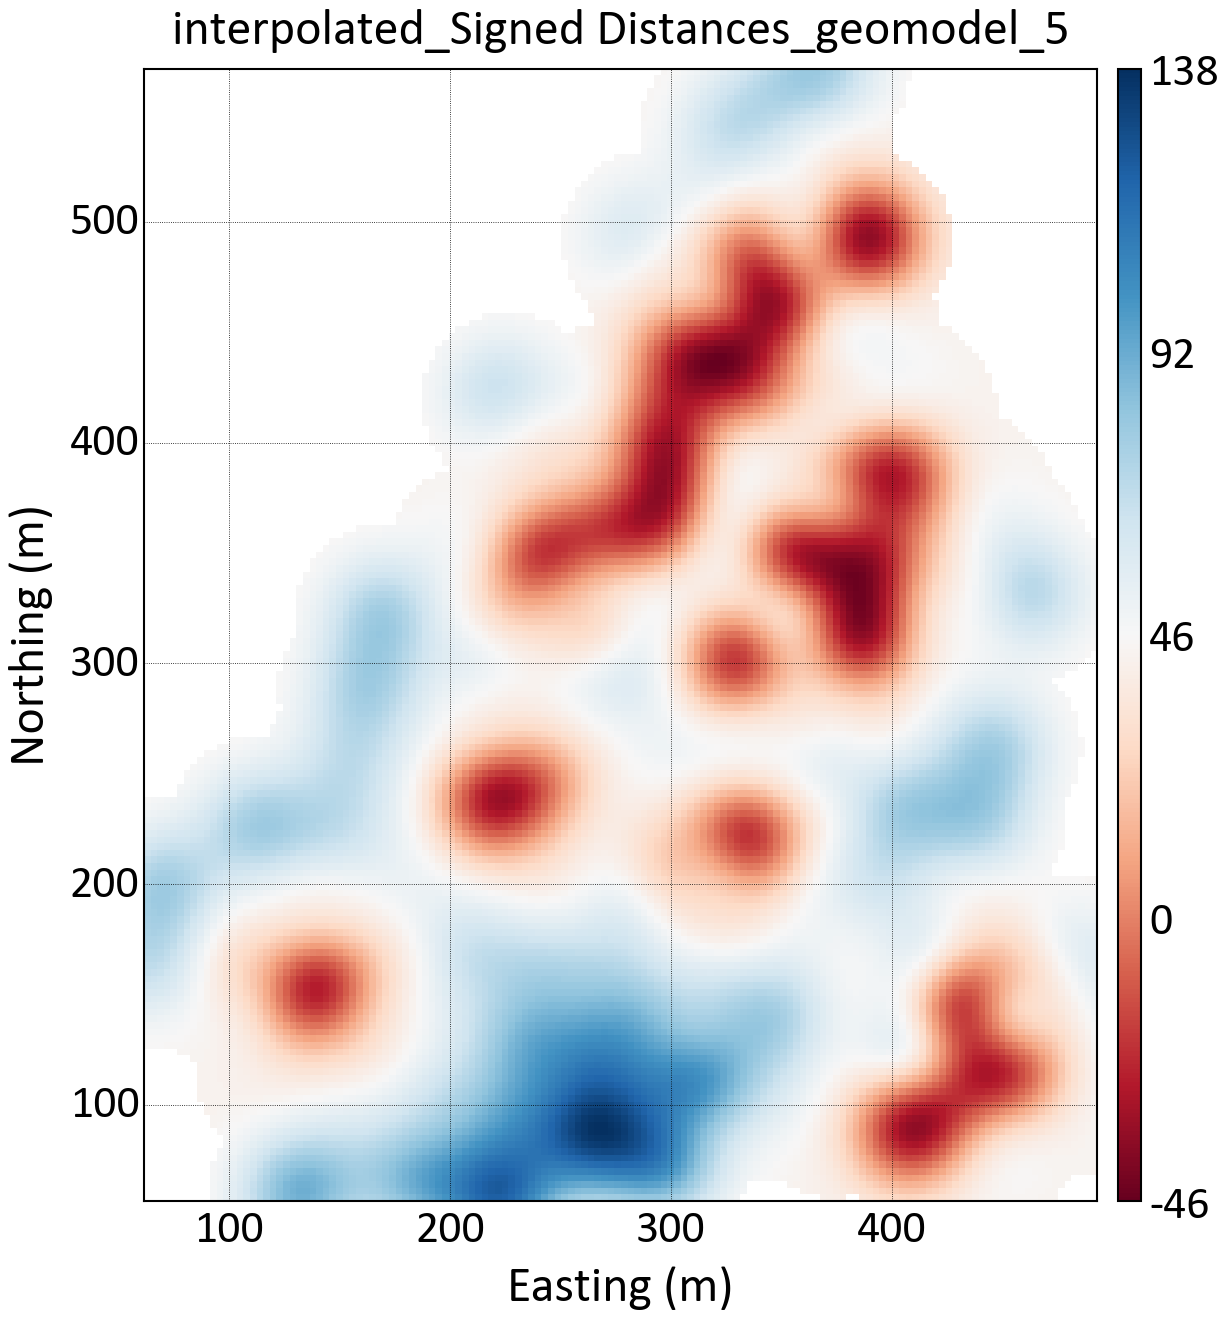
\includegraphics[width=0.6\textwidth]{capitulo_2/imagens/int_sd_5.png}
\end{figure}

Os principais interpoladores globais são listados a seguir.

\subsubsubsection{Krigagem global}

A krigagem global \cite{neufeldglobalkriging} não produz nenhum artefato relacionado à estratégia de busca, porque não há estratégia de busca. O algoritmo lê todos os dados e usa todos os valores dos dados para estimar cada local não amostrado. Um benefício adicional da krigagem global é a redução do tempo de CPU para o cálculo das estimativas já que não é necessário buscar amostras no espaço e a matriz de covariâncias entre as amostras é calculada e invertida uma única vez. O valor estimado da função distância assinalada para um local não amostrado é dado pela \autoref{estimador_k}:

\begin{equation}
\label{estimador_k}
d^*(u)=\sum_{i=1}^{n} \lambda_i(u) d(u_i)
\end{equation}

Onde: $d^*$ é a distância estimada no local não amostrado $u$, $\lambda_i(u)$ é o peso dado para a distância assinalada $d$ observada no local $u_i$.

Os pesos podem ser calculados resolvendo as equações de krigagem. Neste caso, as equações de krigagem ordinária:

\begin{equation}
    \label{global_k}
    \begin{bmatrix}
    C_{11}&\dots&C_{1n}&1\\
    \vdots&\ddots&\vdots&1\\
    C_{n1}&\dots&C_{nn}&1\\
    1&1&1&0
    \end{bmatrix}
    \begin{bmatrix}
    \lambda_{1}\\
    \vdots\\
    \lambda_{n}\\
    \mu
    \end{bmatrix}
    =
    \begin{bmatrix}
    C_{10}\\
    \vdots\\
    C_{n0}\\
    1
    \end{bmatrix}
\end{equation}

Onde $C_{ij}$ é a covariância entre as amostras $i$ e $j$, $C_{i0}$ é a covariância entre a amostra $i$ e o local a ser estimado, $n$ é o número de amostras no dataset e $\mu$ é o operador lagrangeano necessário para a krigagem ordinária \cite{isaaks1989applied}. A condição de não enviesamento é $\sum_{i=1}^{n} \lambda_i=1$.

\subsubsubsection{Krigagem dual} \label{dksection}

A krigagem dual \cite{royer1984dual} é uma representação alternativa da krigagem na qual as estimativas são expressas como uma combinação linear das covariâncias ao invés das amostras. Dessa forma, o estimador da \autoref{dk} torna-se:

\begin{equation}
\label{dk}
d^*(u)=\sum_{i=1}^{n} \omega_i C(u-u_i) + m^*_{OK} \\
\end{equation}

Onde $\omega_i$ é o peso dual associado à covariância $C(u-u_i)$ e $m^*_{OK}$ é uma estimativa da tendência (\textit{trend}). A condição de não enviesamento é $\sum_{i=1}^{n} d_i=0$

Ao contrário da krigagem simples e ordinária o sistema de equações não resulta da minimização da variância do erro, mas sim da propriedade de exatidão do estimador de krigagem.

Os pesos são calculados resolvendo a \autoref{dual_k}:

\begin{equation}
    \label{dual_k}
    \begin{bmatrix}
    C_{11}&\dots&C_{1n}&1\\
    \vdots&\ddots&\vdots&1\\
    C_{n1}&\dots&C_{nn}&1\\
    1&1&1&0
    \end{bmatrix}
    \begin{bmatrix}
    \omega_{1}\\
    \vdots\\
    \omega_{n}\\
    m^*_{OK}
    \end{bmatrix}
    =
    \begin{bmatrix}
    d_{1}\\
    \vdots\\
    d_{n}\\
    0
    \end{bmatrix}
\end{equation}

Onde $d_{n}$ é o valor da amostra da distância assinalada n. $m^*_{OK}$ e $\omega_i$ precisam ser calculados apenas uma única vez e usados para todas as estimativas.

A krigagem dual não necessariamente deve ser global, todavia, sem nenhuma adaptação, seus benefícios só podem ser capitalizados se uma vizinhança global for usada \cite{aunon2000dual}.

\subsubsubsection{Funções de bases radiais (RBF)}

A interpolação com funções de bases radiais \cite{fasshauer2007meshfree} é uma técnica global semelhante à krigagem dual. As RBFs são baseadas no posicionamento de um \textit{kernel} radial em cada ponto amostral. A superfície interpolada é uma combinação linear desses \textit{kernels}. O \textit{kernel} é análogo ao variograma da krigagem. O estimador é descrito pela \autoref{estimador_r}:

\begin{equation}
\label{estimador_r}
d^*(u)=\sum_{i=1}^{n} \lambda_i \theta(u - u_i)
\end{equation}

Onde $\theta$ é o \textit{kernel}, que pode ser parametrizado a partir do variograma dos indicadores para uma determinada categoria, e $\lambda_i$ são os pesos calculados a partir da solução da \autoref{rbf_sist}:

\begin{equation}
    \label{rbf_sist}
    \begin{bmatrix}
    \theta_{11}&\dots&\theta_{1n}\\
    \vdots&\ddots&\vdots\\
    \theta_{n1}&\dots&\theta_{nn}\\
    \end{bmatrix}
    \begin{bmatrix}
    \lambda_{1}\\
    \vdots\\
    \lambda_{n}\\
    \end{bmatrix}
    =
    \begin{bmatrix}
    d_{1}\\
    \vdots\\
    d_{n}\\
    \end{bmatrix}
\end{equation}

$\theta_{ij}$ é o valor do \textit{kernel} entre as amostras $i$ e $j$.

\citeonline{fasshauer2007meshfree} advoga que o \textit{kernel} pode ser parametrizado pela distância que representa a maior esfera que pode ser colocada entre amostras no domínio. Para modelagem geológica, essa técnica tende a super estimar o suporte em relação à parametrização pelo variograma calculado a partir das amostras \cite{martin2017implicitmodeling}.

\subsubsection{Visualização do modelo geológico}

Como as funções distância são negativas no interior do domínio e positivas no exterior, um bom palpite inicial para a interface que separa os domínios no espaço, seria a linha (em duas dimensões) ou superfície (em três dimensões) que corresponda ao valor zero da função distância assinalada \cite{wildedeutschcalibrate}. Dessa forma, blocos em que a distância estimada tem valor negativo, são classificados como pertencentes ao domínio. Blocos em que a distância estimada tem valor positivo, classificados como não pertencentes ao domínio de acordo com a \autoref{classifier}:

\begin{equation}
	i^*(u)=\begin{cases}
	1,\:\textrm{se}\:d^*(u)\leq0\\
	0,\:\textrm{caso contrário}\end{cases}
    \label{classifier}
\end{equation}

A \autoref{quartenary_model} mostra o modelo geológico para a categoria Quaternary do \textit{Swiss Jura}.

\begin{figure}[H]
	\centering
	\caption{\label{quartenary_model}Modelo geológico para a categoria Quaternary do \textit{Swiss Jura}.}
	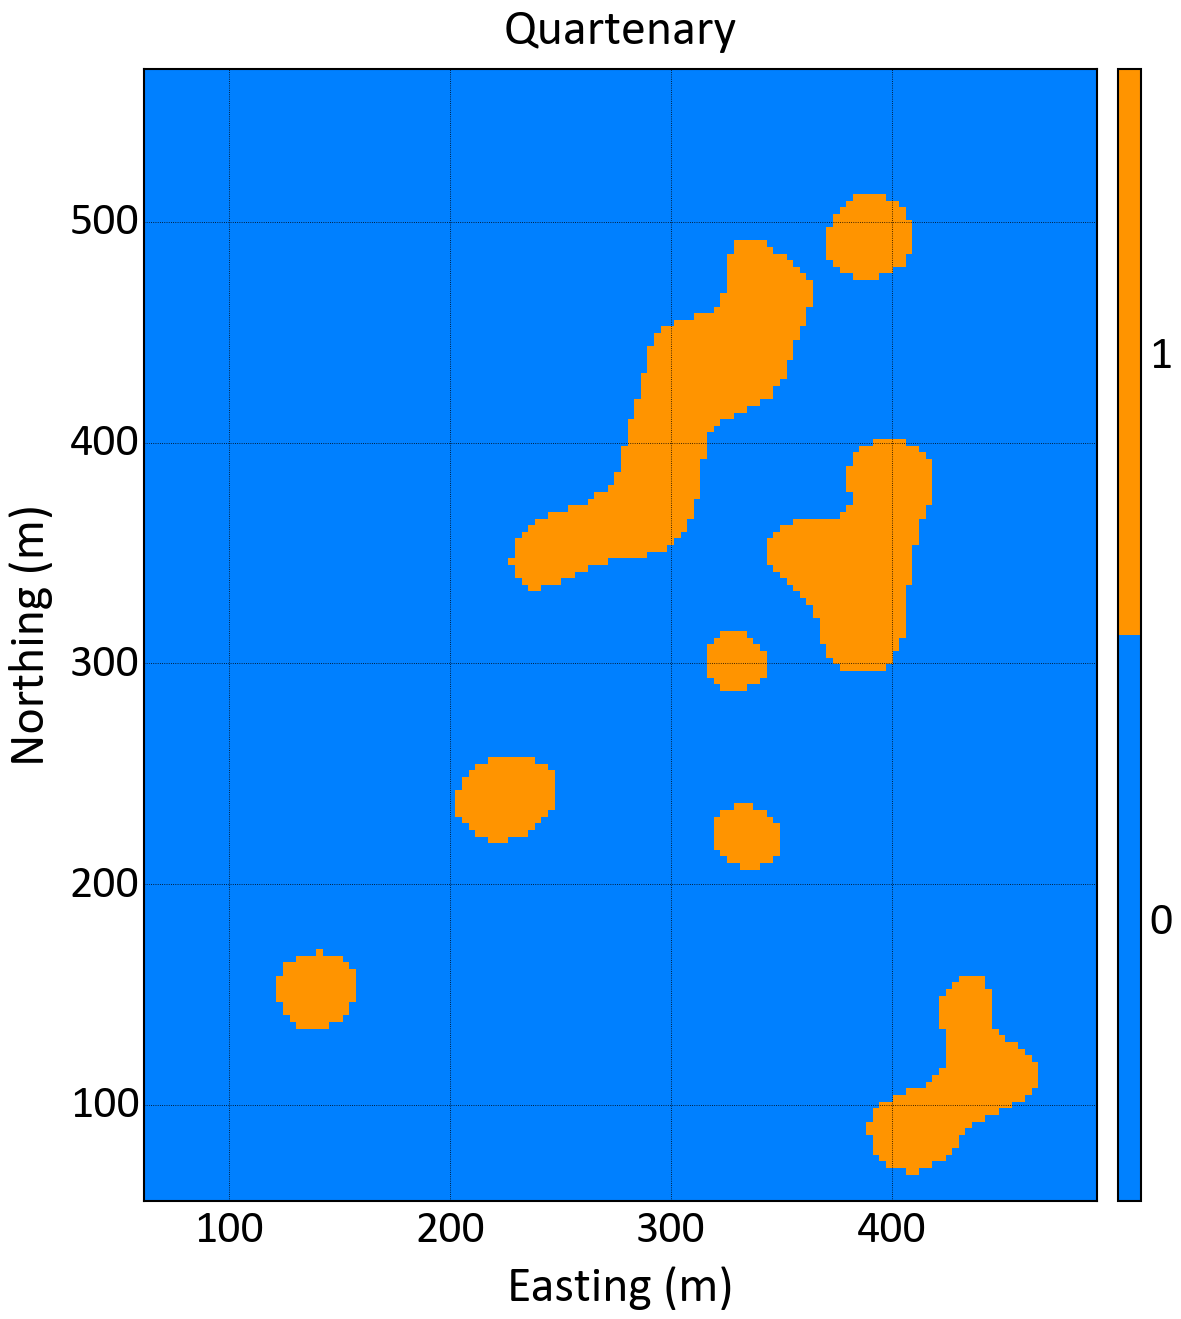
\includegraphics[width=0.6\textwidth]{capitulo_2/imagens/geomodel_quaternary.png}
\end{figure}

A \autoref{one_alt} mostra as coordenadas das distâncias assinaladas estimadas nos eixos x e y e o valor da distância assinalada no eixo z. O plano em cinza corta as distâncias assinaladas na isolinha zero.

\begin{figure}[H]
	\centering
	\caption{\label{one_alt}Uma outra forma de visualizar a modelagem geológica implícita.}
	\subfloat[][Vista 1.]{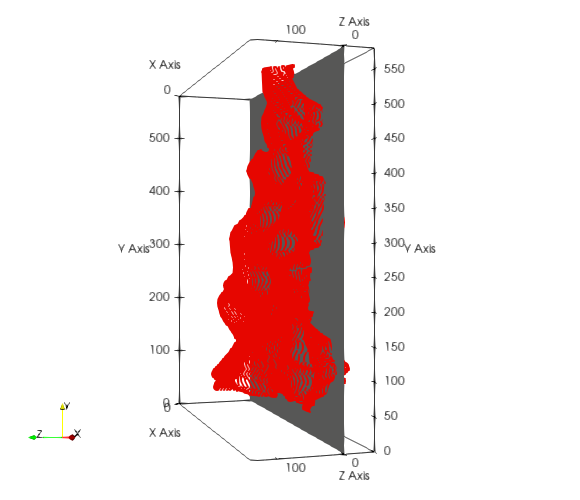
\includegraphics[width=.3\textwidth]{capitulo_2/imagens/one1.png}\label{<figure1>}}
	\hspace{1em}
	\subfloat[][Vista 2.]{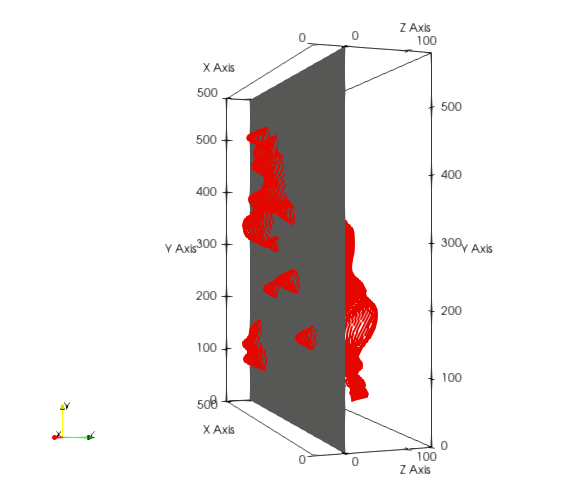
\includegraphics[width=.3\textwidth]{capitulo_2/imagens/one2.png}\label{<figure2>}}
	\hspace{1em}
	\subfloat[][Vista 3.]{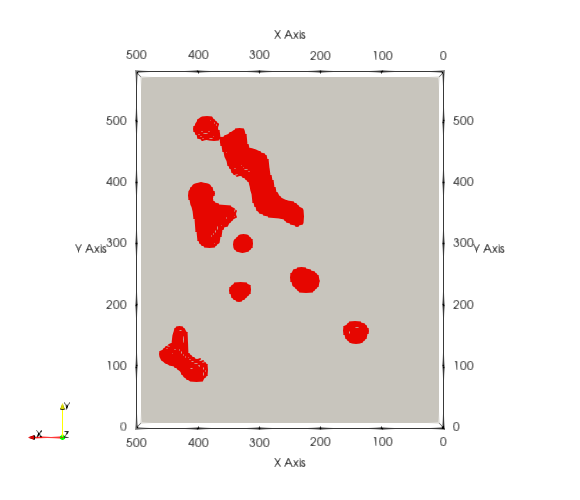
\includegraphics[width=.3\textwidth]{capitulo_2/imagens/one3.png}\label{<figure3>}}
\end{figure}

Em três dimensões um algoritmo de extração de isosuperfícies pode ser aplicado ao modelo implícito para extrair a isosuperfície zero que pode ser posteriormente visualizada como mostrado na \autoref{implicit_3d_ex}. Esse método cria superfícies suaves já que não são delimitadas pelos blocos do \textit{grid} como na \autoref{quartenary_model}.

\begin{figure}[H]
    \caption{Exemplo mostrando a extração da isosuperfície zero e visualização em três dimensões.} \label{implicit_3d_ex}
     \centering
     \subfloat[][Modelo implícito interpolado por RBF para a categoria sendo modelada.]{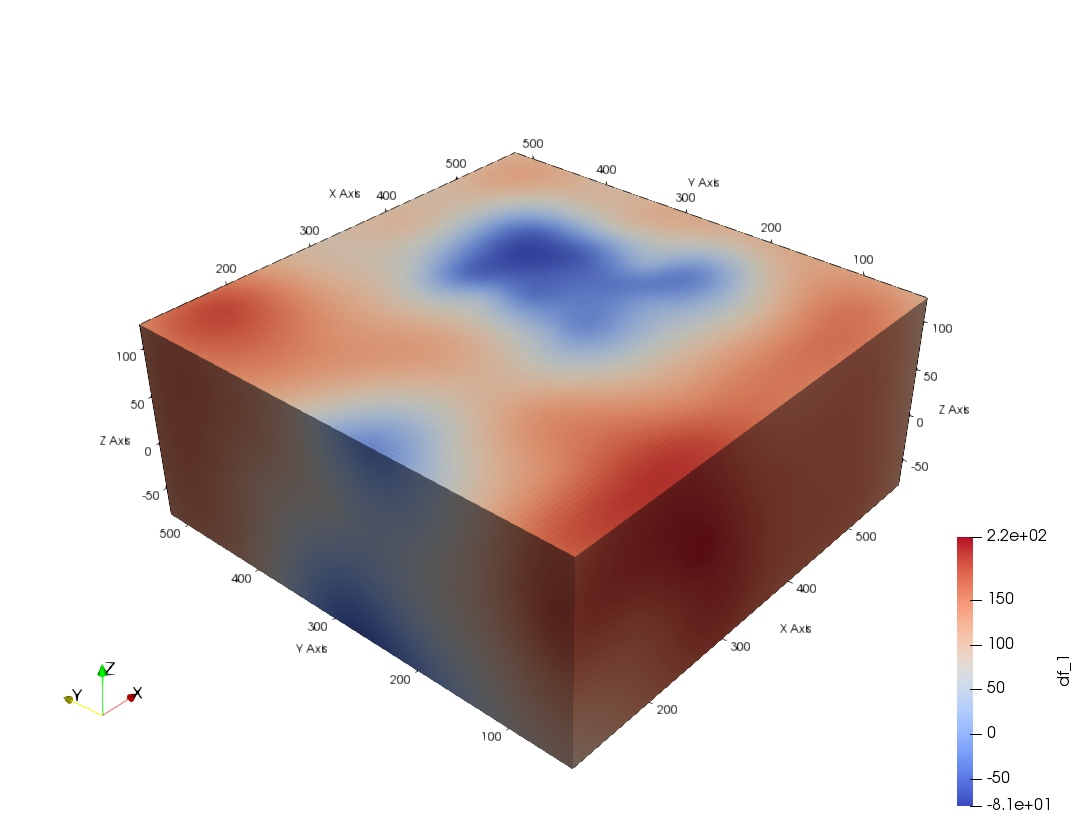
\includegraphics[width=.4\textwidth]{capitulo_2/imagens/rbf.jpeg}\label{fig:c2}}
     \hspace{1em}
     \subfloat[][Isosuperfície zero extraída a partir do modelo implícito.]{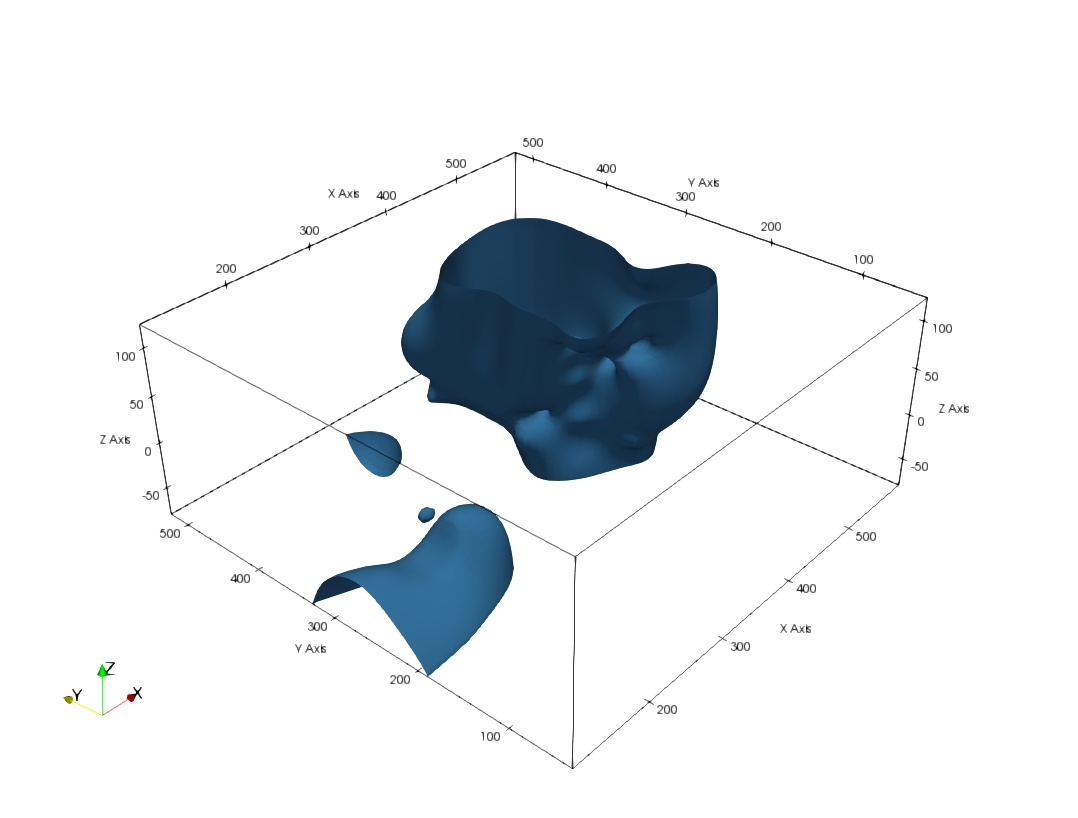
\includegraphics[width=.45\textwidth]{capitulo_2/imagens/isorbf.jpeg}\label{fig:c3}}
\end{figure}

Na presença de múltiplos domínios, as isosuperfícies ou isolinhas, devem ser extraídas uma a uma, e algum tipo de regra hierárquica baseada na idade de cada litologia deve ser aplicada para a criação dos modelos multi-categóricos.

\subsubsection{Adaptação para múltiplas categorias}

\citeonline{silvaanddeutschccgmodeling} propuseram, uma adaptação para o método com o objetivo de modelar múltiplos domínios geológicos simultaneamente, de forma similar ao caso binário.

Se existirem $K$ múltiplos domínios no depósito mineral, para cada ponto amostral ${z(u_\alpha),\alpha=1,...,n}$, um vetor de indicadores de $K$ elementos é codificado de acordo com a \autoref{eq_mult_ind}.

\begin{equation}
	i_k(u_\alpha)=\begin{cases}
	1,\:\textrm{se}\:z(u_\alpha)=k\\
    0,\:\textrm{se}\:z(u_\alpha)\:\textrm{caso contrário}\end{cases} k=1,...,K
    \label{eq_mult_ind}
\end{equation}

A função distância é calculada, individualmente para cada elemento $k$ do vetor, de acordo com a \autoref{eq_mult_sg}.

\begin{equation}
	d_k(u_\alpha)=\begin{cases}
	-\parallel u_\alpha-u_\beta\parallel,\:\textrm{se}\:i_k(u_\alpha)=1\\
	+\parallel u_\alpha-u_\beta\parallel,\:\textrm{se}\:i_k(u_\alpha)=0\end{cases} k=1,...,K
    \label{eq_mult_sg}
\end{equation}

As distâncias calculadas são então interpoladas pelo método escolhido, individualmente para todos os nós do \textit{grid} de acordo com a \autoref{eq_mult_ok}.

\begin{equation}
	d_k^*(u)=\sum\limits_{\alpha=1}^n \lambda_\alpha(u)d_k(u_\alpha)\quad k=1,...,K
    \label{eq_mult_ok}
\end{equation}

Por fim, cada bloco é  classificado pela \autoref{eq_mult_rt}

\begin{equation}
	i^*(u)=k'\;\text{de modo que}\;d_{k'}^*=min\{d_k^*(u)\}_{k=1}^K
    \label{eq_mult_rt}
\end{equation}

As distâncias estimadas fornecem uma medida de proximidade ao domínio oposto mais próximo. Sendo assim, a mínima distância assinalada estimada é tida como o domínio mais provável de ser encontrado numa região não amostrada. A \autoref{eq_mult_rt} sumariza essa ideia \cite{silvaenhancedgeomodeling}. A categoria associada com a menor distância estimada é retida em cada bloco.

A \autoref{multicat_jura} mostra, da esquerda para a direita, as amostras do \textit{Swiss Jura} transformadas em indicadores para cada uma das cinco categorias do depósito, as distâncias assinaladas calculadas para cada uma das propriedades de indicadores, as distâncias estimadas para um grid 3x3 metros por krigagem dual usando equivalentes Gaussianos dos variogramas da \autoref{jura_vargs} e finalmente, o modelo geológico multi-categórico criado a partir da retenção da categoria responsável pela menor distância assinalada estimada em cada local não amostrado.

\begin{figure}[H]
	\centering
	\caption{\label{multicat_jura}Figura esquemática mostrando os passos para a criação do modelo geológico multi-categórico no \textit{Swiss Jura}.}
	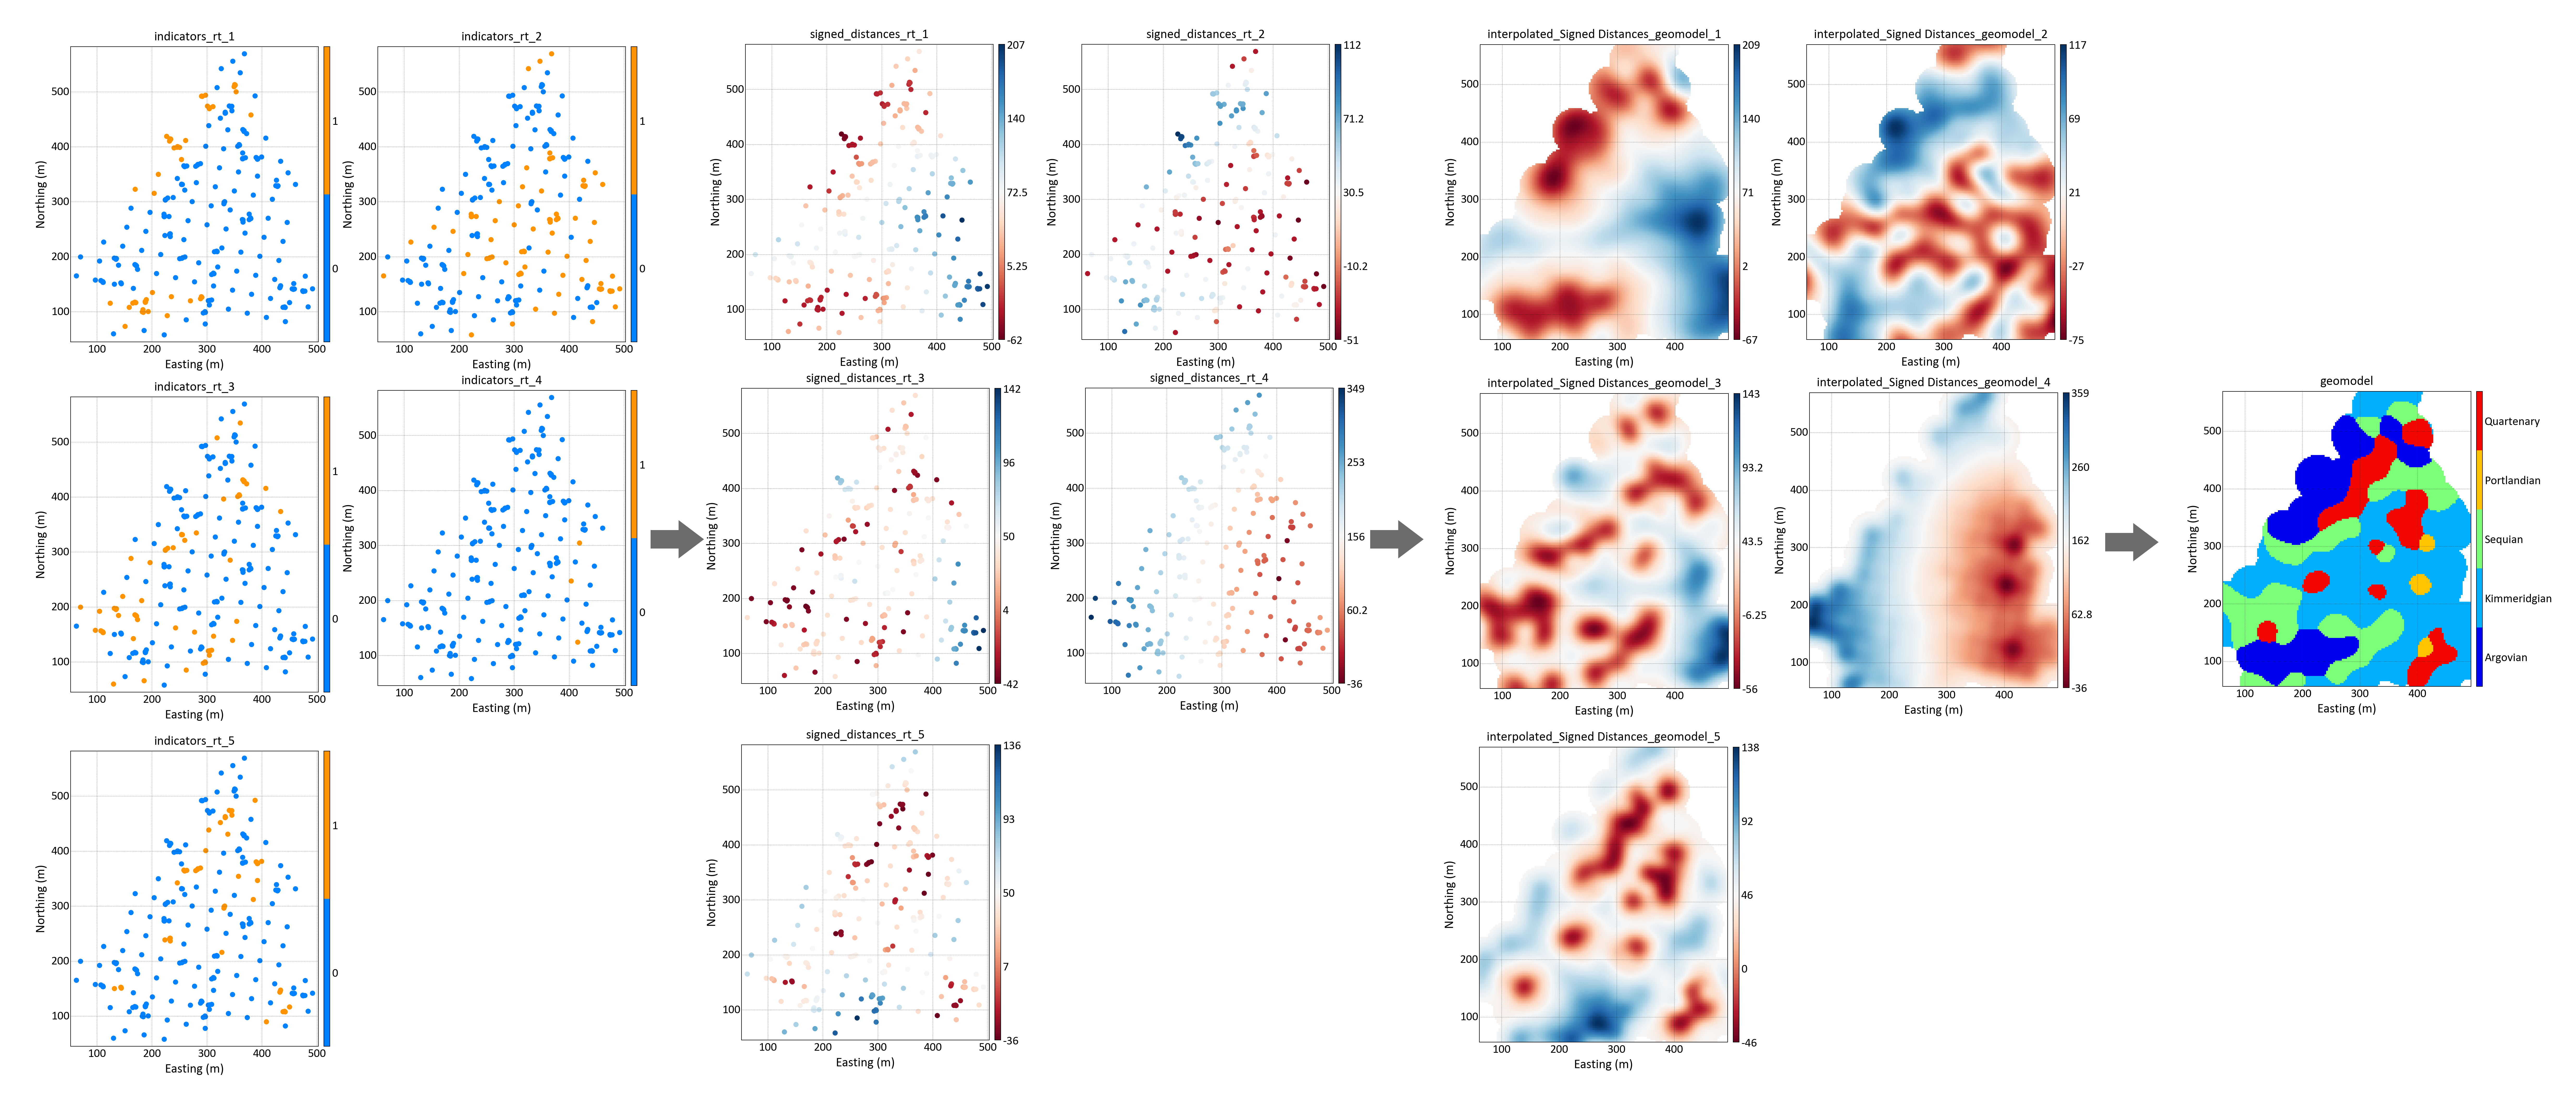
\includegraphics[width=\textwidth]{capitulo_2/imagens/multi category implicit modeling.png}
\end{figure}

A \autoref{multi_alt} mostra as coordenadas das distâncias assinaladas estimadas nos eixos x e y e o valor da distância assinalada no eixo z para cada uma das cinco categorias. Os blocos são classificados com a categoria responsável pela distância estimada "mais negativa".

\begin{figure}[H]
	\centering
	\caption{\label{multi_alt}Uma outra forma de visualizar a modelagem geológica para múltiplas categorias.}
	\subfloat[][Vista 1.]{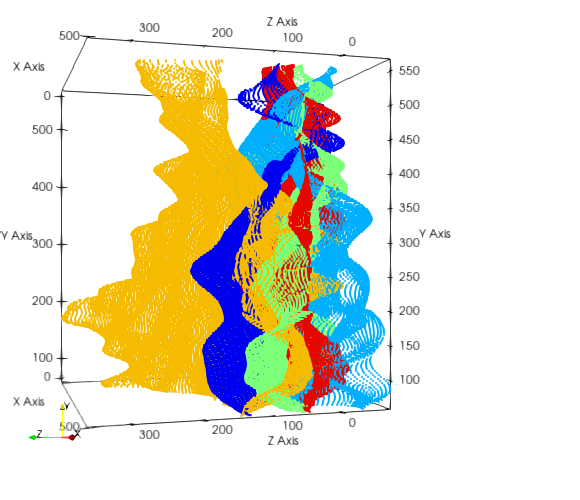
\includegraphics[width=.3\textwidth]{capitulo_2/imagens/multi1.png}\label{<figure1>}}
	\hspace{1em}
	\subfloat[][Vista 2.]{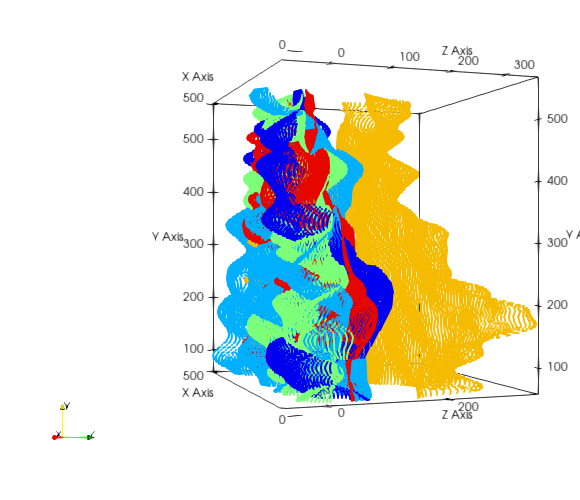
\includegraphics[width=.3\textwidth]{capitulo_2/imagens/multi2.png}\label{<figure2>}}
	\hspace{1em}
	\subfloat[][Vista 3.]{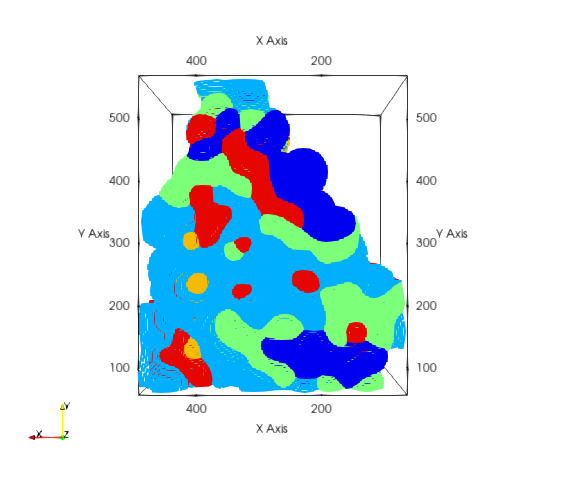
\includegraphics[width=.3\textwidth]{capitulo_2/imagens/multi3.png}\label{<figure3>}}
\end{figure}

\subsubsection{Acelerando o processo}

Embora o uso de métodos globais permita a criação de modelos realistas e livres de artefatos, existem limitações em bancos de dados volumosos já que métodos globais demandam muito processamento e memória RAM. Existem algumas técnicas para superar essa limitação como a solução iterativa \cite{beatson1999fast} por exemplo. Dois métodos que apresentam bons resultados no contexto da modelagem geológica com distâncias assinaladas serão apresentados.

\subsubsubsection{Decomposição do domínio} \label{dom_decomp}

A decomposição do domínio (\textit{Partition of unity - POU}) \cite{wendland2004scattered}, transforma um problema volumoso e que demanda muito esforço computacional em diversos problemas menores e eficientes que são, ao final, unidos.

A demonstração das equações pode ser encontrada em \citeonline{wendland2004scattered} e \citeonline{martin_boisvert_review_rbf}. Um domínio $A$ é subdividido em uma série de partições sobrepostas $\beta$, como mostrado na \autoref{pou} à direita, de modo que a união de todas as $k$ partições em $A$, $\{ \beta \}^K_{j=1}$ compreende o domínio. Para cada partição, os dados correspondentes são utilizados para interpolar a função escalar $s_j(x)$.

A função peso para cada partição deve ser igual a um no centro e 0 na fronteira, a contribuição de cada partição nos locais de sobreposição é dado pela função peso.

As partições são definidas encontrando uma série de coordenadas para seus centros. Diversos métodos podem ser utilizados: um grid regular, k-means, árvore binária, \textit{oct tree}.

A \autoref{pou} mostra um domínio particionado: o particionamento começa considerando o domínio completo como sendo uma partição, então a partição "total"\ é subdividida recursivamente em duas, mantendo um nível de sobreposição. O particionamento termina quando cada partição individual tem menos amostras que o máximo especificado pelo usuário \cite{martin2017implicitmodeling, martin2017iterative}. Dessa forma, áreas com alta densidade amostral ficam em partições pequenas; enquanto, áreas esparsas ocupam partições maiores.

\begin{figure}[H]
	\caption{\label{pou}Particionamento do domínio.}
	\centering
		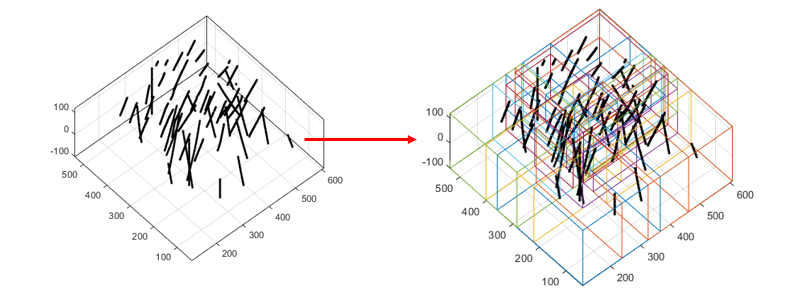
\includegraphics[width=\textwidth]{capitulo_2/imagens/pou.jpg}
	\legend{Fonte: \citeonline{martin2017iterative}}
\end{figure}

Deve haver um número de amostras em cada partição e sobreposição das partições suficientes para evitar o surgimento de artefatos quando as partições independentes forem unidas.

O método deve ser utilizado para um único domínio por vez. Na presença de múltiplos domínios uma regra hierárquica deve ser definida ou a categoria responsável pela menor distância estimada deve ser retida.

\subsubsubsection{Refinamento dos contatos} \label{bound_ref}

\citeonline{silva2015speeding} propuseram uma técnica baseada no algoritmo dos cubos marchantes \cite{lorensen1987marching} para acelerar o processo de modelagem em modelos multi-categóricos. O primeiro passo é criar o modelo geológico usando distâncias assinaladas em um \textit{grid} grosseiro, como mostra o mapa a esquerda na \autoref{refi_cont}.

Depois disso, o algoritmo dos cubos marchantes é aplicado ao modelo geológico com o objetivo de identificar a região ao redor dos contatos. Neste algoritmo, um cubo composto por 8 células em três dimensões ou 4 células em duas dimensões percorre o \textit{grid}, conforme mostrado na \autoref{marcub}, da esquerda para a direita e de cima para baixo visitando todo o \textit{grid}. O algoritmo verifica se pelo menos um dos nós que constituem o cubo pertence a uma categoria diferente dos demais. Nesse caso, esses blocos são marcados como região de contato.

\begin{figure}[H]
\caption{\label{marcub} Esquema mostrando o funcionamento do algoritmo cubos marchantes.}
	\centering
		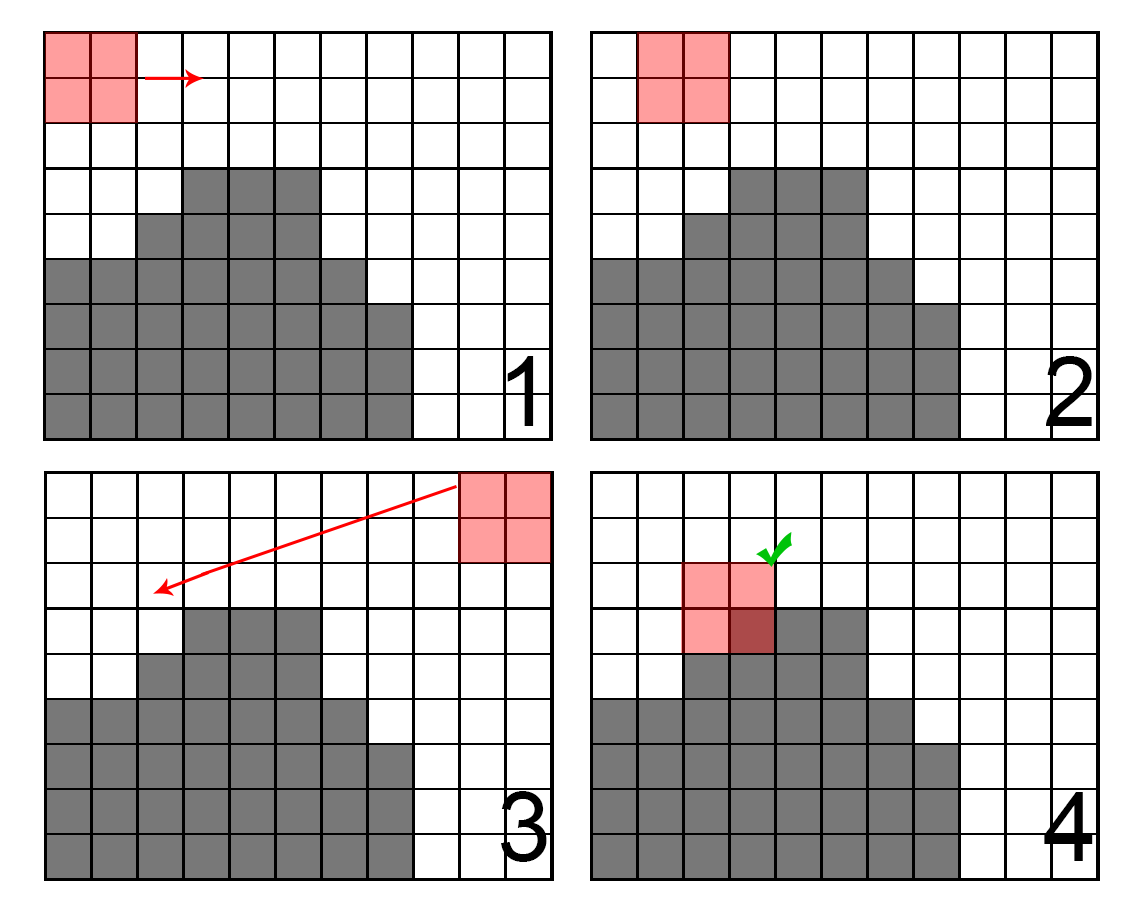
\includegraphics[width=0.6\textwidth]{capitulo_2/imagens/marching_cubes.png}
\end{figure}

Por fim, o \textit{grid} é reduzido (\textit{downscaled}) e uma nova interpolação das distâncias e posterior classificação é realizada apenas nas regiões marcadas como contato. Os demais blocos são classificados com a mesma categoria que pertenciam no modelo no \textit{grid} grosseiro. A posição real do contato necessariamente está localizada na região demarcada pelo algoritmo.

Os passos são repetidos de forma automática, um número de vezes definido pelo usuário, até que a resolução necessária seja atingida.

A \autoref{refi_cont} mostra, seguindo a direção das flechas, o modelo inicial para o \textit{Swiss Jura} criado em um \textit{grid} de dimensões 20x20 m. O algoritmo cubos marchantes então identifica a região dos contatos. Na primeira iteração, as dimensões do \textit{grid} foram reduzidas pela metade, esse parâmetro é escolhido pelo usuário. As distâncias são estimadas no \textit{grid} 10x10 m somente nos blocos marcados como contato pelos cubos marchantes, essa região fica mais estreita a cada iteração. Um novo modelo geológico refinado é criado nesse \textit{grid}. O processo é repetido até que a dimensão dos blocos seja 2.5x2.5 m, como mostrado na imagem da direita na \autoref{refi_cont}.

\begin{figure}[H]
\caption{\label{refi_cont} Esquema mostrando o refinamento dos contatos em três iterações reduzindo as dimensões do \textit{grid} pela metade para o \textit{Swiss Jura}.}
	\centering
		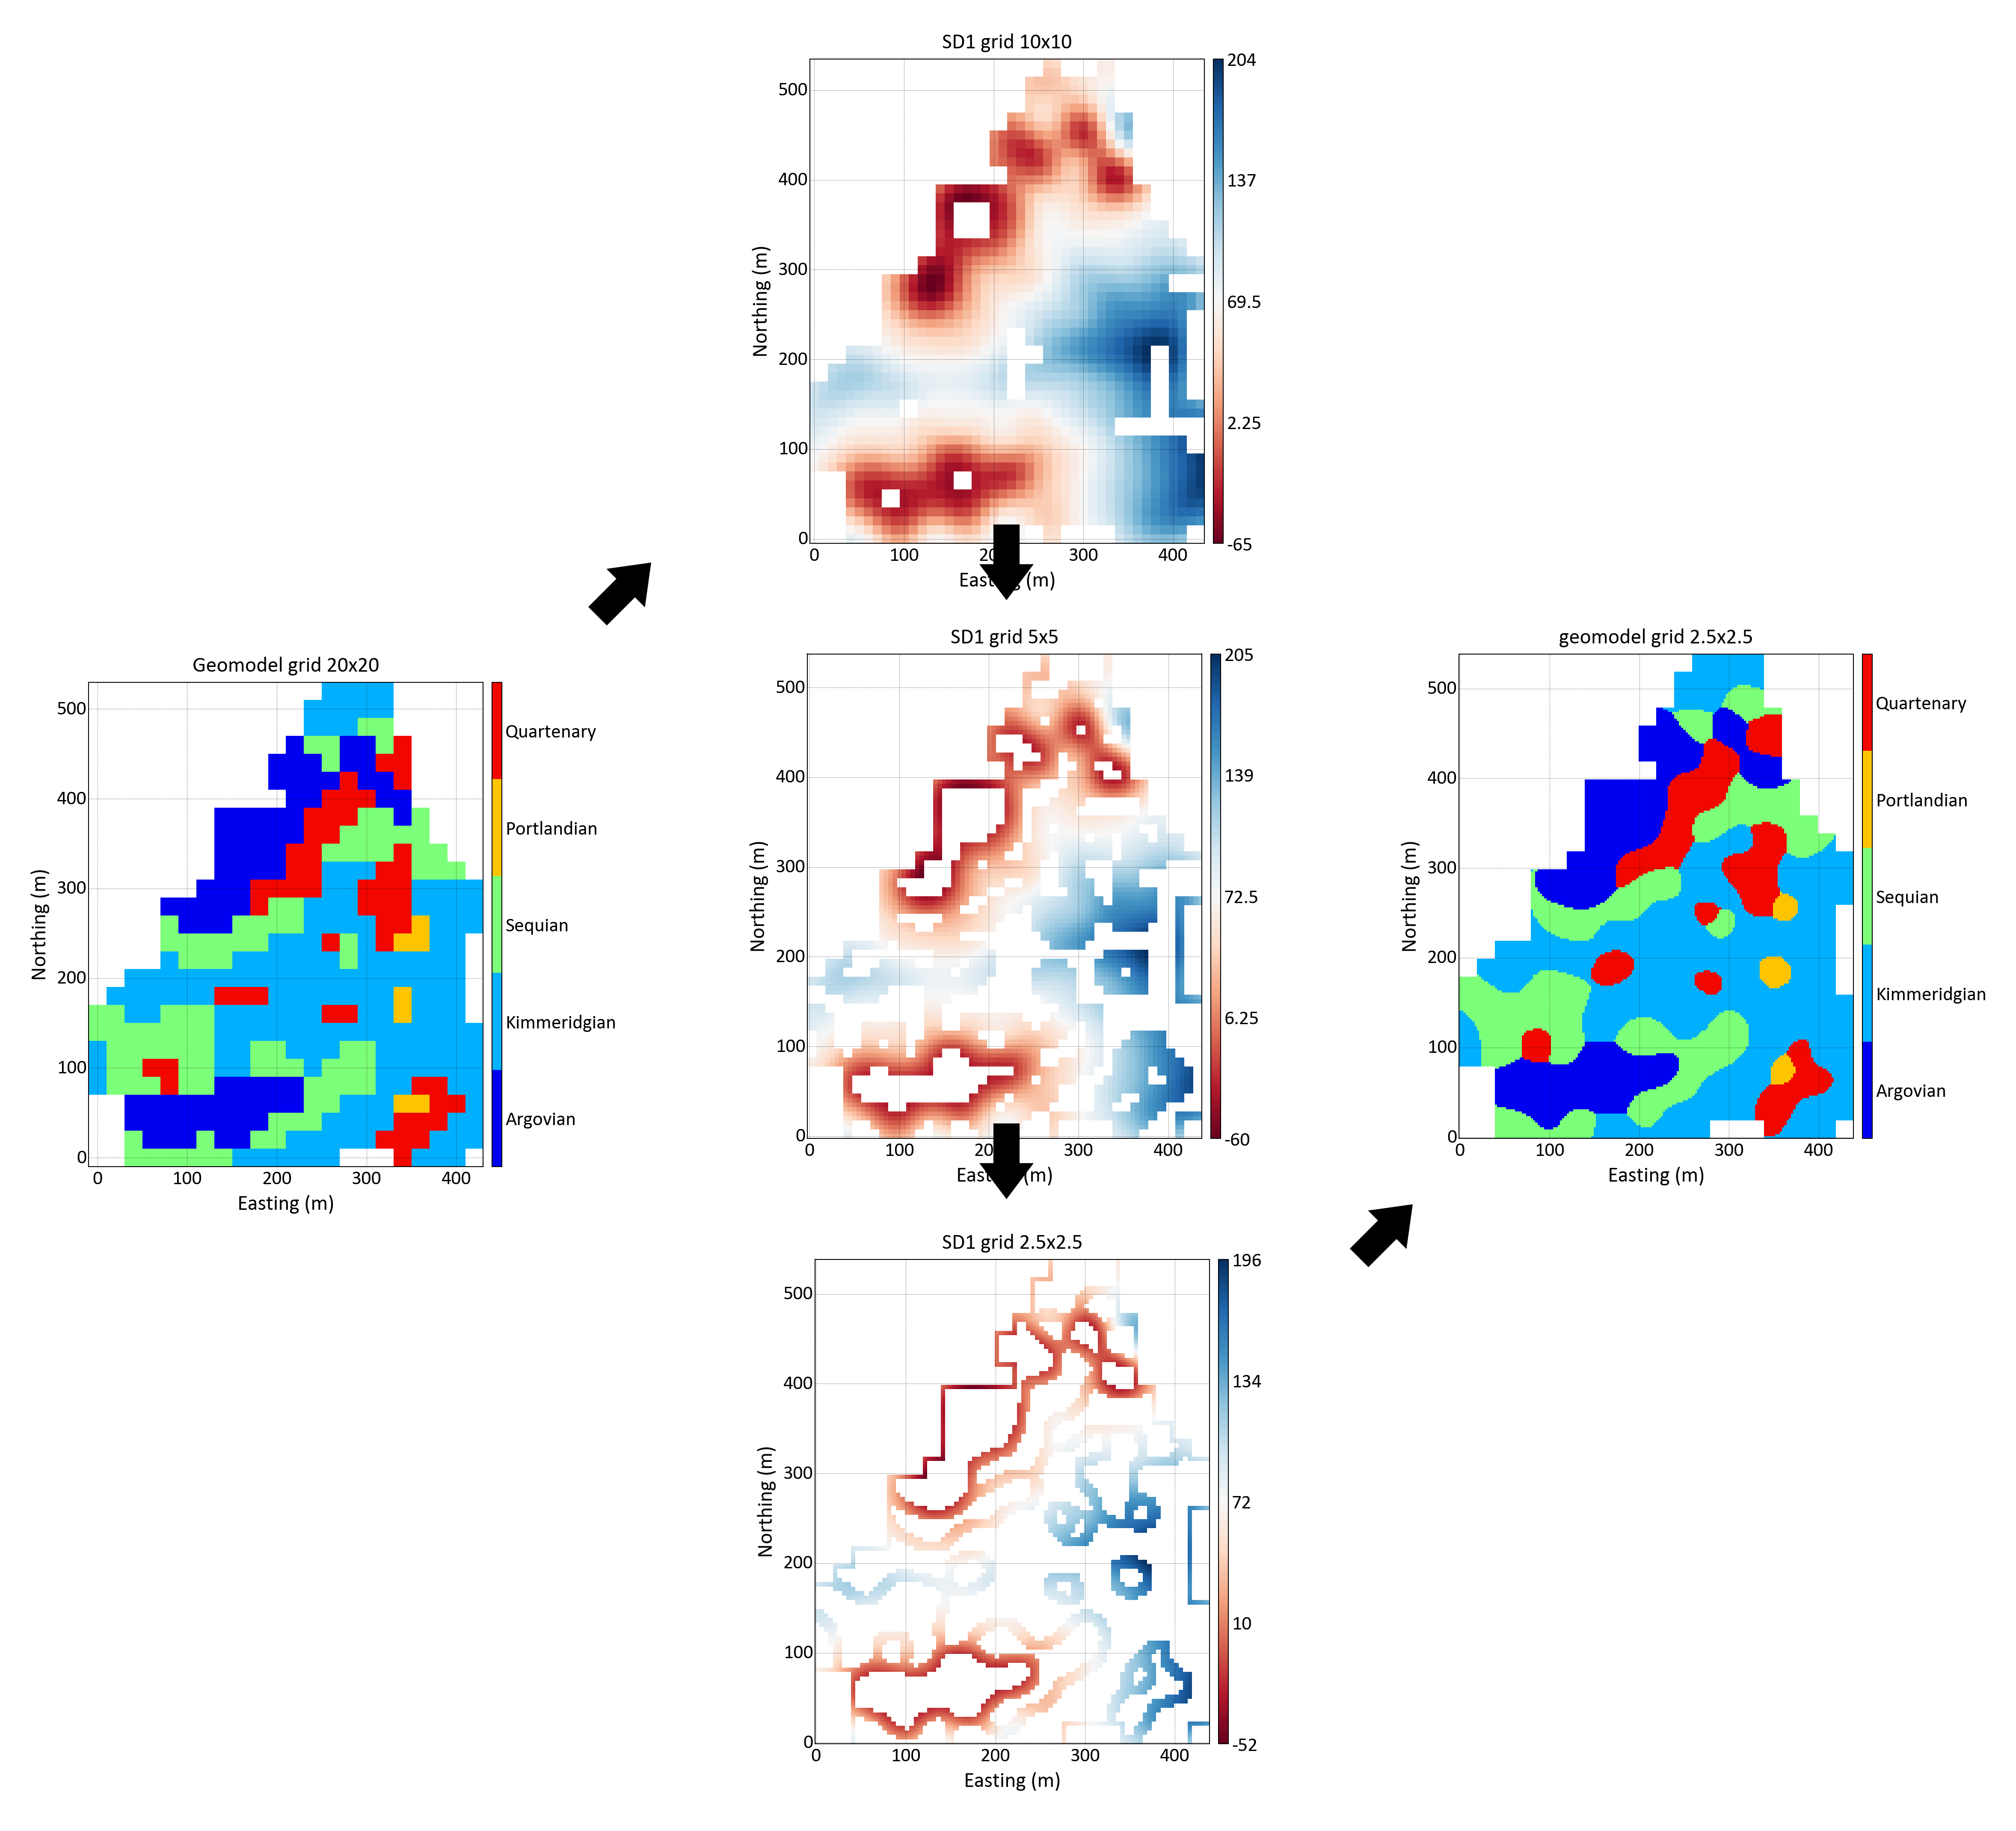
\includegraphics[width=\textwidth]{capitulo_2/imagens/bound_refinement.png}
\end{figure}

\subsubsection{Incorporação de estacionariedade de segunda ordem}

Corpos geológicos são complexos da escala macro à escala micro. Essa característica pode tornar difícil a captura de suas feições com funções de covariância. Segundo \citeonline{martin2017implicitmodeling}, a não estacionariedade de segunda ordem deve ser incorporada quando estruturas complexas estão sendo modeladas.

Anisotropia é definida como o conjunto de rotações e relações anisotrópicas: azimute, mergulho, \textit{rake}, $r1 = \frac{a_{hmin}}{a_{hmax}}$, $r2 = \frac{a_{vert}}{a_{hmax}}$.

\subsubsubsection{Krigagem com anisotropia local variável}

A krigagem com anisotropia variável exige que os parâmetros locais de anisotropia sejam definidos em todos os nós do grid (\autoref{lva_krig_cartoon}), e variem de forma suave pelo domínio. Isso permite que estruturas curvilineares em escala menor que o espaçamento entre as amostras sejam capturadas \cite{martin2017implicitmodeling}. Porém, torna o método computacionalmente exigente.

\begin{figure}[H]
\caption{\label{lva_krig_cartoon}Esquema mostrando os vetores de anisotropia local e as amostras representadas pelos círculos pretos para cada nó do grid.}
	\centering
		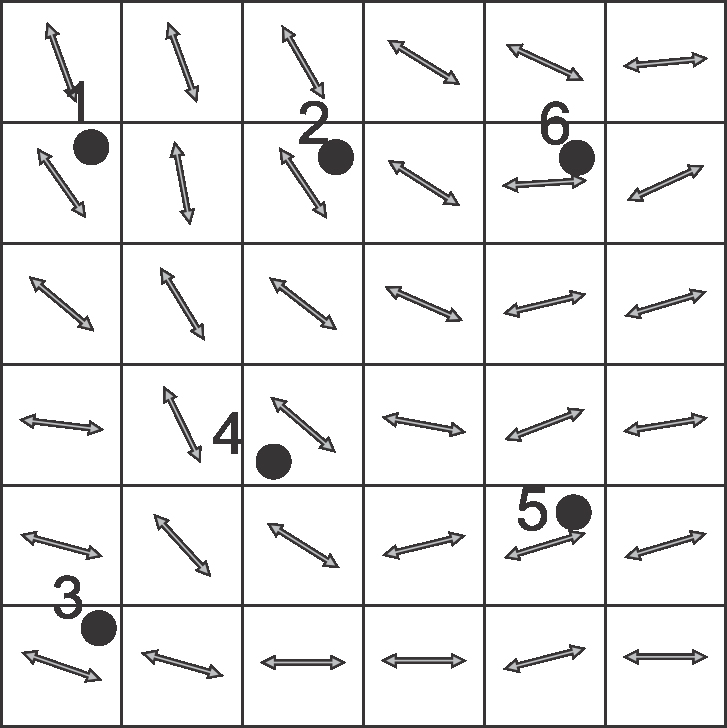
\includegraphics[width=0.6\textwidth]{capitulo_2/imagens/lvakrig.jpg}
	\legend{Fonte: \citeonline{martin2017implicitmodeling}}
\end{figure}

Existem diversos métodos para definição da anisotropia local \cite{lillah2015inference}: pode ser inferida por um geomodelador, estimada diretamente a partir dos dados usando técnicas automáticas, interpolada de uma série de pontos onde a orientação foi medida ou pode ser extraída de dados em um grid que representam a variabilidade local (teores krigados, por exemplo). A biblioteca \textit{GSLib} tem diversos softwares para definição de anisotropia local.

\subsubsubsection{Funções de bases radiais com anisotropia local variável}

Interpolação com funções de bases radiais com anisotropia local variável é baseada na decomposição de domínios (\autoref{dom_decomp}), um kernel anisotrópico pode ser usado para melhor suportar os dados em cada partição, já que as partições são independentes, uma matriz de rotação é usada para definir \textit{kernels} anisotrópicos locais que melhor se ajustam às propriedades espaciais de cada partição. O interpolador de bases radiais é obtido independentemente para cada partição e a solução final é obtida ponderando as soluções independentes nos locais de sobreposição \cite{martin2017implicitmodeling}.

Ao contrário da krigagem com anisotropia local variável, que requer os vetores de anisotropia em todas os nós do \textit{grid}, a implementação para funções de bases radias requer os vetores somente no centro de cada partição (\autoref{lva_krig_cartoon}) variando suavemente pelo domínio.

\begin{figure}[H]
\caption{\label{lva_rbf+cartoon} Esquema mostrando os vetores de anisotropia local e as amostras, representadas pelos círculos pretos, para cada centro de partição representadas pelas linhas tracejadas vermelhas.}
	\centering
		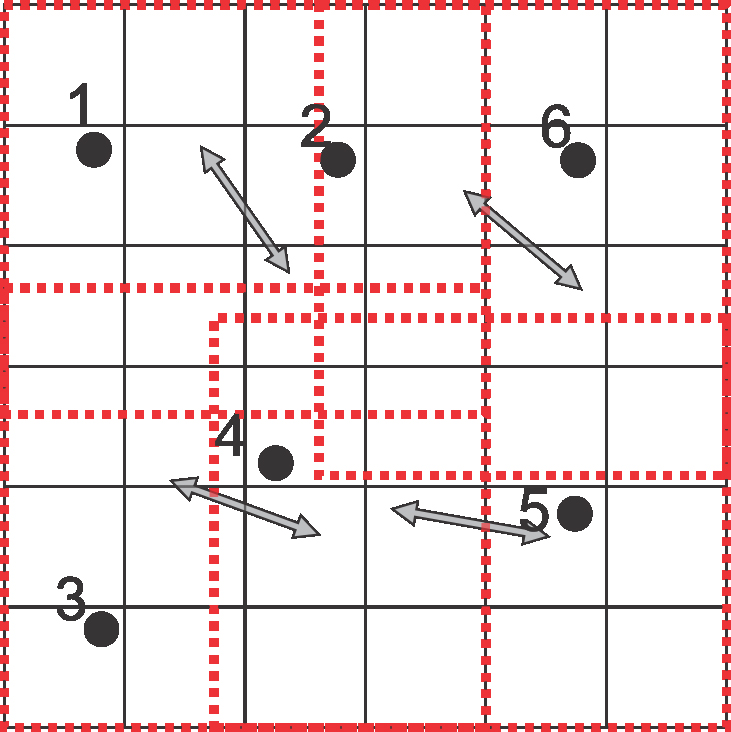
\includegraphics[width=0.6\textwidth]{capitulo_2/imagens/lvarbf.jpg}
	\legend{Fonte: \citeonline{martin2017implicitmodeling}}
\end{figure}

Extrair orientações locais de um modelo criado com anisotropia global e utilizar essas orientações em uma nova interpolação não estacionária resulta em um modelo geológico mais refinado considerando informação local. Esse processo pode ser repetido continuamente refinando o campo de anisotropias locais.

O refinamento iterativo \cite{martin2017iterative} com funções de bases radiais tem um benefício extra (em relação à krigagem com variação local de anisotropia), a possibilidade de incluir algum tipo de critério de parada, quando o modelo for considerado refinado. Como as partições são independentes, se o refinamento de uma partição em particular não resultar em mudanças significativas, poderá ser omitido na solução final. Essa característica torna o processo significativamente mais rápido \cite{martin2017implicitmodeling}.

A \autoref{iterref} mostra um processo de refinamento iterativo onde a semente é um modelo isotrópico. O algoritmo começa sua execução inferindo orientações anisotrópicas em cada flanco da dobra, que são rasos demais para que sejam definidos adequadamente. Porém, nas próximas iterações do refinamento, o mergulho se torna mais profundo e os flancos são definidos implicitamente.

\begin{figure}[H]
\caption{\label{iterref} Esquema mostrando o refinamento iterativo para funções de bases radiais.}
	\centering
		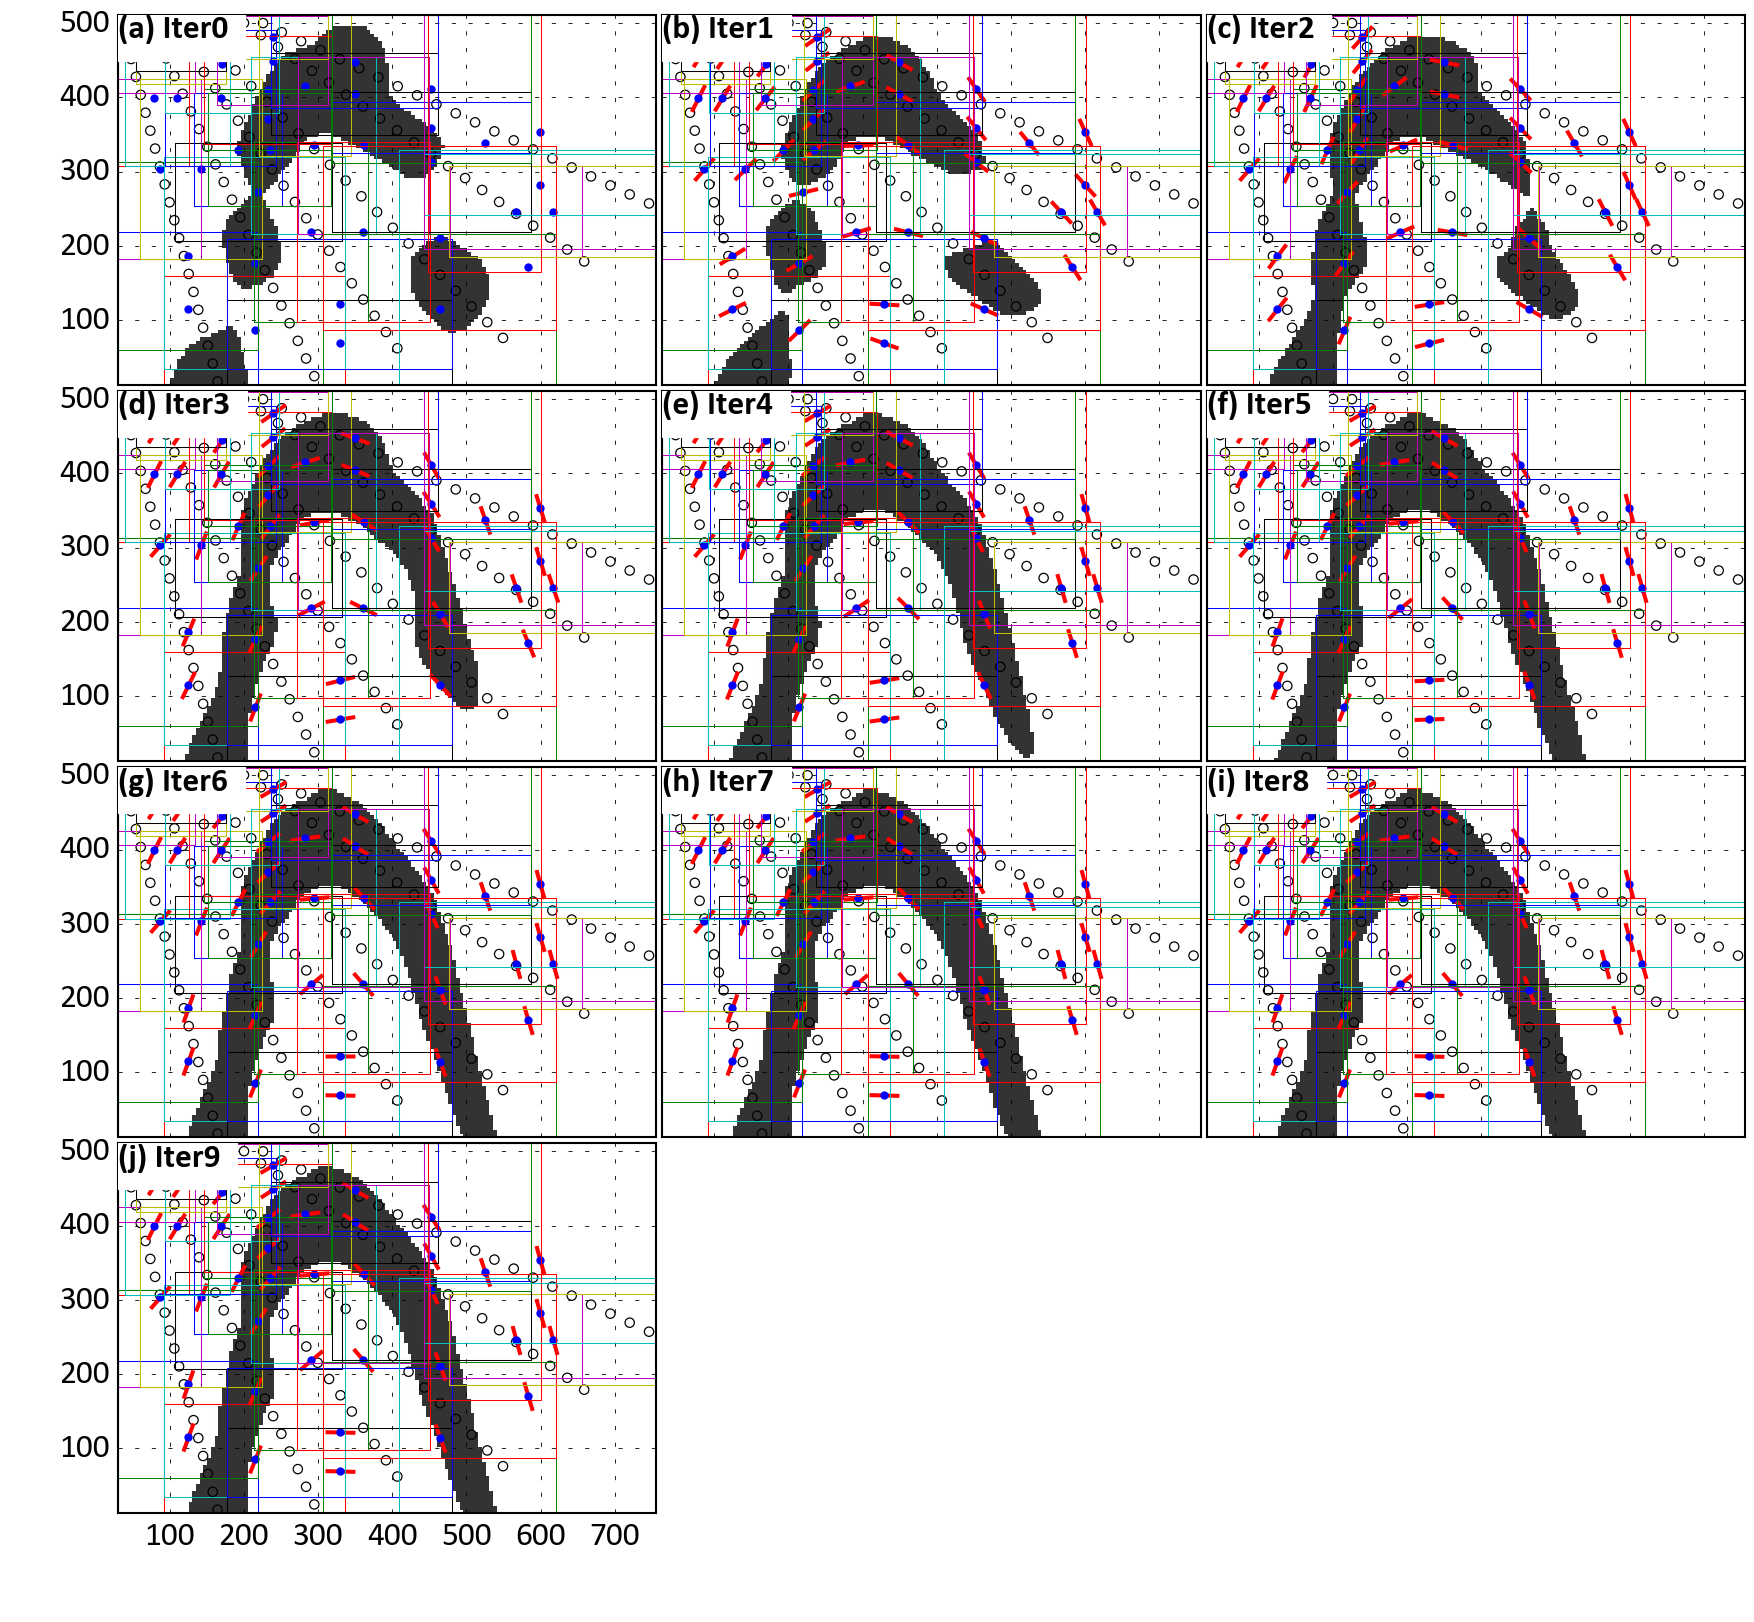
\includegraphics[width=0.6\textwidth]{capitulo_2/imagens/iterref.jpg}
	\legend{Fonte: \citeonline{martin2017iterative}}
\end{figure}

\subsubsection{Desvantagens}\label{problemas}

\citeonline{mancel2019problem} apontam que na presença de dados esparsos e amostras com espaçamento variável, a incerteza em relação à posição dos contatos de um domínio geológico é significativa. Conforme amostras são coletadas e inseridas no modelo, a incerteza em relação à localização diminui e o risco é reduzido. A assimetria espacial na amostragem e a dispersão das amostras são características inerentes às amostragens para avaliação de recursos e podem levar a situações únicas em que as distâncias assinaladas se mostram incapazes de gerar modelos apropriados.

O problema reside no fato do algoritmo para o cálculo da função distância assinalada buscar a amostra mais próxima codificada com um indicador oposto sem levar em consideração a estrutura e o espaçamento dos dados circundantes. Um cenário unidimensional simples ilustra esse viés devido à assimetria na \autoref{desvant1}.

A Figura \autoref{desvant11} mostra a situação ideal, onde a amostra amarela da esquerda aponta para a primeira amostra vermelha, da esquerda para a direita. A primeira amostra vermelha aponta para a amostra amarela da esquerda, assim como a segunda amostra vermelha. Já a terceira amostra vermelha aponta para a amostra amarela da direita, dessa forma, o melhor palpite para o limite (ou a isosuperfície zero) da direita entre os domínios amarelo e vermelho se localiza no ponto médio entre as amostras.

A Figura \autoref{desvant2} mostra a situação que acontece de fato, todas as amostras vermelhas apontam para a amostra amarela da esquerda puxando o limite da direita entre os domínios para perto das amostras vermelhas, diminuindo o tamanho do domínio, ou seja, há um viés conservador no volume dos domínios na presença de forte assimetria nas amostras.

\begin{figure}[H]
    \centering
    \caption{Cenário unidimensional simples ilustrando o viés devido à assimetria nos modelos geológicos.} \label{desvant1}
     \subfloat[][Situação ideal, sem viés.]{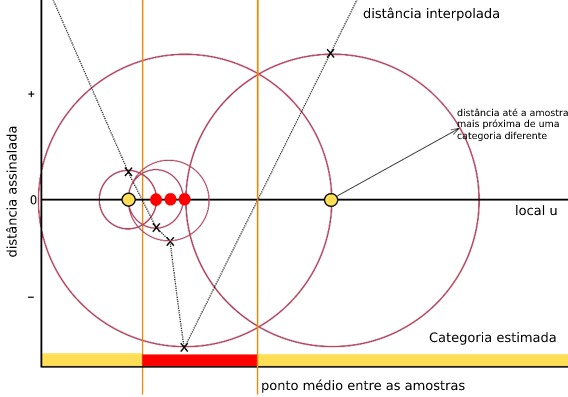
\includegraphics[width=.45\textwidth]{capitulo_2/imagens/sd_prob3.png}\label{desvant11}}
     \hspace{1em}
     \subfloat[][Situação real, com viés conservador.]{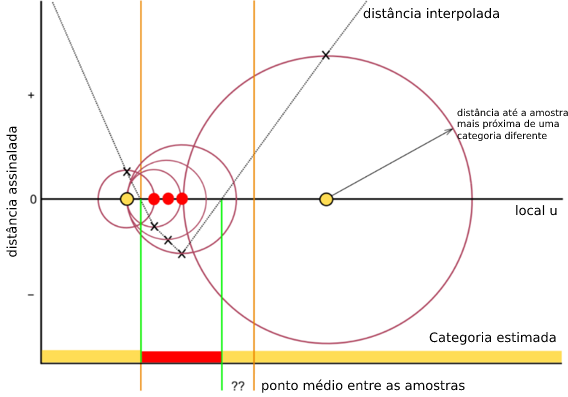
\includegraphics[width=.45\textwidth]{capitulo_2/imagens/sd_prob_2.png}\label{desvant2}}
     \legend{Modificado de \citeonline{mancel2019problem}}
\end{figure}

Os autores propõe uma solução usando indicadores, nesse caso, a isosuperfície definida pela probabilidade de ocorrência 0,5 não é o melhor palpite para a localização do contato. A solução consiste em:

\begin{enumerate}[label=\roman*]
    \item Usar a triangulação de Voronoi para definir a área de influência de cada amostra de indicador;
    \item Calcular a proporção da área total que é ocupada por polígonos que representem amostras do domínio a ser modelado;
    \item Usar a proporção da área (1-p) para definir, a partir da distribuição acumulada da interpolação dos indicadores, o limiar no qual a isosuperfície que represente o contato será extraída. Como mostrado no exemplo da \autoref{nnmet}
\end{enumerate}.

\begin{figure}[H]
\caption{\label{nnmet} Esquema mostrando a extração da iso-superfície usando indicadores e triangulação de Voronoi. À esquerda a figura mostra o CDF dos indicadores interpolados e em vermelho a proporção (1-0.2) ocupada pelos triângulos que representam amostras no interior do domínio que equivale a um valor de indicador de 0.313. À direita um \textit{cutoff} feito em 0.313 nos indicadores interpolados para definir os limites do domínio.}
	\centering
		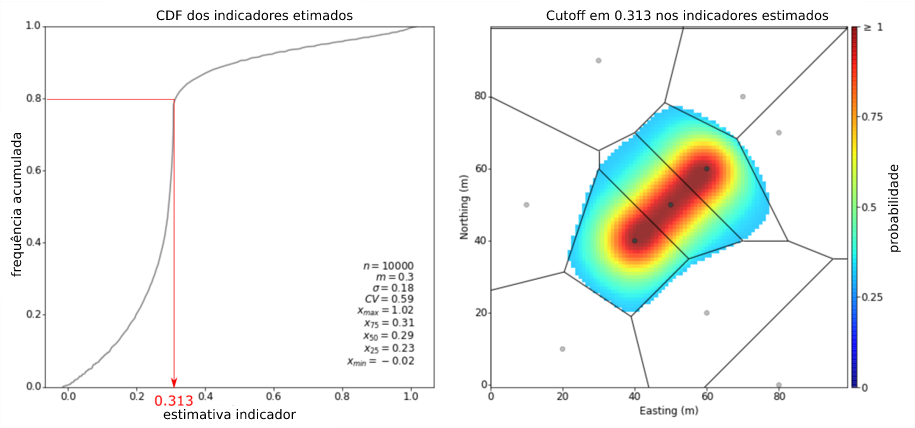
\includegraphics[width=0.8\textwidth]{capitulo_2/imagens/nnmet.png}
	\legend{Modificado de \citeonline{mancel2019problem}}
\end{figure}

\section{Modelagem geológica estocástica}

A necessidade de avaliação da incerteza associada ao modelo geológico impulsionou o desenvolvimento de métodos estocásticos baseados em múltiplas realizações equiprováveis de um atributo. Esses métodos podem ser divididos em dois grupos: métodos baseados em objetos e métodos baseados em células.

\subsection{Métodos baseados em objetos}

Os métodos baseados em objetos \cite{pyrcz2014geostatistical} têm como objetivo a reprodução da morfologia do depósito, como canais meandrantes em um meio fluvial por exemplo. Geralmente os modelos não são condicionados às amostras. Métodos baseados em objetos ainda não têm muita aplicação na mineração encontrando uso na modelagem de reservatórios de óleo e gás.

\subsection{Métodos baseados em células}

Os métodos baseados em células, em contrapartida, são condicionados pelas amostras e são utilizados amplamente pela indústria da mineração.

\subsubsection{Simulação sequencial dos indicadores}

Um dos principais métodos desse grupo é a simulação sequencial dos indicadores \cite{alabert1987stochastic}. O algoritmo é robusto e proporciona uma maneira simples e direta de incorporar a incerteza em modelos geológicos multi-categóricos. Entretanto, os modelos podem apresentar uma aparência ruidosa e não realista do ponto de vista geológico \cite{deutsch2006sequential}.

Seja $F(u;z|(n))$ a distribuição condicional acumulada (ccdf) que modela a incerteza a respeito de $z(u)$ desconhecido. É possível amostrar desse ccdf uma série de L valores simulados $z^{(l)}(u)$. Cada valor representa uma possível realização da variável aleatória $Z(u)$.

A simulação de Monte-Carlo funciona da seguinte maneira \cite{goovaerts1997geostatistics}:

\begin{enumerate}
	\item Uma série de L valores independentes e aleatórios $p^{l}$ uniformemente distribuídos no intervalo [0,1] são amostrados;
	\item O l-ésimo valor simulado $z^{(l)}(u)$ é associado o $p^{l}$-ésimo quantil do ccf.
\end{enumerate}

Da mesma forma que uma série de valores podem ser tomados de um ccdf univariado, um conjunto de mapas simulados $\{z^{(l)}(u'_{j}), j=1,...,N\}, l-1,...,L$ pode ser gerado tomando valores de ccdf N-variado que modela a incerteza conjunta em N locais $u'_{j}$.

Seja  $\{Z(u'_{j}), j=1,...,N\}$ um conjunto de variáveis aleatórias definidas em N locais $u'_{j}$
dentro da área em estudo A. O obejtivo das simulações é gerar diversas realizações conjuntas dessas N variáveis aleatórias. Como mostrado na \autoref{sisim_1}:

\begin{equation}
	\{z^{(l)}(u'_{j}), j=1,...,N\}
	\label{sisim_1}
\end{equation}

Condicionadas ao dados $\{z(u_{\alpha}), \alpha=1,...,n\}$.

Considerando a simulação conjunta de valores em z em apenas dois lugares $u'_{1}$ e  $u'_{2}$. Um conjunto de pares de realizações $\{z^{(l)}(u'_{1}), z^{(l)(u'_{2})}\},l=1,...,L$ pode ser gerado tomando valores do ccdf bivariado. De acordo com a \autoref{sisim_2}:

\begin{equation}
	F(u'_{1}, u'_{2}, z_{1}, z_{2}|(n)) = Prob\{Z(u'_{1})\leq z_{1}, Z(u'_{2})\leq z_{2}|(n)\}
	\label{sisim_2}
\end{equation}

O axioma de Bayes diz que quaisquer ccdfs bivariados podem ser expressos como um produto de ccdfs univariados (\autoref{sisim_3}):

\begin{equation}
	F(u'_{1}, u'_{1}, z_{1}, z_{2}|(n)) = F(u'_{2}, z_{2}|(n+1))F(u'_{1}, z_{1}|(n))
	\label{sisim_3}
\end{equation}

Onde $(n+1)$ denota a condicionalidade aos n valores $Z(u_{\alpha})$ e também à realização $Z(u'_{1})=z^{(l)}(u'_{1})$. A decomposição permite gerar o par $\{z^{(l)}(u'_{1}), z^{(l)}(u'_{2})\}$ em dois passos:

\begin{enumerate}
 	\item O valor $z^{(l)}(u'_{1})$ é tomado do ccdf $F(u'_{1}, z_{1}|(n))$;
 	\item Então o ccdf no lugar $u'_{2}$ é condicionado à realização $z^{(l)}(u'_{1})$ e também as dados, e ao tomar um valor $z^{(l)}(u'_{2})$ desse ccdf, garante-se a correlação.
\end{enumerate}

A ideia aqui é trocar a modelagem e tomada do valor aleatório do ccdf bivariado pela tomada sequencial de valores em dois ccdfs univariados, que são mais facilmente inferidos, daí o nome simulação sequencial.

Esse princípio pode ser generalizado para mais de duas localidades. Aplicando o axioma de Bayes recursivamente, o ccdf N-variado pode ser escrito como o produto de N ccdfs univariados da seguinte forma \cite{goovaerts1997geostatistics}:

\begin{enumerate}
	\item O ccdf no primeiro lugar $(u'_{1})$ é modelado, condicionado aos n dados originais $z(u_{\alpha})$;
	\item Tome desse ccdf uma realização $z^{(l)}(u'_{1})$ que será dado condicionate de todos os ccdfs que serão construídos futuramente;
	\item No i-ésimo nó  $u'_{i}$ visitado, o ccdf será modelado a partir dos n dados originais e também de todos os (i-1) valores $z^{(l)}(u'_{j})$ simulados nos nós $u'_{j}$ já visitados, $j=1,...,i-1$;
	\item Tome desse ccdf uma realização $z^{(l)}(u'_{i})$ que será dado condicionante de todos os ccdfs que serão contruídos futuramente;
	\item Os dois últimos passos são repetidos até que todos os N nós forem visitados.
\end{enumerate}

O conjunto dos valores simulados $z^{(l)}(u'_{j}), j=1,...,N$ representa uma realização da função aleatória $Z(u)$ em todos os nós $u'_{j}$. Qualquer número L de realizações pode ser obtido repetindo o processo L vezes, com diferentes caminhos de visitas aos nós.

Esse processo garante a reprodução do modelo de covariância.

Para simular variáveis categóricas os ccdfs devem ser construídos a partir da krigagem dos indicadores apresentada na \autoref{ik}.

\subsubsection{Simulação geostatística multi-ponto (MPS)}

A simulação sequencial dos indicadores constrói a função de distribuição acumulada $F(u;z|(n))$ a partir da krigagem dos indicadores $i(u_{\alpha}, s_{k})$ em qualquer localização u não medida $I(u;s_{k})$.

Na simulação geoestatística multi-ponto a função de distribuição acumulada é construída na localização u não amostrada através da relação de Bayes \autoref{mps_1}:

\begin{equation}
	Prob(I(u;s_{k})=1|i(u_{\alpha}, s_{k})=1)=\frac{Prob[I(u;s_{k})=1|i(u_{\alpha}, s_{k})=1]]}{Prob[i(u_{\alpha}, s_{k})=1]}
	\label{mps_1}
\end{equation}

Onde, $	Prob(I(u;s_{k})=1|i(u_{\alpha}, s_{k})=1)$ é igual a $[I(u;s_{k})]^{*}_{kst}$ conforme \citeonline{guardiano1993multivariate}.

Essa interpretação probabilística da krigagem simples dos indicadores permite acessar a conectividade espacial de múltiplos pontos pertencentes a um modelo exaustivo (imagem de treinamento), delimitados por um domínio $\tau_{\pi}$ e definidos por n vetores separados $h_{1}, ..., h_{n}$ como mostrado por \citeonline{alves_dissertacao}.

\begin{equation}
	\phi(h_{1}, ..., h_{n};z)=E\{\prod_{\alpha=1}^{n}I(u+h_{\alpha};k)\}
\end{equation}

Onde $\phi(h_{1}, ..., h_{n};z)$ poer lido como a covariância entre múltiplos pontos separados por n vetores $h_{1}, ..., h_{n}$ (os vetores são os limites de$\tau_{\pi}$ ).

A imagem de treinamento (training image - TI) é a ferramenta geoestatística utilizada para capturar a conectividade espacial entre os múltiplos pontos. A TI pode ser definida como um modelo conceitual, que imita os padrões espaciais e estruturais das heterogeneidades presentes em subsuperfície. Geralmente, a modelagem dessas imagens é baseada em afloramentos, imagens de sensoriamento remoto, modelos análogos e interpretação geológica

O processo de varredura da imagem de treinamento é realizado a partir de um template ou vizinhança de busca $\tau_{j}$, composto de um conjunto de j vetores $\{h_j, j=1,...,J\}$ que informa quais pontos da TI serão considerados relevantes em relação a um ponto central  do nó do grid a ser simulado.

Entretanto, como este método exige que a varredura da imagem de treinamento seja realizada para cada nó do grid não amostrado durante a simulação, é demandado de um grande esforço computacional. Como alternativa, \citeonline{strebelle} propôs varrer a imagem de treinamento uma única vez, na qual os padrões da TI são armazenados em um arquivo, denominado árvore de busca ou \textit{search tree}, que possibilita o acesso as informações para cada nó não amostrado simulado \cite{amarante_dissertacao}.

\citeonline{boucher2014simulation} declaram que aplicar MPS a objetos não repetitivos e de grande volume como são os deposites minerais é difícil porque a maioria dos algoritmos de MPS são baseados em repetições de padrões para a simulação. Por esse motivo, os autores propõe um algoritmo focado em reproduzir padrões dos contatos entre as litologias. O algoritmo aprende os padrões a partir dos contatos interpretados por um geomodelador. Uma zona de incerteza ao redor dos contatos deve ser definida.

\subsubsection{Métodos Gaussianos truncados}

Há ainda a família dos métodos Gaussianos truncados. Esses métodos são aplicados, geralmente, quando as litologias ocorrem em uma ordem fixa, como em sequências estratigráficas por exemplo. A ideia básica por trás da simulação Gaussiana truncada \cite{matheron1987conditional} é simular uma variável Gaussiana (contínua) em cada célula do \textit{grid} e então aplicar uma regra de truncagem para converter os valores Gaussianos contínuos em valores categóricos.

A regra de truncagem é uma pare importante dos métodos Gaussianos truncados já que controla os contatos entre as diferentes litologias, suas transições e proporções. A definição da regra de truncagem é geralmente baseada nas probabilidades de transição observadas nos dados e em modelos geológicos conceituais \cite{silva2018enhanced}. Entretanto, diversas técnicas foram propostas para a definição das regras de truncagem.

Em muitos casos, a abordagem Gaussiana truncada se mostra bastante restritiva. Por esse motivo, a técnica pode ser estendida para duas ou mais variáveis Gaussianas. Essa adaptação é chamada de simulação pluri-Gaussiana truncada \cite{armstrong2011plurigaussian}.

O conceito de usar a regra de truncagem em mais de uma dimensão para transformar múltiplas variáveis Gaussianas em uma única variável categórica é limitada, já que a interpretação geológica se degrada quando um número maior de categorias e/ou variáveis gaussianas são consideradas devido à complexidade do modelo.

Por isso, uma nova adaptação foi desenvolvida: \citeonline{silva2019multivariate} propuseram a simulação pluri-Gaussiana truncada hierárquica. Esse método utiliza uma estrutura em árvore para definir diferentes regras de truncagem em uma única dimensão. Isso facilita a definição do mapeamento entre espaço contínuo (Gaussiano) e categórico, tornando possível a utilização eficiente de qualquer número de variáveis Gaussianas para a modelagem de uma variável categórica.

\subsubsection{Métodos implícitos}

No braço dos métodos implícitos, alguns autores desenvolveram técnicas para avaliar a incerteza dos modelos geológicos. Avaliar a incerteza em relação à posição dos contatos a partir dos campos potenciais é uma  processo direto. \citeonline{gonccalves2017machine} deram uma abordagem de aprendizagem de máquinas para o método possibilitando a avaliação de incerteza. \citeonline{de2019gempy} desenvolveram uma ferramenta de modelagem geológica estocástica de código aberto que avalia a incerteza usando campos potenciais combinados com uma abordagem Bayesiana.

Outros autores construíram modelos implícitos e avaliaram a incerteza do modelo geológico usando dados estruturais. \citeonline{lindsay2012locating} examinaram a incerteza introduzida pelos dados de orientação geológica, produzindo um conjunto de modelos 3D implícitos gerados a partir de medições de orientação sujeitas a simulações de incerteza. \citeonline{pakyuz2018monte} estudaram o efeito da propagação da incerteza dos dados estruturais de entrada na modelagem geológica 3D implícita. \citeonline{caumon2007elements} avaliaram a incerteza do modelo geológico ao perturbar os parâmetros geológicos, como superfícies de falha e horizonte de alteração.

Também existem na literatura métodos de avaliação de incerteza baseados em distâncias assinaladas, as próximas seções apresentam os principais. Alguns desses, que são base para alguns dos métodos propostos no \autoref{chap3}, serão abordados com maior profundidade.

\subsubsubsection{Avaliação heurística da incerteza}\label{heuristic}

O método mais simples de avaliação de incerteza em modelos geológicos implícitos, proposto por \citeonline{silvaanddeutschccgmodeling}, consiste em transformar distâncias estimadas em probabilidades via \textit{softmax transformation}. Técnica amplamente usada em métodos de classificação para múltiplas classes \cite{mccullaghgeneralizedlinear}. A ideia é transformar as distâncias estimadas em probabilidades a partir da \autoref{eq_softmax}. Os valores transformados encontram-se entre zero e um e sua soma deve ser igual a um, para cada bloco em que as distâncias assinaladas forem estimadas.

\begin{equation}
	P(i(u)=k)=\frac{e^\frac{-d^*_k(u)}{\omega}}{\sum_{k'=1}^{K}e^\frac{-d^*_k(u)}{\omega}}
    \label{eq_softmax}
\end{equation}

$P(i(u)=k)$ representa a probabilidade de um local $u$ pertencer à categoria $k$, $d^*_k(u)$ é a distância estimada para a categoria $k$ e $\omega$ é um parâmetro que regula a inter-relação entre as probabilidades das $K$ diferentes categorias. Quanto maior $\omega$, maior as diferenças entre as probabilidades (maior a banda de incerteza). \citeonline{silvaanddeutschccgcorrecting} advogam que o parâmetro pode ser o maior módulo entre as distâncias estimadas em um nó.

A \autoref{softmax_grafico} mostra, à esquerda, as distâncias estimadas em uma determinada célula do \textit{grid} criado para a modelagem do \textit{Swiss Jura} e a direita as distâncias transformadas em probabilidades usando a \autoref{eq_softmax}. O parâmetro $\omega$ é o maior módulo entre as distâncias estimadas naquele bloco.

\begin{figure}[H]
	\caption{\label{softmax_grafico}Distâncias estimadas e transformadas em probabilidades para um mesmo bloco do \textit{Swiss Jura}}
	\centering
		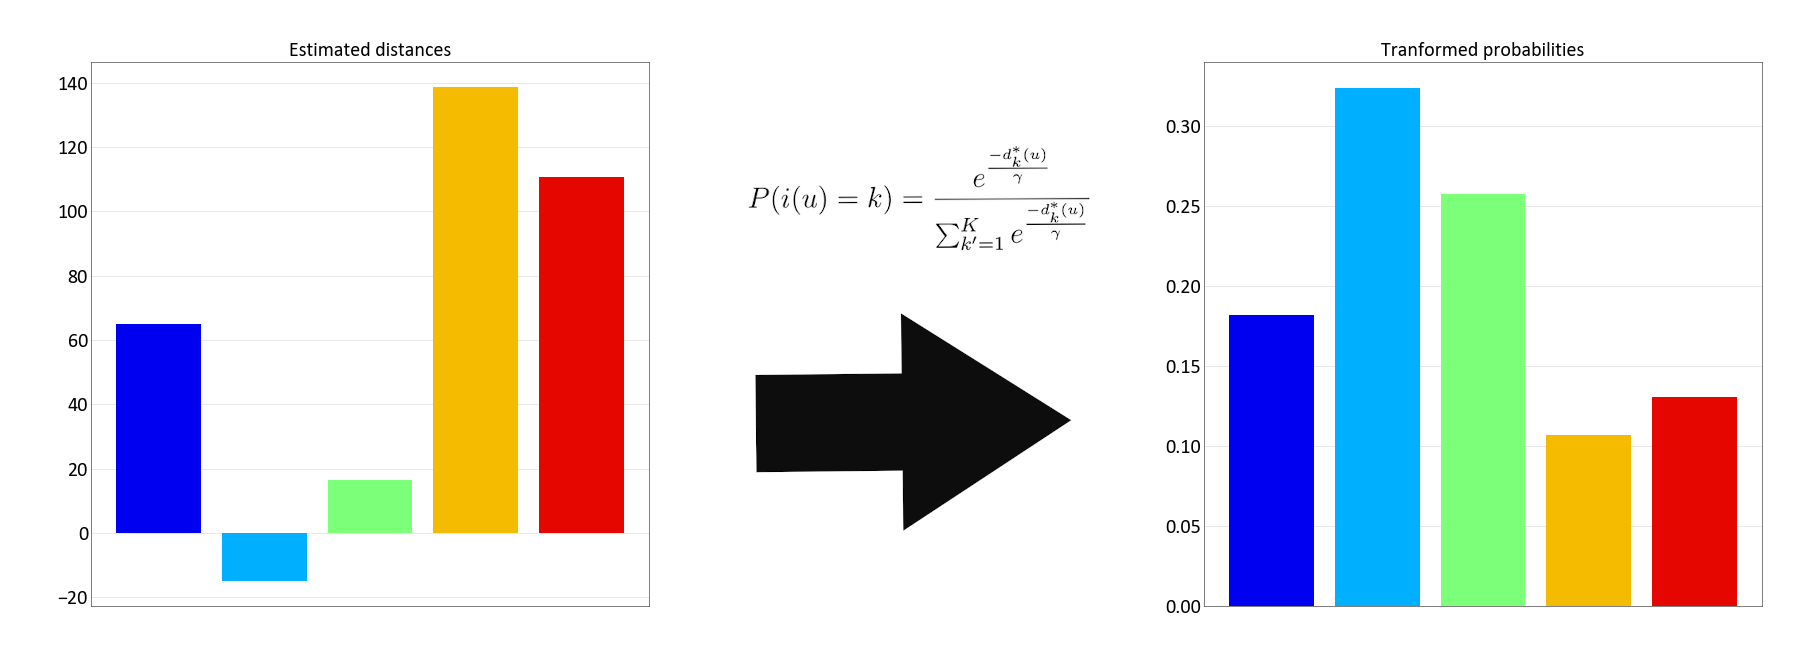
\includegraphics[width=0.7\textwidth]{capitulo_2/imagens/dis_to_probs.png}
\end{figure}

A \autoref{omega_ent} mostra a relação entre $\omega$ e a entropia de Shannon \cite{shannon1948mathematical} calculada pela \autoref{shannon_entr} para o bloco da \autoref{softmax_grafico}. $P(X_k)$ é a probabilidade para a categoria k. Para pequenos valores de $\omega$, uma das categorias será transformada em uma probabilidade muito alta, enquanto as outras serão transformadas em probabilidades muito baixas, nesse caso a entropia é mínima. À medida que o parâmetro $\omega$ aumenta, a diferença entre as probabilidades torna-se menos pronunciada até que a probabilidade para todas as categorias seja igual, caso em que a entropia é maximizada.

\begin{equation}
	H(X)=-\sum_{k=1}^{K}P(X_{k})log(P(X_{k}))
    \label{shannon_entr}
\end{equation}

\begin{figure}[H]
\caption{\label{omega_ent} Relação entre o parâmetro $\omega$ e a entropia de Shannon.}
	\centering
		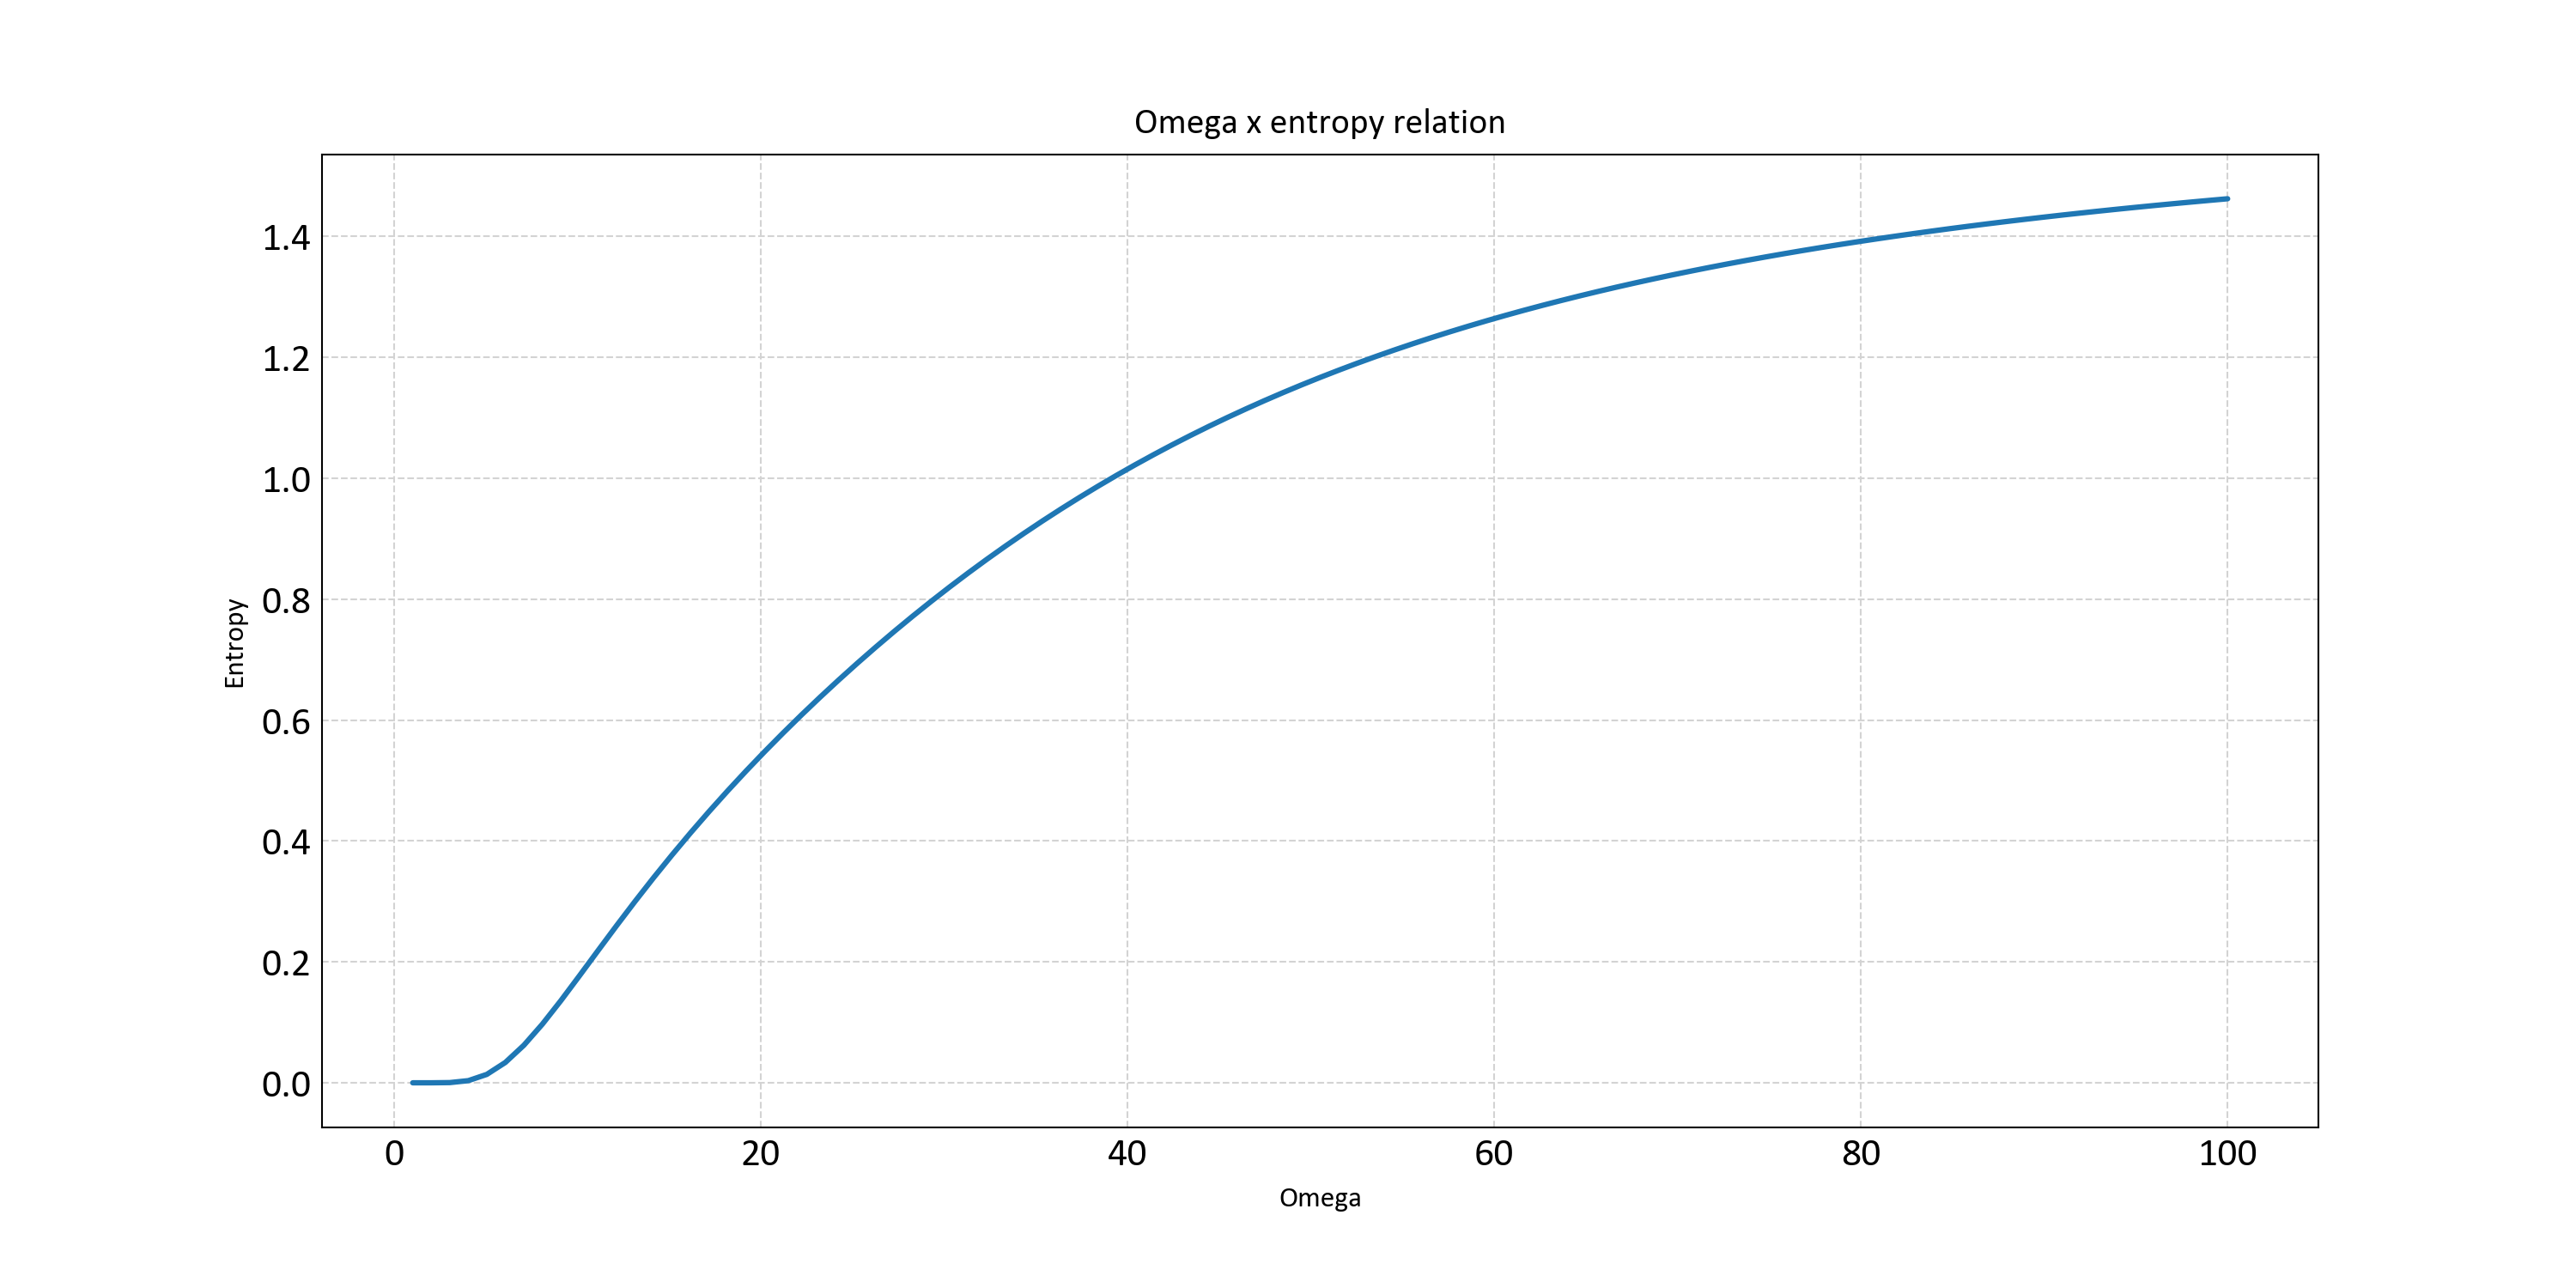
\includegraphics[width=0.8\textwidth]{capitulo_2/imagens/omega_entropy.png}
\end{figure}

A \autoref{jura_prob} mostra, à esquerda, as probabilidades para a categoria Quaternary obtidas transformando as distâncias assinaladas com o valor de $\omega$ igual a 10. Para esse valor do parâmetro há muitas regiões com probabilidade zero ou um de ocorrência e algumas regiões de transição próximas aos contatos. Ao centro, as probabilidades calculadas a partir das distâncias para $\omega$ igual a 100, nesse caso, há uma menor diferença entre as probabilidades. Por fim, à direita, as probabilidades foram calculadas usando como parâmetro $\omega$ o maior módulo entre as distâncias estimadas.

\begin{figure}[H]
    \centering
    \caption{Distâncias transformadas em probabilidades para a categoria Quaternary usando valores diferentes para $\omega$.} \label{jura_prob}
     \subfloat[][$\omega = 10$.]{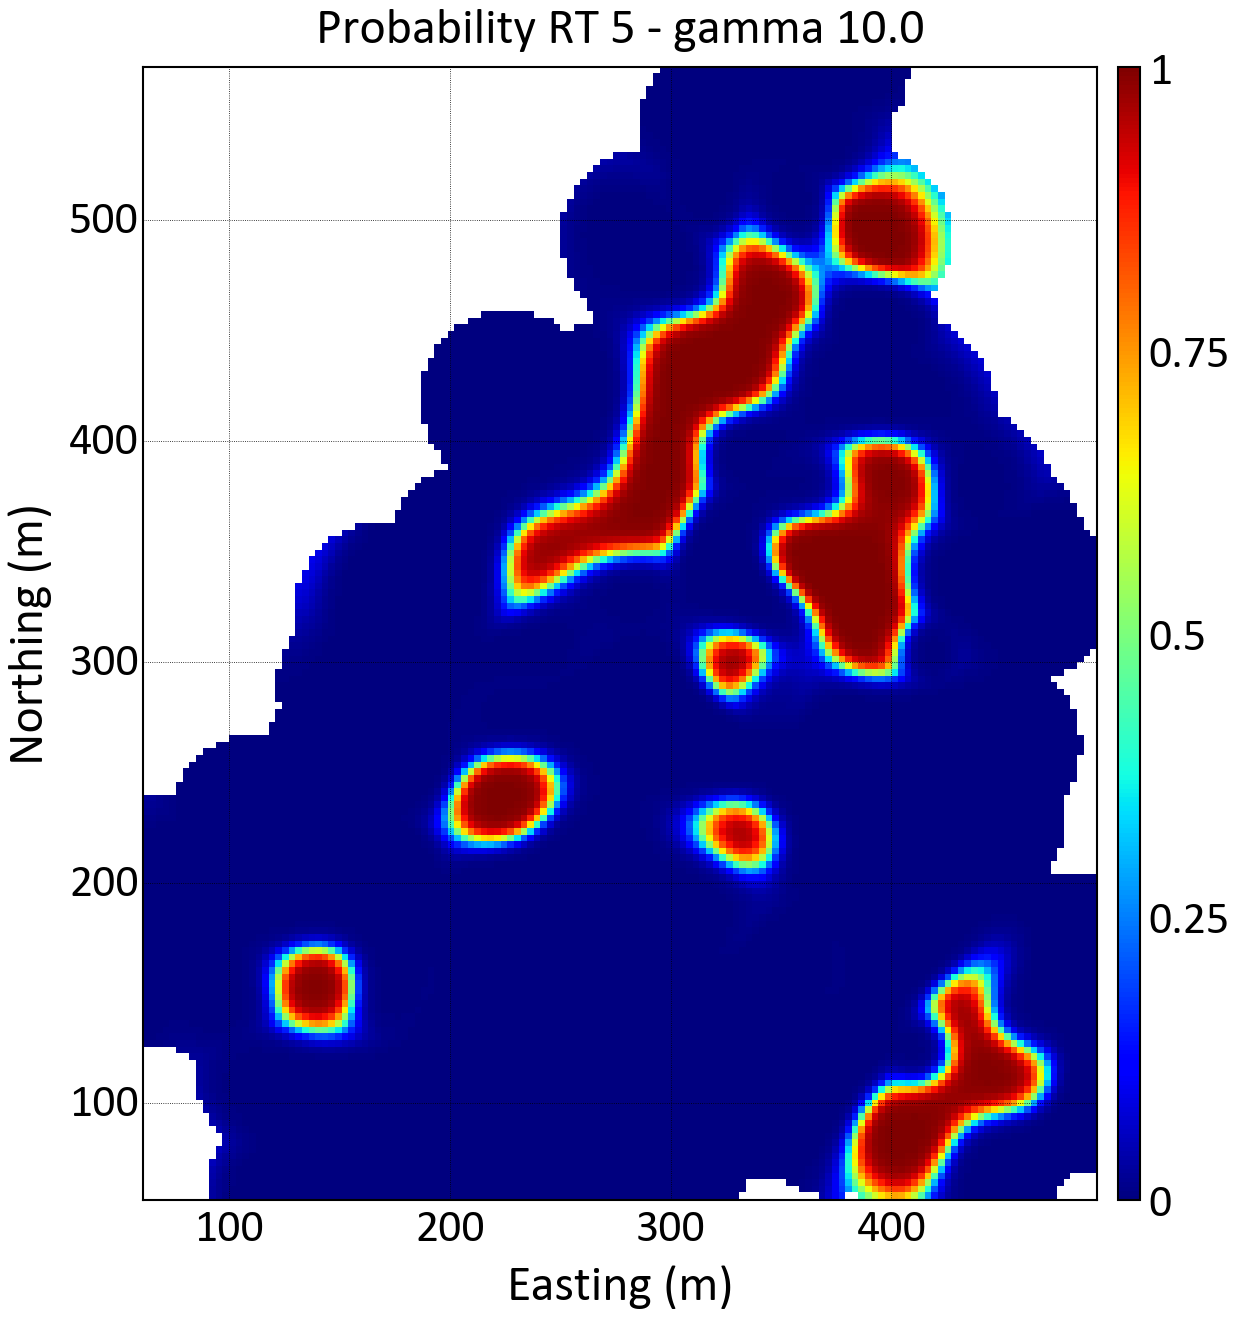
\includegraphics[width=.3\textwidth]{capitulo_2/imagens/probs_100.png}\label{<figure1>}}
     \hspace{1em}
     \subfloat[][$\omega = 100$]{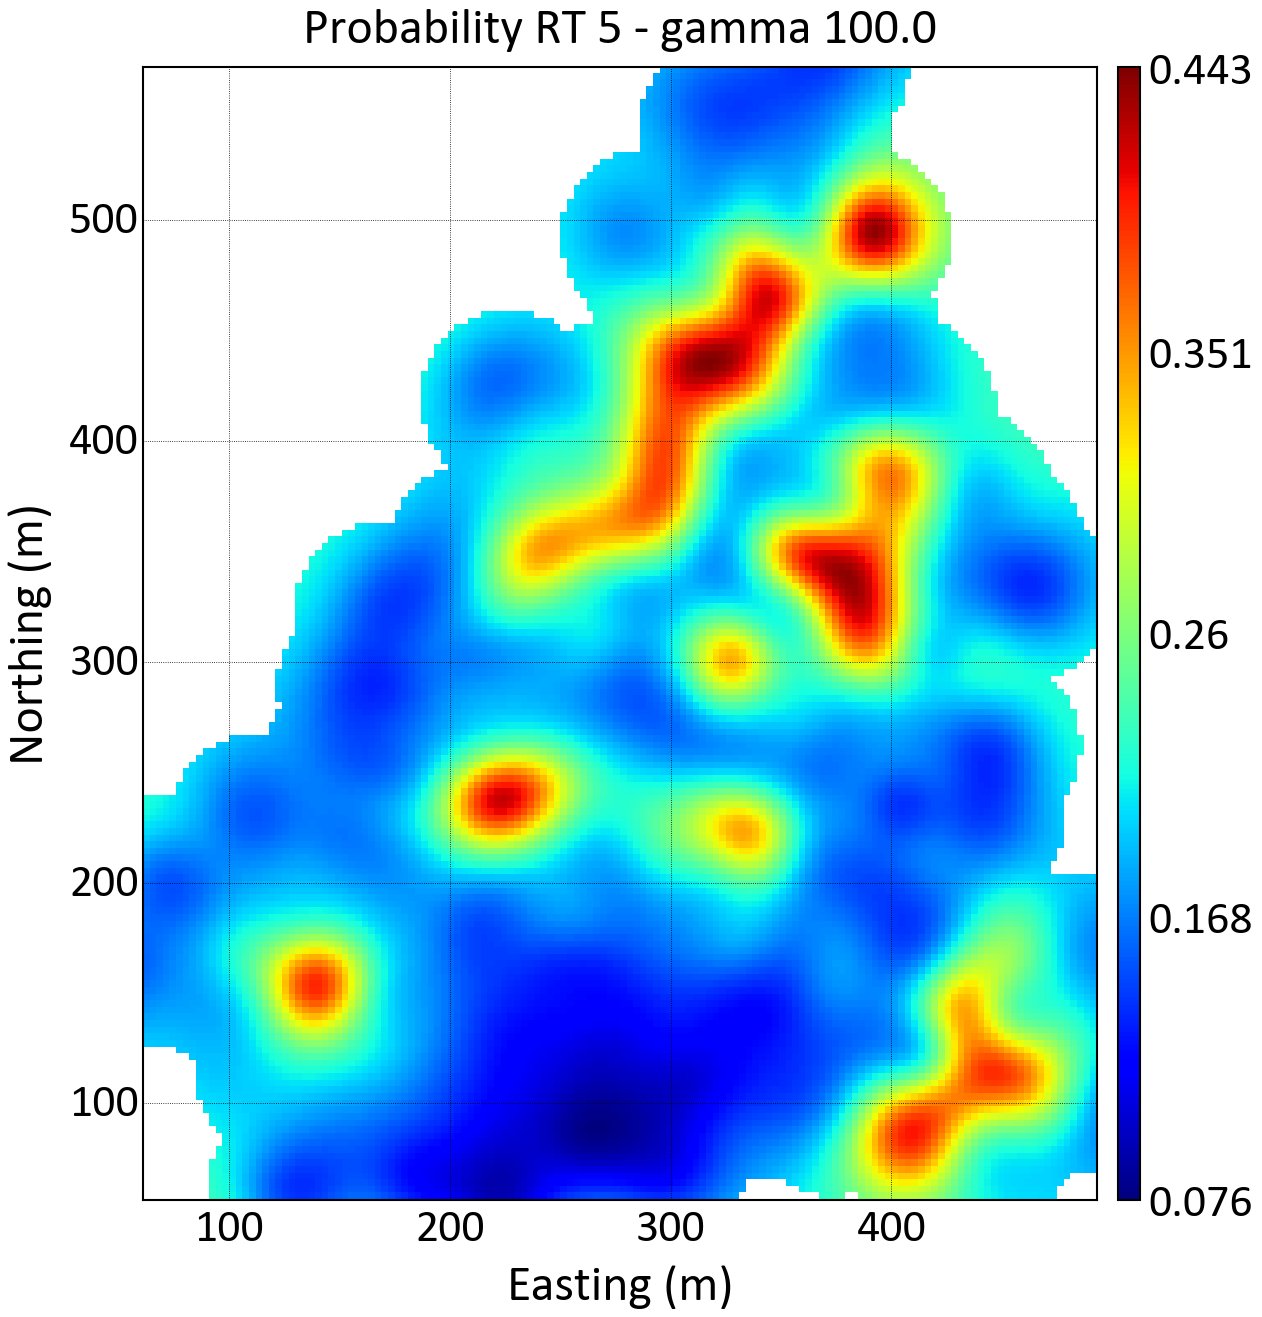
\includegraphics[width=.3\textwidth]{capitulo_2/imagens/probs_1000.png}\label{<figure2>}}
     \hspace{1em}
     \subfloat[][$\omega = $ maior módulo entre as distâncias estimadas.]{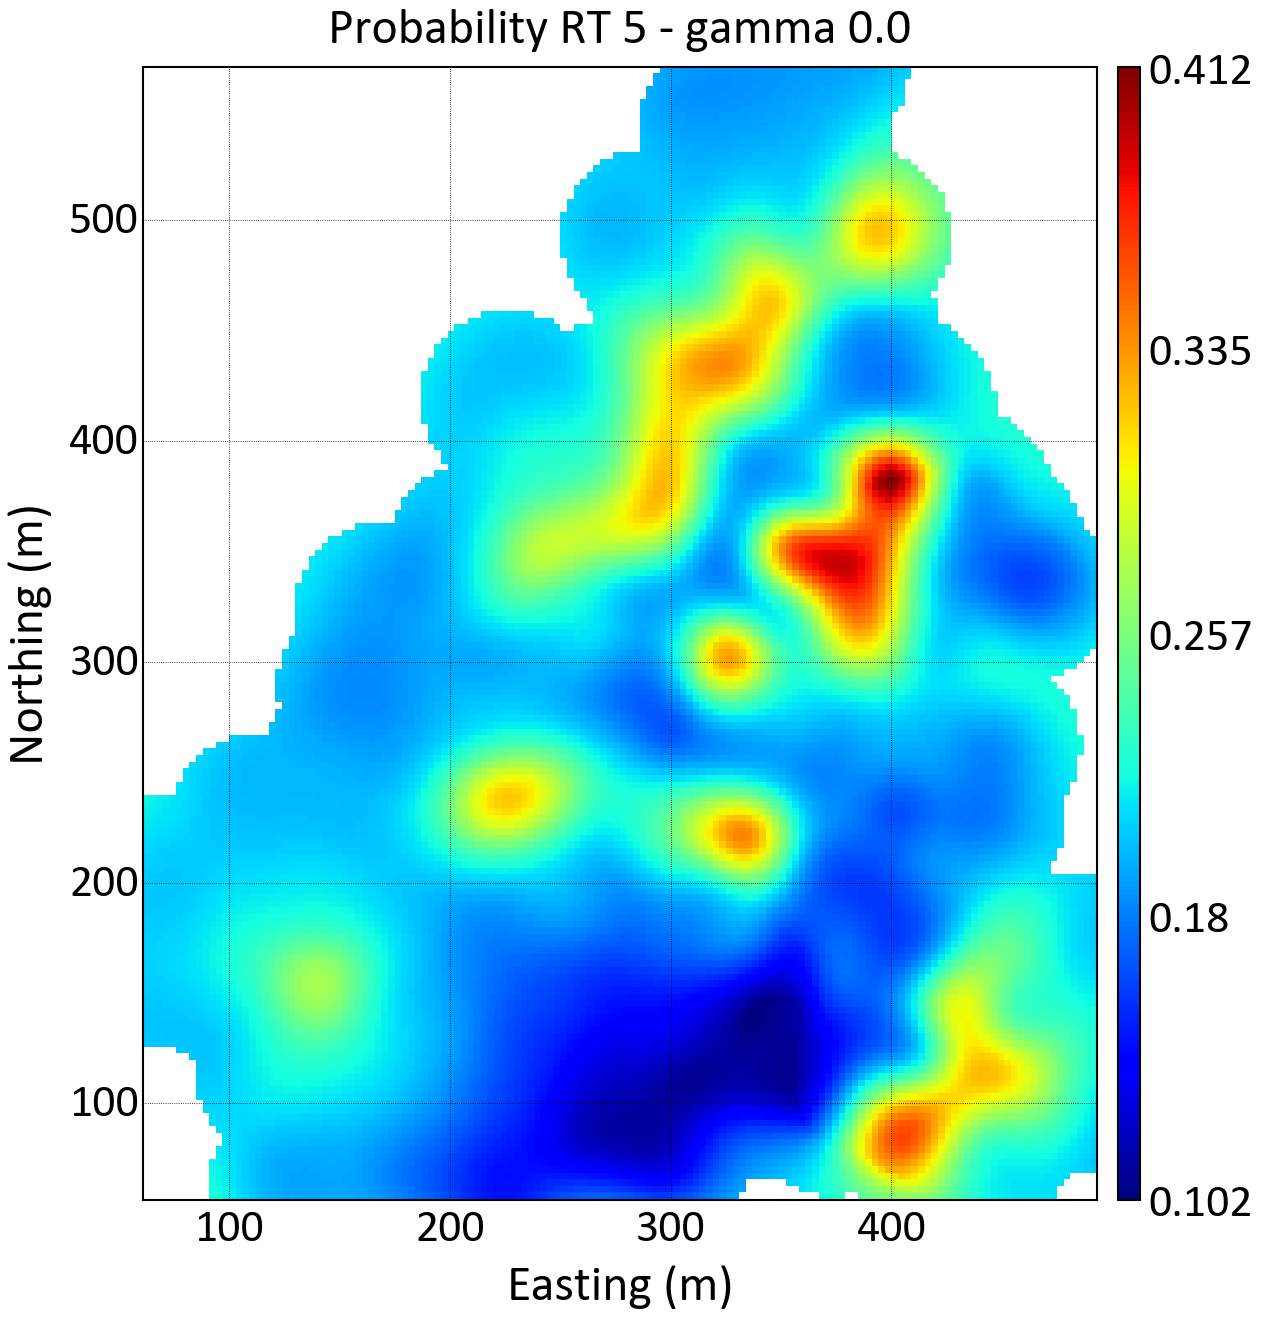
\includegraphics[width=.3\textwidth]{capitulo_2/imagens/probs_00.png}\label{<figure3>}}
\end{figure}

Apesar do método ser simples e direto, suportar múltiplas categorias simultaneamente, seu resultado não pode ser utilizado em etapas subsequentes do processo de  avaliação de recursos, por não gerar múltiplas realizações do modelo geológico.

\subsubsubsection{\textit{Boundsim}}

Uma outra metodologia proposta por \citeonline{mclennanstationarity, mclennan2006boundsim} consiste em realizar um \textit{bootstrap} espacial \cite{deutsh_spatial_bootstrap} da média da distância assinalada calculada para uma dada categoria. O procedimento de \textit{bootstrap} é amplamente utilizado para quantificar incerteza em parâmetros estatísticos. As duas mais importantes suposições são: os dados são representativos e os dados são independentes. Por esse motivo, a técnica de amostragem deve ser modificada para variáveis que apresentam continuidade espacial.

Diferentes valores para a média são tomados do histograma da média da distância assinalada, gerado pelo \textit{bootstrap} espacial. Esses valores podem ser correspondentes ao p10, p50 e p90 por exemplo. Então, as distâncias assinaladas são interpolados para os nós do \textit{grid} por krigagem simples, que tem como hipótese a estacionariedade da média por todo o domínio. A média estacionária para a krigagem simples são os valores tomados do histograma.

O último passo consiste em extrair a isosuperfície zero dos modelos implícitos gerados por krigagem simples com os diferentes valores da média estacionária tomadas do histograma da média. Em tese, quanto maior o percentil menor o risco associado, o volume do sólido modelado expande ou contrai de acordo com o valor escolhido para a média estacionária.

A metodologia é simples e direta, porém, deve ser aplicada à uma categoria por vez, na presença de múltiplos domínios alguma abordagem hierárquica deve ser estabelecida. A sensibilidade da krigagem simples à média depende da configuração espacial das amostras, muitas vezes a diferença entre os volumes obtidos é irrelevante.

O produto final do método pode ser utilizado nas etapas subsequentes do processo de avaliação, todavia, o método não avalia incerteza de forma adequada. Os autores do estudo original aplicaram a metodologia apenas em bancos de dados sintéticos e de geometria regular.

\subsubsubsection{Condicionamento das amostras}\label{chap:cond_amo}

\citeonline{mclennanstationarity} também propôs uma metodologia baseada na parametrização das amostras e posterior estimativas. Os pesos de krigagem e da interpolação pelo inverso da distância dependem do arranjo geométrico das amostras mas não dos valores das amostras. A proposta é alterar os pesos dados às amostras a partir de um fator de condicionamento $f^{DC}_i(u)$, como apresentado na \autoref{estimador_cond}

\begin{equation}
\label{estimador_cond}
d^*(u)=\sum_{i=1}^{n} f^{DC}_i(u) \lambda_i(u) d(u_i)
\end{equation}

Onde $d^*(u)$ é a distância interpolada no local não amostrado $u$, $d(u_i)$ são as distâncias assinaladas calculadas para as amostras, $\lambda_i(u)$ são os pesos dados pela krigagem ou inverso da distância e $f^{DC}_i(u)$ são os fatores de condicionamento que dependem do valor numérico das amostras. A krigagem ou inverso da distância clássicos apresentam um fator de condicionamento igual a um para todas as amostras.

Limites pessimistas ou otimistas podem ser gerados a partir das parametrizações mostradas na \autoref{param}. A reta de inclinação negativa da Figura \autoref{paramlinear} dá cada vez mais peso para amostras de distância mais negativas, e cada vez menos peso para amostras mais positivas produzindo uma isosuperfície zero otimista. O domínio tem um volume maior em relação ao caso base onde $f^{DC}_i(u)$ é igual a um para todas as amostras independente do seu valor. O contrário acontece para a reta com inclinação positiva.

A magnitude da diferença entre os limites otimistas e pessimistas é dada pelo parâmetro fator mínimo, ou \textit{fmin}, escolhido pelo usuário. Um f mínimo igual a um, gera um fator igual a um para todas as amostas (estimativa clássica). Quanto maior o fator, maior a inclinação da reta, e consequentemente, maior a diferença entre os cenários. O valor de f mínimo pode ser diferente para os cenários otimista e pessimista.

A magnitude da diferença pode ser acentuada usando uma função quadrática (Figura \autoref{paramquadrat}) ao invés de uma linear.

\begin{figure}[H]
    \centering
    \caption{Parametrização das amostras.} \label{param}
     \subfloat[][Linear.]{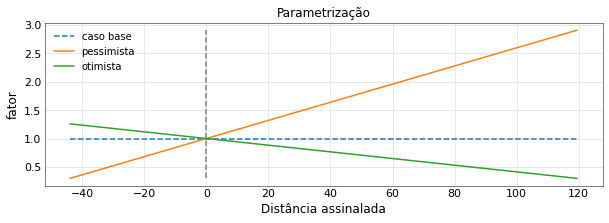
\includegraphics[width=.8\textwidth]{capitulo_2/imagens/linear_kfp.png}\label{paramlinear}} \\
     \subfloat[][Quadrática.]{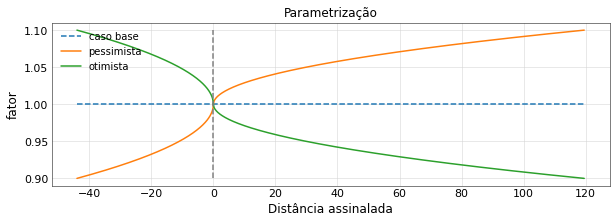
\includegraphics[width=.8\textwidth]{capitulo_2/imagens/quadratic_kfp.png}\label{paramquadrat}}
\end{figure}

\citeonline{mclennanstationarity} sugere o uso da interpolação pelo inverso da distância ao invés da krigagem porque os pesos negativos, que podem ser produzidos pela krigagem, interferem com o fator de parametrização.

\subsubsubsection{Simulação direta das distâncias assinaladas}\label{sim_direta}

\citeonline{caceres2011stochastic} e \citeonline{radtke_dissertacao} propuseram que as distâncias assinaladas sejam simuladas de forma direta: a partir de um modelo geológico implícito multi categórico, como o mostrado na \autoref{multicat_jura}, um coeficiente U de incerteza deve ser calculado de acordo com \autoref{u_eq}:

\begin{equation}\label{u_eq}
    U(u)=\frac{max\{D_{min}\}-min\{d^*_k(u)\}^K_{k=1}}{max\{D_{min}\}-min\{D_{min}\}}
\end{equation}

Onde:

\begin{equation}
    D_{min}=\{min\{d^*_k(u_1)\},...,\{min\{d^*_k(u_n)\}^K_{k=1}\}
\end{equation}

E $d^*_k(u)$ é a distância estimada no local u para a categoria k.

Os valores de U variam entre 0 e 1, um \textit{cutoff} em U determina a extensão da zona de incerteza ao redor dos contatos: quanto mais próximo de 1, mais estreita a zona. As distâncias assinaladas devem ser simuladas no interior da zona de incerteza e a categoria correspondente ao menor valor simulado é retida em cada bloco para cada realização. Os blocos simulados são concatenados com os blocos estáticos, atribuídos pela interpolação.

O método é baseado em múltiplas realizações do modelo geológico, então, seu produto final pode ser usado nas etapas posteriores do processo de avaliação. Entretanto, a metodologia tem muitos passos \cite{radtke_dissertacao}

\begin{enumerate}[label=\roman*]
\item Cálculo das distâncias assinaladas para todas as amostras e categorias;
\item Variografia das distâncias no espaço original para todas as categorias;
\item Interpolação das distâncias;
\item criação do modelo com base na menor distância interpolada;
\item Criação da zona de incerteza;
\item Transformação Gaussiana das distâncias;
\item Variografia das distâncias no espaço gaussiano para todas as categorias;
\item Geração de múltiplos modelos baseados na menor distância simulada;
\item Validação e pós processamento das realizações.
\end{enumerate}

Além disso, a simulação é muito sensível aos parâmetros, o que muitas vezes, gera modelos com excessivo ruído, que não são geologicamente realistas, e não honram as amostras. O resultado final não justifica o número demasiado de passos e parâmetros. O coeficiente U não controla a magnitude da incerteza, apenas diminui o tempo das simulações, a magnitude da incerteza é controlada pelos parâmetros da simulação.

\subsubsubsection{Avaliação de incerteza usando imagens de treinamento para simulação multi-ponto geradas a partir dos dados}

\citeonline{silvaenhancedgeomodeling} propôs uma metodologia que integra modelagem geológica implícita com funções distâncias assinaladas e simulação geostatística multi ponto. A geostatística multi-ponto utiliza imagens de treinamento para extrair e reproduzir estruturas geológicas complexas. Geralmente, imagens de treinamento são baseadas em modelos conceituais do fenômeno geológico. Em seu trabalho, \citeonline{silvaenhancedgeomodeling} cria imagens de treinamento a partir de modelos geológicos implícitos determinísticos criados com funções distância assinaladas e modelos estocásticos criados por simulação sequencial dos indicadores. No trabalho, é introduzida uma metodologia  para integrar múltiplas imagens de treinamento, uma metodologia para calibrar a contribuição de cada imagem de treinamento e uma medida de entropia multi-ponto ao longo dos furos de sondagem.

\citeonline{silvaenhancedgeomodeling} concluiu que imagens de treinamento geradas a partir das amostras produzem modelos geológicos estocásticos, por MPS, melhores.

\subsubsubsection{Modelagem estocástica de estruturas curvilineares}

\citeonline{lillah2013stochastic} propuseram a modelagem de estruturas curvilineares e a avaliação de incerteza desses modelos usando funções distância assinaladas. A metodologia tradicional é modificada para considerar não estacionariedade na forma de anisotropia variável localmente (LVA), que é incorporada na krigagem e na simulação sequencial Gaussiana das distâncias assinaladas. O campo de anisotropia variável captura a direção local, na qual a unidade geológica é mais contínua; enquanto, a simulação das distâncias e posterior extração da isosuperfície avalia a incerteza volumétrica.

\subsubsubsection{Avaliando e visualizando a incerteza com movimento estocástico}

\citeonline{yang2019assessing} propuseram uma técnica para avaliar e visualizar a incerteza em modelos geológicos multi-categóricos a partir do movimento estocástico. As unidades litológicas são representadas como uma soma de um modelo implícito estocástico conceitual com uma função residual condicionada às amostras e às relações cronológicas das unidades litológicas. Duas técnicas de amostragem para criação do movimento estocástico são propostas. Uma delas baseada na simulação de Monte Carlo e a outra em cadeias de Markov.

A incerteza é visualizada a partir de um filme no qual a transição entre as realizações é suave.

\subsubsubsection{Simulação dos contatos}\label{boundsim}

A metodologia proposta por \citeonline{wilde2012kriging} consiste em gerar realizações dos contatos geológicos comparando distâncias modificadas interpoladas com simulações não condicionais.

É necessário definir, antes de qualquer coisa, uma zona de incerteza em torno dos contatos. Blocos localizados fora da zona são considerados como pertencentes a um determinado indicador, enquanto blocos dentro da zona terão sua incerteza avaliada. A zona de incerteza é obtida a partir de um parâmetro C que controla sua espessura.

A escolha do parâmetro C depende do nível de precisão requerido versus o tempo necessário para calibrar o parâmetro. Assim, o parâmetro pode ser determinado de diferentes maneiras: a determinação empírica é baseada em valores pré-determinados e/ou no conhecimento do fenômeno considerando a geometria da amostragem e a experiência do geomodelador \cite{kaperov}. A calibração parcial compara modelos interpolados com um modelo de referência. O valor de C é determinado a partir da interpretação de seções geológicas representativas e da opinião de especialistas. A calibração total é demorada e trabalhosa: são necessários vários modelos de referência para determinar o parâmetro C \cite{kaperov}. Para cada modelo de referência, um algoritmo de otimização é usado para calcular o parâmetro C, e para uma única iteração é necessário interpolar todos os modelos de referência com o mesmo parâmetro C. Para alcançar a calibração completa, várias iterações são necessárias usando valores diferentes para o parâmetro C, que demanda um grande esforço computacional e aumenta o tamanho e o número dos modelos de referência usados \cite{munroe2008full}.

A calibração também pode ser realizada por um método semelhante à metodologia de validação cruzada por \textit{jackknife} \cite{wilde2012kriging}, utilizando apenas os dados para calibrar o parâmetro C com baixa demanda computacional e alta automatização.

O primeiro passo na calibração de C por \textit{jackknife} é remover um subconjunto dos dados. Isso pode ser feito escolhendo aleatoriamente os furos de sondagem a serem excluídos. Um estudo de calibração adequado envolve a geração de vários conjuntos, com diferentes proporções (50\% a 10\%) e diferentes configurações de dados removidos \cite{manchuck}. Os valores da função distância são então calculados para os dados restantes com um valor inicial para C igual a zero. Essas amostras da função distância assinaladas são usadas para condicionar a estimativa da função distância em cada um dos locais de dados removidos. Existem quatro resultados possíveis  desta estimativa. A localização pode ser: corretamente estimada como fora do domínio, corretamente estimada como dentro do domínio, incorretamente estimada como fora do domínio e incorretamente estimada como dentro do domínio. O principal interesse está no número de dados que caem do lado errado da fronteira, ou seja, o número de vezes que a estimativa é positiva, mas os dados são codificados como dentro do domínio e o número de vezes que a estimativa é negativa, mas o os dados são codificados como fora do domínio. O número de vezes que um dado cai do lado errado do limite para C igual a zero é o caso base.

O valor de C é então aumentado e os valores da função distância das amostras não removidas são modificados de acordo com a \autoref{C_dist}. Essa função distância modificada é estimada nos locais das amostras removidas. O limite agora é considerado como estando entre -C e C. Os dados caem do lado errado do limite quando um local estimado é codificado como interno, mas tem uma estimativa para a função distância modificada maior que C ou um local estimado é codificado como externo, mas tem uma estimativa da função distância modificada menor que -C. O número de dados que caem do lado errado do limite diminui à medida que C aumenta. C é aumentado até que o número de dados que caem no lado errado do limite seja aceitável. O valor C onde isso ocorre é o valor C calibrado que quantifica a incerteza do limite.

\begin{equation}
	d_k(u_\alpha)=\begin{cases}
	-\parallel u_\alpha-u_\beta\parallel - C,\:\textrm{se $u_\alpha$ pertence ao domínio}\\
	+\parallel u_\alpha-u_\beta\parallel + C,\:\textrm{se $u_\alpha$ não pertence ao domínio}\end{cases}
    \label{C_dist}
\end{equation}

A \autoref{c_uncert} mostra, para um esquema sintético em duas dimensões, em branco a zona considerada fora domínio, em preto dentro do domínio e em cinza a zona de contato para diferentes valores de C. À medida que C aumenta, o número de classificações errôneas diminui já que qualquer ponto estimado na zona cinza não é uma classificação errônea. Os sinais (+ e -) representam as amostras e sua distância assinalada calculada.

\begin{figure}[H]
	\caption{\label{c_uncert}Calibração do parâmetro C para um esquema em duas dimensões.}
	\centering
		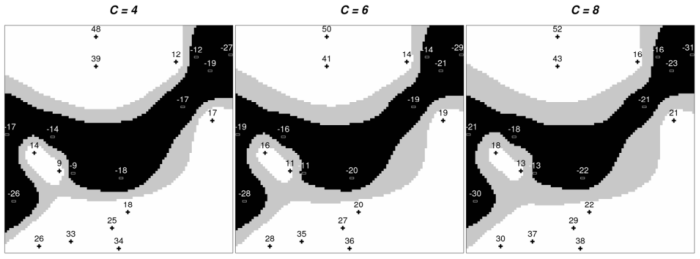
\includegraphics[width=0.8\textwidth]{capitulo_2/imagens/c_uncert.png}
	\legend{Fonte: \citeonline{wilde2012kriging}}
\end{figure}

Uma curva como a da \autoref{c_calib_grafico} é construída. São escolhidos N valores para C entre zero e um valor definido pelo usuário (linhas tracejadas em verde). Para cada um desses valores de C, são removidos X\% dos furos (ou amostras em duas dimensões) Z vezes (estrelas azuis). É indicado que a classificação errônea seja calculada diversas vezes para que a calibração de C seja robusta \cite{wilde2012kriging}. O índice de classificação errônea é registrado no eixo Y do gráfico (estrelas azuis) e o valor de C no eixo X (linhas tracejadas em verde). Então traça-se a classificação errônea média (curva em preto).

\begin{figure}[H]
	\caption{\label{c_calib_grafico}Figura esquemática da curva de calibração.}
	\centering
		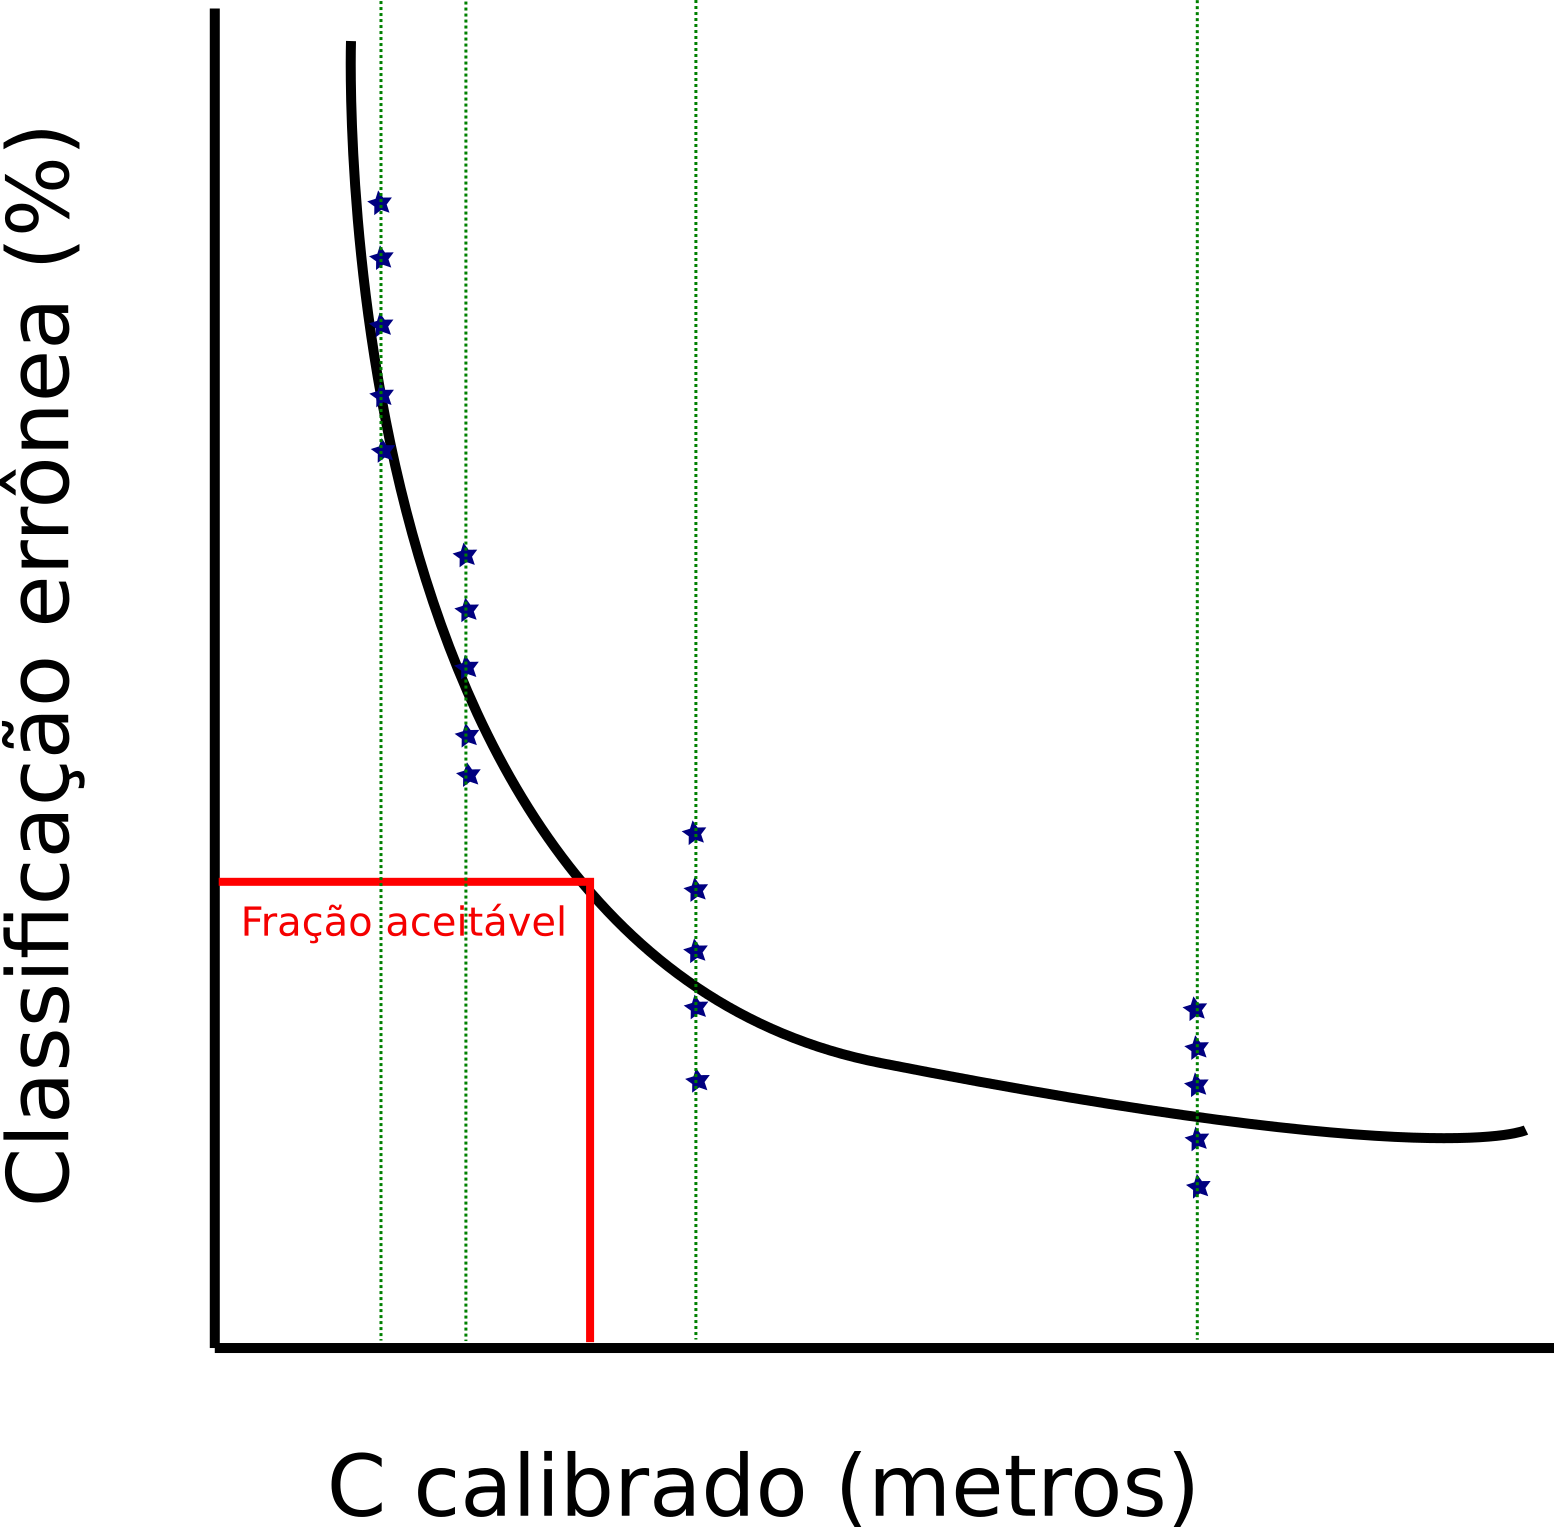
\includegraphics[width=0.4\textwidth]{capitulo_2/imagens/calibration.png}
\end{figure}

\citeonline{manchuck_deutsch_Geometric} sugerem 2,5\% de classificação errônea um nível aceitável para depósitos tabulares, \cite{martin2017implicitmodeling} definiram como 3.9\% para um dos domínios de um depósito de cobre. Uma outra forma de escolha é o método do cotovelo, o valor tomado deve ser o ponto de inflexão da curva de calibração \cite{martin2017implicitmodeling}. C depende do tipo de depósito e da configuração geométrica das amostras. Para depósitos com menor variabilidade, como os de bauxita por exemplo, C deve ser pequeno. Já para depósitos com maior variação, como os de ouro, o valor de C deve ser maior. Para amostragens densas o valor de C deve ser menor em relação à amostragens esparsas. C não deve ser maior do que a malha de sondagem.

Após o valor de C ser selecionado, as distâncias assinaladas calculadas para cada amostra devem ser modificadas a partir da equação \autoref{C_dist}. As distâncias modificadas devem então ser interpoladas, utilizando o mesmo variograma das distâncias originais, para todos os nós do \textit{grid}, e a truncagem das distâncias modificadas estimadas entre -C e +C define a zona de incerteza.

Valores para a função distância são simulados uniformemente entre -C e +C. Para isso, é necessário realizar uma simulação Gaussiana não condicional. Um dos algoritmos comumente usados é a simulação sequencial Gaussiana (\autoref{algo:usgs}). A simulação sequencial Gaussiana não condicional gera valores Gaussianos (contínuos) que reproduzem o variograma informado. O variograma utilizado na simulação não condicional pode ser o mesmo das distâncias assinaladas. O alcance do variograma determina a natureza do contato entre os domínios, menores alcances geram contatos mais rugosos enquanto maiores alcances, contatos suaves. O efeito pepita controla a inter conectividade entre o domínio.

\begin{algorithm}
\SetAlgoLined
    1. Defina um caminho aleatório através dos nós do \textit{grid}\;
    \For{cada nó}{
    1. Busque no espaço por nós previamente simulados\;
    \eIf{número de nós previamente simulados != 0}{
    1. Construa e resolva o sistema de krigagem\;
    2. Amostre a distribuição condicional construída a partir da média e da variância\;
    }{
    1. Amostre a partir de uma distribuição Gaussiana padrão\;
    }
    2. Atribua o valor amostrado ao nó do modelo e inclua o nó simulado no conjunto de dados simulado anteriormente\;
    }
 \caption{Simulação sequencial Gaussiana não condicional}\label{algo:usgs}
\end{algorithm}

Para que os valores simulados se distribuam de forma uniforme entre –C e +C, o valor Gaussiano, deve ser transformado pela relação:

\begin{equation}
\label{sim_trans}
    df'(u)=2*C*G^-1(y'(u))-C
\end{equation}

Onde: $df'(u)$ é o valor da função distância simulada, $y'(u)$ o valor normal padrão da simulação não condicional, e $G^-1$ representa a determinação do valor da distribuição acumulada padrão normal correspondente a $y'(u)$. Para garantir que os valores pertençam a região estabelecida os valores são multiplicados por 2C e subtraídos de C.

A \autoref{sim_zona_c} mostra duas realizações da simulação das distâncias para uma zona de incerteza igual a 5 metros para o esquema em duas dimensões da \autoref{c_uncert}.

\begin{figure}[H]
	\caption{\label{sim_zona_c}Simulação das distâncias dentro da zona de incerteza para um esquema em duas dimensões.}
	\centering
		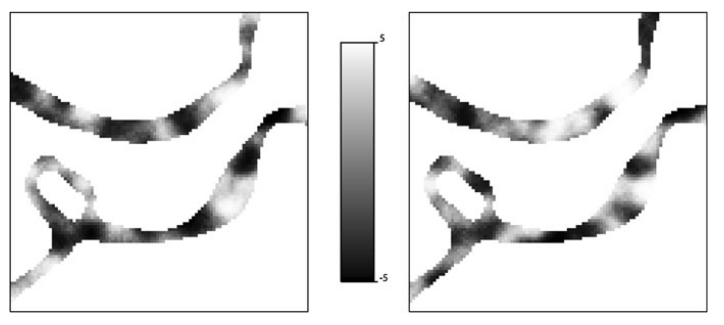
\includegraphics[width=0.8\textwidth]{capitulo_2/imagens/sim_zona_c.png}
	\legend{Fonte: \citeonline{wilde2012kriging}}
\end{figure}

Os contatos podem agora ser simulados no interior da zona de incerteza. Caso o valor interpolado $df^{*}(u)$ seja menor que o valor simulado $df'(u)$ para a função distância, o local é considerado pertencente ao domínio (indicador 1), caso o valor interpolado seja maior que o simulado, o local é considerado externo ao domínio (indicador 0), como evidenciado pela \autoref{comp_class}. Nos locais onde a interpolação apresenta o mesmo valor da simulação, são estabelecidos os contatos dos domínios como esquematizado na \autoref{conceptual}.

\begin{equation}
\label{comp_class}
	i`(u)=\begin{cases}
	indicador \: 1, \: se \: df'(u) > df^{*}(u)\\
	indicador \: 0, \: se \: df'(u) < df^{*}(u)\end{cases}
\end{equation}

\begin{figure}[H]
	\caption{\label{conceptual}Esquema mostrando como os contatos são simulados dentro da zona de incerteza.}
	\centering
		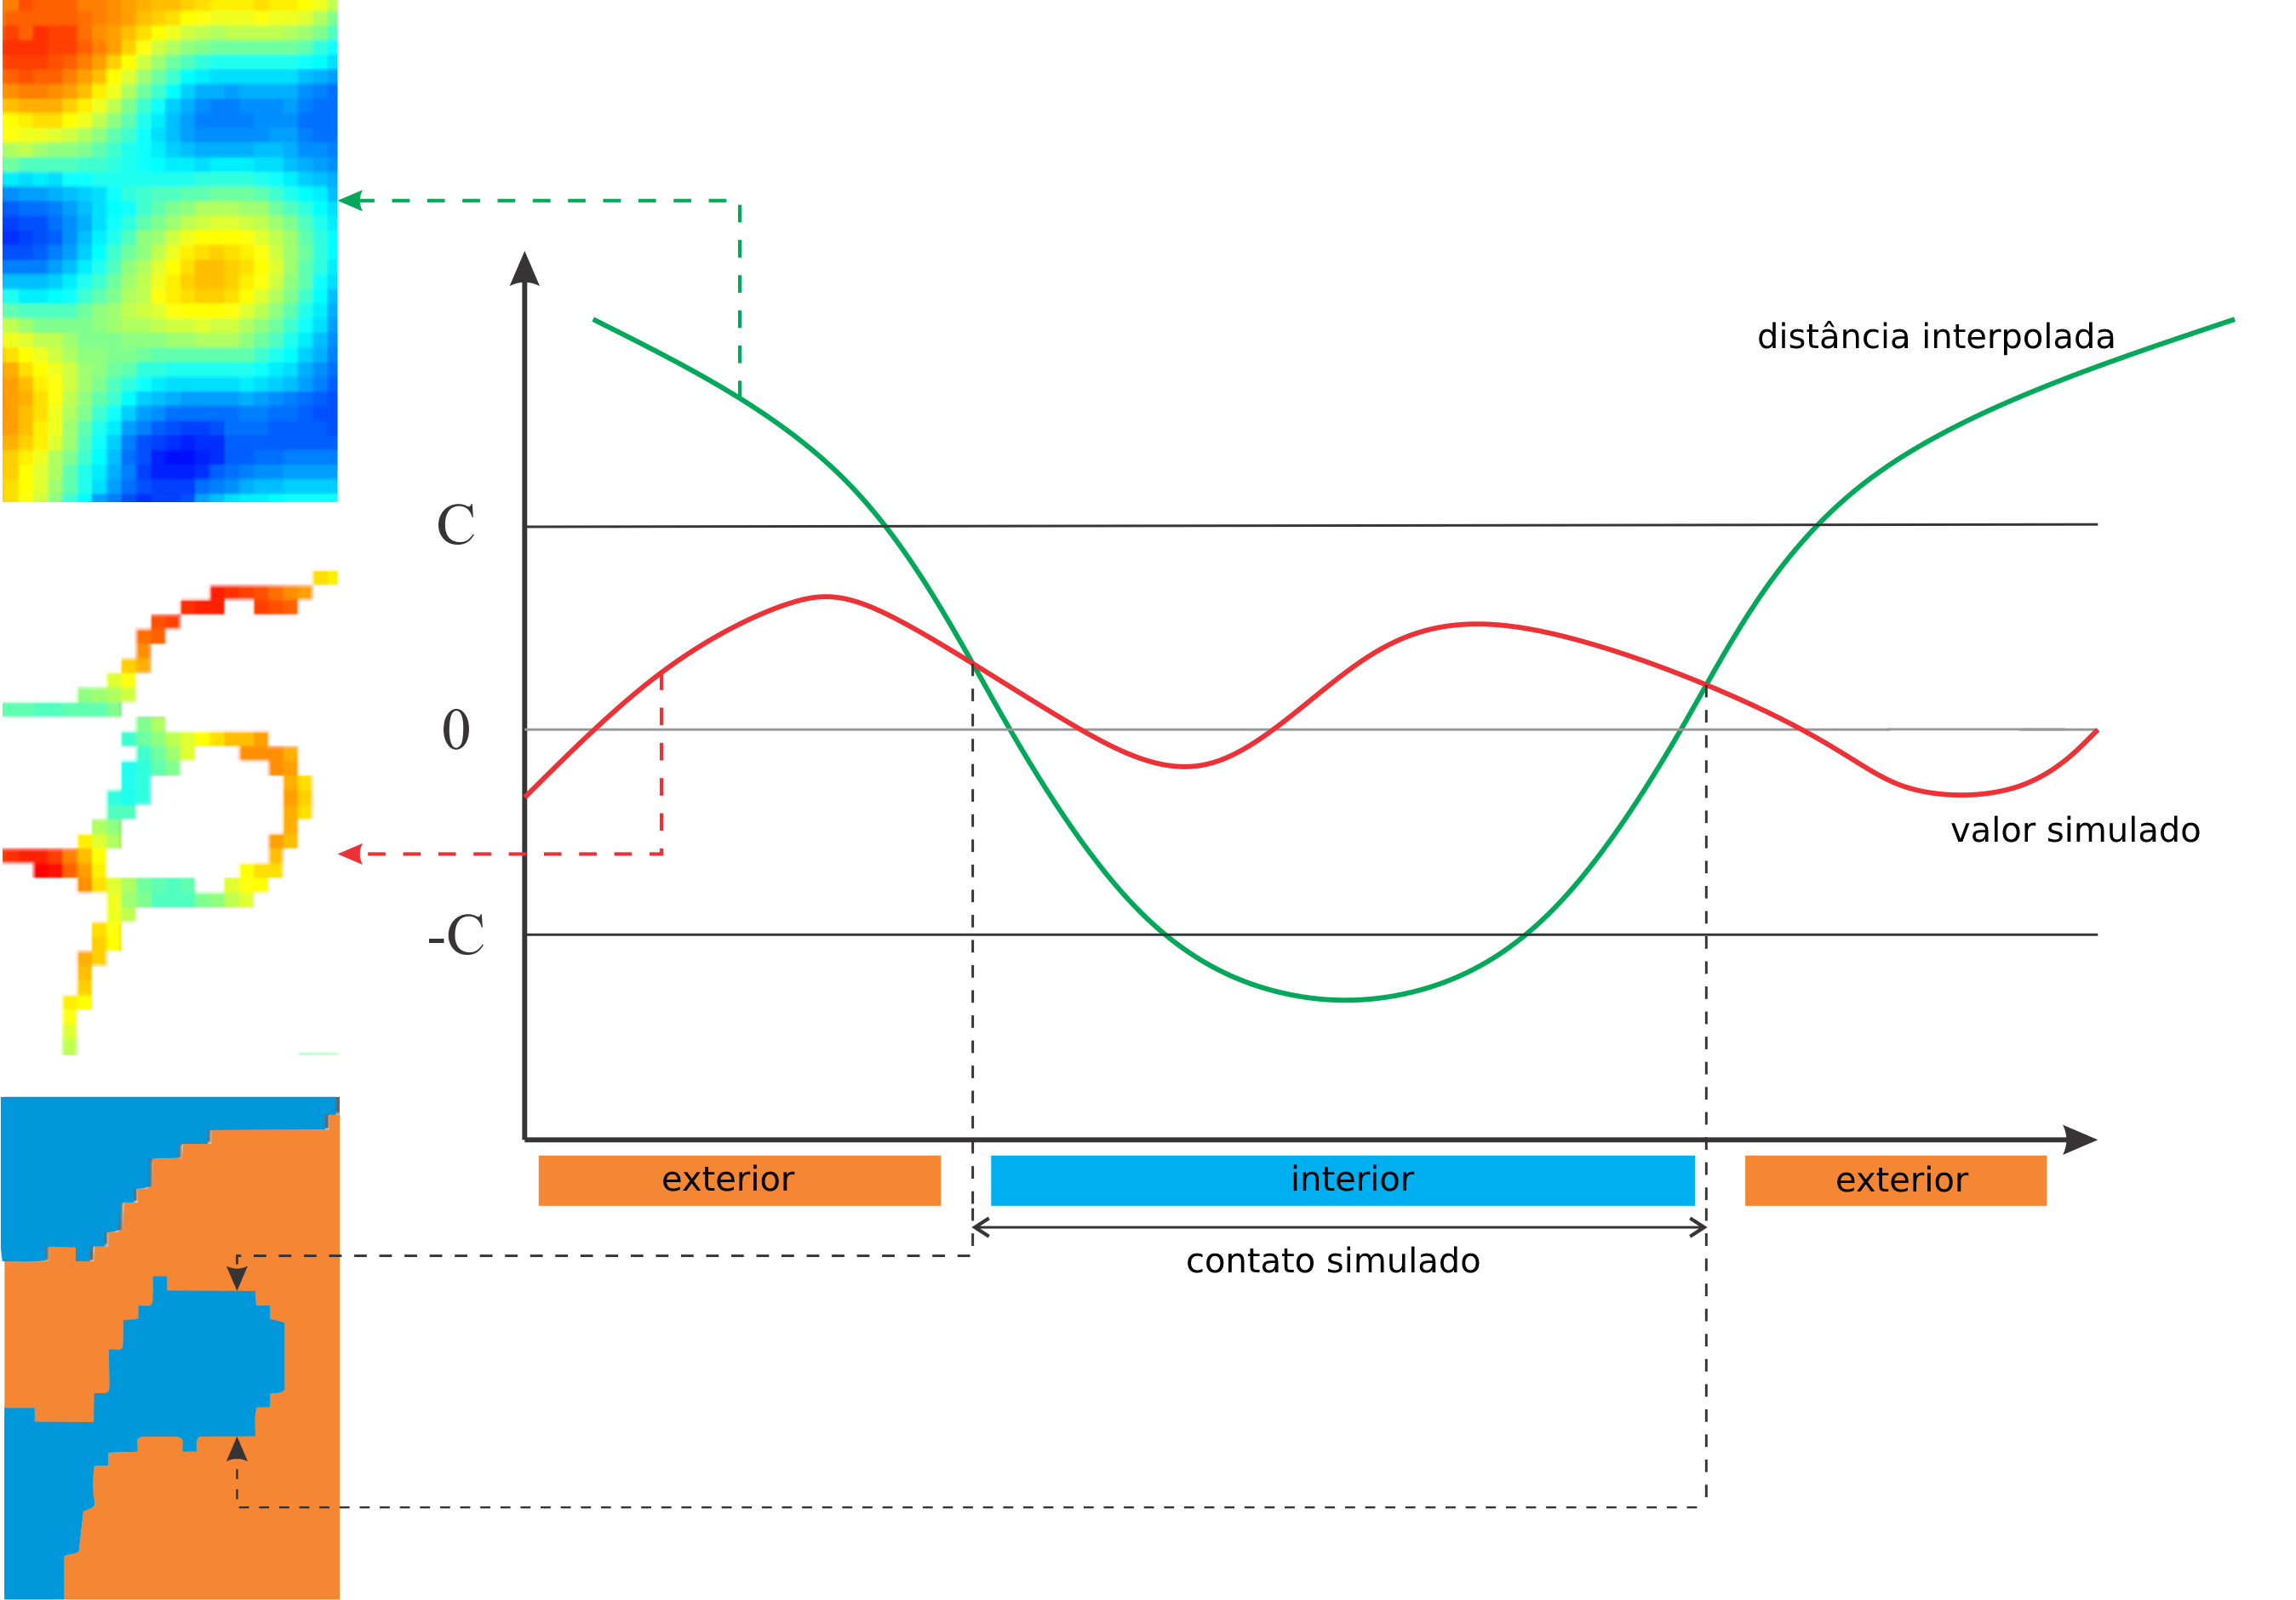
\includegraphics[width=\textwidth]{capitulo_2/imagens/conceptual.png}
		\legend{Modificado de \citeonline{amarante2021boundary}}
\end{figure}

A \autoref{final_result} mostra duas diferentes realizações da simulação dos contatos para o esquema em duas dimensões mostrado na \autoref{c_uncert}.

\begin{figure}[H]
	\caption{\label{final_result}Duas realizações da simulação dos contatos para um esquema em duas dimensões.}
	\centering
		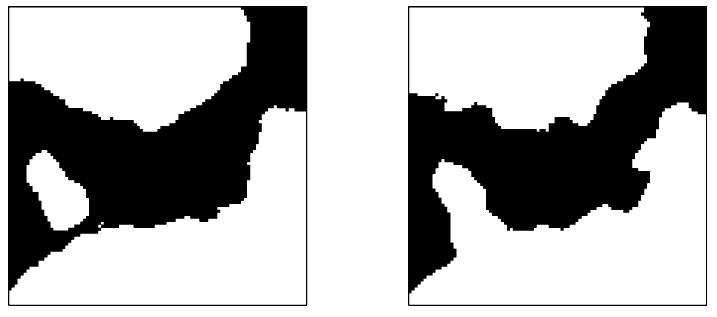
\includegraphics[width=0.8\textwidth]{capitulo_2/imagens/final result.png}
	\legend{Fonte: \citeonline{wilde2012kriging}}
\end{figure}

O método é rápido, já que é baseado em simulações não condicionais, gera modelos realista,s sem ruído e com fronteiras contínuas. Tanto a magnitude da incerteza, quanto a natureza da fronteira podem ser controlados. Entretanto, o método funciona apenas para uma categoria por vez e mesmo que simplificações tenham sido desenvolvidas, a calibração do parâmetro de incerteza ainda pode ser laboriosa e subjetiva.

\chapter{Metodologias propostas}\label{chap3}

Esse capítulo propõe três metodologias para avaliação de incerteza em modelos geológicos multi-categóricos usando funções distâncias assinaladas. Todos os métodos são acompanhados de uma prova de conceito no banco de dados \textit{Swiss Jura} e um estudo de caso. 

\section{Parametrização do suporte do \textit{kernel}}

Esse método é uma adaptação do condicionamento das amostras apresentado no \autoref{chap:cond_amo}, para que além de poder ser aplicado para múltiplos domínios, seja mais versátil. No método proposto por \citeonline{mclennanstationarity} o interpolador fica restrito ao inverso do quadrado já que outros interpoladores podem gerar pesos negativos que interferem na ponderação gerada pelo condicionamento das amostras.

A adaptação propõe, no lugar de modificar o peso dado às amostras, modificar o suporte dos \textit{kernels} usados na interpolação por funções de bases radiais multiplicando-os por um fator menor (pessimista) ou maior (otimista) que um. Para cada categoria do depósito mineral, os cenários otimistas, pessimista e caso base são gerados e combinados para criar múltiplos cenários para o modelo geológico multi-categórico.

Considere o exemplo em uma dimensão da \autoref{one_dim_ex}. A figura mostra quatro amostras, duas azuis que não pertencem ao domínio sendo modelado, e duas vermelhas que pertencem ao domínio sendo modelado. As amostras estão, da esquerda para a direita, nas posições 1, 10, 70 e 90.

\begin{figure}[H]
	\caption{\label{one_dim_ex} Amostras em posição 1, 10, 70 e 90. Amostras em azul não pertencem ao domínio enquanto amostras vermelhas pertencem.}
	\centering
		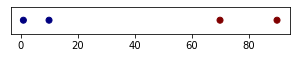
\includegraphics[width=0.4\textwidth]{capitulo_3/imagens/pointssd.png}
\end{figure}

A \autoref{uni_rbf} mostra, no gráfico horizontal abaixo as amostras da \autoref{one_dim_ex} e no eixo y do gráfico o valor da função distância assinalada calculada para cada uma das quatro amostras. A Figura \autoref{at} uma função RBF com suporte igual a 25 centrada em cada uma das amostras. A Figura \autoref{dt} mostra, em preto, a superfície interpolada a partir da combinação das quatro RBFs após o cálculo dos pesos a partir do sistema de equações apresentado na \autoref{rbf_sist}. O limite do domínio é onde a distância assinalada interpolada é igual a zero.

\begin{figure}[H] 
    \centering
    \caption{Exemplo em uma dimensão no gráfico abaixo e distâncias assinaladas calculadas para cada uma das amostras no eixo y.} \label{uni_rbf}
     \subfloat[][Uma RBF com suporte igual a 25 e centrada em cada uma das amostas.]{\includegraphics[width=.45\textwidth]{capitulo_3/imagens/RBF_before_train.png}\label{at}}
     \hspace{1em}
     \subfloat[][Uma RBF com suporte igual a 25 e centrada em cada uma das amostas após o cálculo dos pesos e sua combinação linear em preto.]{\includegraphics[width=.45\textwidth]{capitulo_3/imagens/RBF_after_train.png}\label{dt}}
\end{figure}

O método proposto modifica o suporte de uma cada uma das RBFs centradas nas amostras de acordo com o valor da distância assinalada calculada para aquela amostras a partir das curvas de parametrização mostradas na \autoref{param}. Dessa forma, cada RBF terá um suporte diferente. O volume do sólido gerado pelo cenário otimista é maior do que o gerado pelo caso baso enquanto o volume do sólido gerado pelo caso pessimista é menor.

\begin{figure}[H] 
    \centering
    \caption{Parametrização das amostras.} \label{param}
     \subfloat[][Linear.]{\includegraphics[width=.8\textwidth]{capitulo_3/imagens/linear_kfp.png}\label{paramlinear}} \\
     \subfloat[][Quadrática.]{\includegraphics[width=.8\textwidth]{capitulo_3/imagens/quadratic_kfp.png}\label{paramquadrat}}
\end{figure}

A \autoref{dif_kernel} mostra as RBFs, que na \autoref{uni_rbf} tinham suporte igual a 25, com seus suportes modificados a partir das curvas de parametrização lineares mostradas na Figura \autoref{paramlinear}. Os pesos são então calculados para cada um dos casos e uma superfície interpolada pode ser gerada a partir da combinação linear das RBFs.

\begin{figure}[H] 
    \centering
    \caption{Exemplo em uma dimensão no gráfico abaixo e distâncias assinaladas calculadas para cada uma das amostras no eixo y.} \label{dif_kernel}
     \subfloat[][Caso otimista.]{\includegraphics[width=.45\textwidth]{capitulo_3/imagens/pessimistic_kernels.png}\label{<figure1>}}
     \hspace{1em}
     \subfloat[][Caso pessimista.]{\includegraphics[width=.45\textwidth]{capitulo_3/imagens/optmistic_kernels.png}\label{<figure2>}}
\end{figure}

A \autoref{one_dim_result} mostra, em preto, a superfície interpolada para o caso base, em vermelho, para o cenário pessimista e em azul para o cenário otimista. 
 
\begin{figure}[H]
	\caption{\label{one_dim_result} Caso base e cenários otimista e pessimista para o exemplo unidimensional proposto.}
	\centering
		\includegraphics[width=0.6\textwidth]{capitulo_3/imagens/all_kernels.png}
\end{figure}

A aplicação do método no banco de dados \textit{Swiss Jura} consiste em, calcular as distâncias assinaladas para cada uma das cinco categorias do banco de dados. Então os parâmetros para modificação do suporte devem ser escolhidos. Nesse caso, um modelo linear com valor de f mínimo igual a 0.95. A \autoref{quater_param} mostra as distâncias assinaladas para a categoria Quaternary interpoladas para o cenário pessimista, caso base e cenário otimista. Os mesmos cenários foram interpolados para as outras quatro categorias do banco de dados.

\begin{figure}[H] 
    \centering
    \caption{Distâncias assinaladas interpoladas para a categoria Quaternary do banco de dados \textit{Jura} para o caso base, e cenários pessimista e otimista.} \label{quater_param}
     \subfloat[][Caso pessimista.]{\includegraphics[width=.3\textwidth]{capitulo_3/imagens/pessimistic.png}\label{<figure1>}}
     \hspace{1em}
     \subfloat[][Caso base.]{\includegraphics[width=.3\textwidth]{capitulo_3/imagens/intermediate.png}\label{<figure2>}}
     \hspace{1em}
     \subfloat[][Caso otimista.]{\includegraphics[width=.3\textwidth]{capitulo_3/imagens/optimistic.png}\label{<figure3>}}
\end{figure}

Para cada categoria há três diferentes cenários que devem ser combinados para criar os modelos geológicos multi-categóricos. Em alguns casos, a combinação do cenário otimista de uma categoria com grande área ou grande volume com o cenário pessimista de uma categoria de pequena área ou volume pode fazer com nenhum bloco seja atribuído à menor categoria em alguns dos $3^K$ modelos. Onde K é o número de categorias do banco de dados.  

Para contornar esse problema os modelos devem passar por um teste de reprodução dos dados amostrais. O algoritmo checa se o bloco com o centroide mais próximo a cada amostra foi classificado com a mesma categoria daquela amostra. O usuário seleciona um nível mínimo de reprodução, nesse caso 0.9. Desse modo, modelos que não reproduzem, pelo menos, 90\% dos dados amostrais são descartados. Dos 243 modelos gerados para o \textit{Swiss Jura} combinando os três cenários para as cinco diferentes categorias, 24 não foram descartados já que reproduzem, pelo menos, 90\% das amostras. 

A \autoref{jura_kernel} mostra duas realizações escolhidas aleatoriamente entre as 24 selecionadas, juntamente com as amostras representadas pelos círculos. Uma animação mostrando todas elas pode ser vista \href{https://github.com/robertorolo/kernel_support_parametrization_uncertainty_assess/blob/main/ezgif-7-b96e150c9939.gif}{aqui}.

\begin{figure}[H] 
    \centering
    \caption{Modelos geológicos para o \textit{Swiss Jura} criados a partir da parametrização do suporte do \textit{kernel}.} \label{jura_kernel}
     \subfloat[][Modelo 200.]{\includegraphics[width=.45\textwidth]{capitulo_3/imagens/out_model_10_kf_200.png}\label{<figure1>}}
     \hspace{1em}
     \subfloat[][Modelo 214.]{\includegraphics[width=.45\textwidth]{capitulo_3/imagens/out_model_10_kf_214.png}\label{<figure2>}}
\end{figure}

\subsection{Estudo de caso}

Pra ilustrar de forma prática a metodologia uma seção de um modelo conceitual foi desenvolvida e é mostrada na Figura \autoref{exa}. O modelo é composto por rocha encaixante, mostrada em vermelho, um dique, mostrado em verde, e estruturas lenticulares, mostradas em azul.

O modelo conceitual exaustivo  foi amostrado por 12 furos verticais igualmente espaçados. O espaçamento vertical das compostas é de 4 metros. O furos verticais são mostrados na Figura \autoref{sampl}. 

\begin{figure}[H] 
    \centering
    \caption{Modelo conceitual composto por rocha encaixante, mostrada em vermelho, um dique, mostrado em verde, e estruturas lenticulares, mostradas em azul.} \label{concep_exhaust}
     \subfloat[][Exaustivo.]{\includegraphics[width=.8\textwidth]{capitulo_3/imagens/exhaustive.png}\label{exa}}
     \\
     \subfloat[][Furos verticais.]{\includegraphics[width=.8\textwidth]{capitulo_3/imagens/sampled.png}\label{sampl}}
\end{figure}

O método foi aplicado no banco de dados da Figura \autoref{sampl}. O \textit{grid} de interpolação tem dimensões 1mx1m. O modelo dos \textit{kernels} é Gaussiano com suporte igual a 15 metros para todas as categorias. Não foi aplicada anisotropia e um efeito pepita de 0.01\% foi utilizado para evitar instabilidades nas matrizes.

Foi utilizada a parametrização linear com fmin otimista=fmin pessimista=0.8 e critério de aceitação de reprodução das amostras igual a 0.85.

A \autoref{synth_reals} mostra duas realizações aprovadas no critério de aceitação de reprodução dos dados amostrais escolhidas aleatoriamente.

Uma animação mostrando todas as realização (aprovadas no teste de reprodução) pode ser vista \href{https://github.com/robertorolo/kernel_support_parametrization_uncertainty_assess/blob/main/ezgif-6-114fcf125fa6.gif}{aqui}.

\begin{figure}[H] 
    \centering
    \caption{Realizações para o modelo geológico sintético gearadas a partir dos furos verticais.} \label{synth_reals}
     \subfloat[][Modelo 14.]{\includegraphics[width=.8\textwidth]{capitulo_3/imagens/drill_holes_out_model_geomodel_13.png}\label{mod20}}
     \\
     \subfloat[][Modelo 21.]{\includegraphics[width=.8\textwidth]{capitulo_3/imagens/drill_holes_out_model_geomodel_21.png}\label{mod21}}
\end{figure}

\subsection{Discussão}

O método proposto por \citeonline{mclennanstationarity} é baseado em interpoladores pelo inverso da distância. Por esse motivo, não é possível considerar anisotropia nos modelos. O autor põe o método em prática apenas em modelos sintéticos de geometria simples, quando aplicado à modelos com geologias complexas a multiplicação dos pesos diretamente pelo fator calculado para cada amostra a partir da parametrização produziu, muitas vezes, volumes (ou áreas) muito grandes ou muito pequenas que não honram os dados amostrais. Aplicar o fator no suporte do \textit{kernel} torna o método menos sensível aos fatores e dá ao usuário um controle maior sobre os modelos gerados, já que é possível diminuir artificialmente o suporte do \textit{kernel} para diminuir sua influência em detrimento da influência da parametrização.

O método proposto, por ser baseado em interpolação global, gera modelos sem ruídos e apresentando o realismo geológico esperado. O método simula diferentes interpretações para o modelo geológico nas quais o volume de cada litologia é maior ou menor em relação aos demais cenários.

O usuário pode controlar o quanto os modelos honram os dados amostrais, entretanto, uma maior restrição nesse sentido gera menos cenários diferentes.

\section{Avaliação de incerteza usando funções distância assinaladas e campos de probabilidades}

\citeonline{froidevaux1993probability} propôs uma abordagem para simulação condicional de variáveis contínuas. Este método dissocia a tarefa de estimar as funções de distribuição de probabilidade local (PDFs) da produção de realizações equiprováveis. A simulação do campo de probabilidade começa com a premissa de que as distribuições condicionais locais são conhecidas. As simulações condicionais são então obtidas extraindo realizações desses PDFs.

A metodologia proposta usa essa premissa para simular contatos. A primeira etapa é definir uma largura de banda de incerteza em torno dos contatos. Como não há incerteza dentro dos domínios, os blocos fora da zona de incerteza são congelados como a categoria responsável pela distância assinalada estimada mais negativa. Simultaneamente, os blocos dentro da zona de incerteza serão classificados como diferentes categorias em diferentes realizações.

A largura de banda pode ser definida por um geomodelador com base no tipo de depósito e configuração amostral: em depósitos onde a geologia apresenta variabilidade mais significativa, como depósitos com múltiplas rochas intrusivas, ela deve ser mais ampla; em depósitos menos erráticos, como os estratificados, deve ser mais estreito. Em configurações de amostragem com espaçamento próximo, zonas menores de incerteza são necessárias, enquanto em configurações de amostragem esparsas, zonas mais amplas são necessárias.

A distância assinalada estimada é a distância de um bloco ao domínio oposto mais próximo. A zona de incerteza é definida pela retenção de todos os blocos onde o valor absoluto da distância estimada de pelo menos uma categoria é menor ou igual ao valor definido pelo geomodelador para a largura de banda de incerteza.

A estimativa da pdf local é feita transformando as distâncias estimadas em probabilidades como mostrado na \autoref{heuristic}.

A partir da modelagem multi categórico no banco de dados \textit{Swiss Jura} mostrada na \autoref{multicat_jura} foi determinada uma zona de incerteza de 12 metros ao redor dos contatos. Isto é, Para cada uma das distâncias assinaladas interpoladas que representam cada uma das categorias do banco de dados, qualquer bloco em que a distância interpolada pertença ao intervalo [-12,12] é classificado como zona de incerteza.

A \autoref{unc_zone} mostra, do lado esquerdo, blocos definidos como pertencentes à banda de incerteza de 12 metros para o \textit{Swiss Jura}. As cores indicam quantas categorias têm sua distância assinalada interpolada absoluta menor ou igual ao valor da largura de banda (12 metros).

\begin{figure}[H]
	\caption{\label{unc_zone} Da esquerda para a direita: (1) zona de incerteza de 12 metros; (2) distâncias estimadas para um bloco específico; (3) probabilidades transformadas.}
	\centering
		\includegraphics[width=\textwidth]{capitulo_3/imagens/trans_dist_prob.png}
\end{figure}

Observe que, embora haja cinco categorias diferentes no banco de dados, apenas três farão parte da distribuição de probabilidade local em um bloco vermelho; apenas dois em um bloco amarelo e apenas um em um bloco azul claro. A imagem central mostra as distâncias estimadas para um bloco específico. Finalmente, no lado direito estão as probabilidades transformadas pelo \autoref{eq_softmax} para aquele bloco específico usando o valor de distância absoluta máxima como o parâmetro $\omega$.

A produção de realizações equiprováveis para o modelo geológico é feita simulando primeiro um campo gaussiano incondicional dentro da zona de incerteza por simulação gaussiana sequencial como mostrado no \autoref{algo:usgs}. Os valores gaussianos devem ser transformados no campo de probabilidade normalizando-os para variar entre 0 e 1 em uma distribuição uniforme. Isso é feito calculando os valores de distribuição normal cumulativos.

Finalmente, para gerar várias realizações, uma categoria deve ser amostrada da pdf local usando o campo de probabilidade simulado para cada bloco dentro da zona de incerteza em cada realização, como mostrado na \autoref{samplig_from_dist}.

\begin{figure}[H]
	\caption{\label{samplig_from_dist} Um valor de probabilidade simulado de 0,51 é usado para amostrar a categoria vermelha de uma distribuição condicional em um bloco específico.}
	\centering
		\includegraphics[width=0.3\textwidth]{capitulo_3/imagens/sampling_from_dist.png}
\end{figure}

A \autoref{reals_pfield_jura} mostra, do lado esquerdo, duas realizações diferentes de uma simulação Gaussiana incondicional dentro da zona de incerteza. Ao lado direito mostra duas realizações do modelo geológico criado pela amostragem de uma categoria das distribuições condicionais para o banco de dados \textit{Swiss Jura}. A transição entre as diferentes categorias é suave, pois as simulações Gaussianas têm continuidade espacial. Uma animação mostrando todas as 10 realizações realizadas pode ser vista \href{https://github.com/robertorolo/assessing_geological_model_uncertainty_with_probability_fields/blob/main/jura_gif.gif}{aqui}.

\begin{figure}[H]
	\caption{\label{reals_pfield_jura} Realizações Gaussianas e modelos geológicos correspondentes.}
	 \centering
     \subfloat[][Realização Gaussiana 1]{\includegraphics[height=150pt]{capitulo_3/imagens/gausssim_0_12.png}\label{fig:g1}}
     \hspace{1em}
     \subfloat[][Realização do modelo geológico 1]{\includegraphics[height=150pt]{capitulo_3/imagens/gauss_real_0_25_12.png}\label{fig:g2}}\\
     \subfloat[][Realização Gaussiana 2]{\includegraphics[height=150pt]{capitulo_3/imagens/gausssim_1_12.png}\label{fig:g3}}
     \hspace{1em}
     \subfloat[][Realização do modelo geológico 2]{\includegraphics[height=150pt]{capitulo_3/imagens/gauss_real_1_25_12.png}\label{fig:g4}}
\end{figure}

\subsection{Estudo de caso}

Este estudo de caso foi conduzido em um banco de dados real fornecido por uma grande operação de mineração de ouro. O conjunto de dados apresenta 9140 amostras em suporte pontual representando cinco litologias diferentes localizadas em uma área de aproximadamente 10 km² com 1300 metros de profundidade. Uma vista isométrica das amostras pode ser vista na \autoref{ouro_amost}.

\begin{figure}[H]
	\caption{\label{ouro_amostras} Vista isométrica das amostras do depósito de ouro.}
	\centering
		\includegraphics[width=0.8\textwidth]{capitulo_3/imagens/points_perpect.png}
\end{figure}

\citeonline{rolo_dissertacao} e \citeonline{rolo2017signed} realizaram um estudo de caso no mesmo banco de dados, no entanto, esses autores usaram distâncias assinaladas para criar um modelo geológico multi-categórico determinístico. O presente trabalho é uma extensão natural do trabalho acima mencionado, uma vez que é simples e direto avaliar a incerteza do modelo geológico usando campos de probabilidade a partir das distâncias estimadas usadas para modelagem geológica determinística.

As distâncias assinaladas devem ser interpoladas para todas as cinco categorias. O variograma das distâncias mostra um comportamento não estacionário e, portanto, não atinge um patamar. Uma alternativa é modelar os variogramas dos indicadores, que são estacionários, e usar um equivalente gaussiano para interpolação de distância. É recomendado o uso de um modelo Gaussiano, pois seu comportamento parabólico próximo à origem leva a limites geológicos suaves e realistas. 

Os variogramas dos indicadores para as cinco categorias do depósito de ouro foram calculados e modelados com estruturas esféricas, conforme mostrado na \autoref{ouro_vargs}.  

\begin{figure}[H]
    \caption{Variogramas dos indicadores para todas as cinco categorias do depósito mineral modelados com estruturas esféricas.} \label{ouro_vargs}
     \centering
     \subfloat[][Variograma omni horizontal em azul e vertical em vermelho para a categoria 1.]{\includegraphics[height=150pt]{capitulo_3/imagens/var_1.png}\label{fig:v1}}
     \hspace{1em}
     \subfloat[][Variograma omnidirecional para a categoria 2.]{\includegraphics[height=150pt]{capitulo_3/imagens/var_2.png}\label{fig:v2}}\\
    \subfloat[][Variograma omnidirecional para a categoria 3.]{\includegraphics[height=150pt]{capitulo_3/imagens/var_3.png}\label{fig:v3}}
    \hspace{1em}
    \subfloat[][Variograma omnidirecional para a categoria 4.]{\includegraphics[height=150pt]{capitulo_3/imagens/var_4.png}\label{fig:v4}} \\
    \subfloat[][Variograma omnidirecional para a categoria 5.]{\includegraphics[height=150pt]{capitulo_3/imagens/var_5.png}\label{fig:v5}}
\end{figure}

As distâncias assinaladas calculadas foram interpoladas, por krigagem dual, para um \textit{grid} de 50x50x25 metros usando um equivalente gaussiano para os variogramas dos indicadores ajustados com modelos esféricos (por exemplo, mesmas contribuições, intervalos e razões de anisotropia). Essas dimensões foram escolhidas para o \textit{grid} porque a interpolação dos teores de ouro e posterior planejamento mineiro são feitos, também, nesse \textit{grid}.

Uma largura de 80 metros foi escolhida para a zona de incerteza com base no tipo de depósito e na configuração geométrica amostral. Blocos fora da zona de incerteza foram classificados com a categoria responsável pela distância estimada mais negativas, enquanto blocos dentro da zona de incerteza foram simulados.

Dez realizações de uma simulação não condicional Gaussiana foram realizadas, dentro da zona de incerteza, usando um variograma Gaussiano com um alcance de 600 metros e um pequeno (0,01\%) efeito pepita para evitar instabilidades matemáticas. As realizações foram transformadas em campos de probabilidade e usadas para amostrar uma categoria das distribuições de probabilidade locais. As probabilidades locais foram calculadas transformando as distâncias estimadas dentro da zona de incerteza em probabilidades. A distância máxima estimada absoluta foi usada como o parâmetro $\omega$ para cada bloco, dessa forma, a magnitude da incerteza foi controlada apenas pela largura de zona de incerteza. A \autoref{ouro_reals} mostra uma vista em perspectiva de duas das 10 realizações para o modelo geológico juntamente com as amostras em suporte pontual.

\begin{figure}[H]
	\caption{\label{ouro_reals} Visão em perspectiva de duas das dez realizações juntamente com as amostras em suporte pontual.}
	\centering
		\subfloat[][Realização 1]{\includegraphics[width=0.45\textwidth]{capitulo_3/imagens/real1.png}\label{fig:g1}}
     \hspace{1em}
     \subfloat[][Realização 2]{\includegraphics[width=0.45\textwidth]{capitulo_3/imagens/real2.png}\label{fig:g2}}
\end{figure}

\subsection{Discussão}

Uma das técnicas tradicionalmente usadas para modelar geocorpos e avaliar sua incerteza na presença de várias categorias é a simulação sequencial dos indicadores (SISIM). A SISIM foi aplicada ao mesmo banco de dados a fim de comparar os resultados com a metodologia proposta, uma vez que também depende apenas das coordenadas x, y e z dos compósitos e da propriedade categórica. 

A \autoref{sec_comp} mostra um comparativo de seções verticais xz entre a metodologia proposta (\autoref{fig:explicit}), a SISIM (\autoref{fig:sisim}) utilizando o variograma dos indicadores mostrados na \autoref{ouro_vargs}, e um modelo explícito (\autoref{fig:explicit}) elaborado por um geomodelador experiente. Uma animação mostrando as mesmas seções para todas as dez realizações pode ser vista \href{https://github.com/robertorolo/assessing_geological_model_uncertainty_with_probability_fields/blob/main/ezgif-2-802d466feae1.gif}{aqui}. A SISIM gera realizações com uma textura típica \textit{"salt and pepper"} e padrões ruidosos, o que não é geologicamente realista. Enquanto a metodologia proposta cria limites contínuos que são mais semelhantes à interpretação do geomodelador. A ausência de dados de sondagem é responsável pelas regiões onde a metodologia proposta e o SISIM divergem da interpretação do geomodelador.


\begin{figure}[H]
    \caption{Comparativo de seções verticais xz entre a metodologia proposta, a SISIM e um modelo explícito.} \label{sec_comp}
     \centering
     \subfloat[][Modelo explícito.]{\includegraphics[width=0.8\textwidth]{capitulo_3/imagens/explicit_slicces.png}\label{fig:explicit}}
     \\
     \subfloat[][Metodologia proposta.]{\includegraphics[width=0.8\textwidth]{capitulo_3/imagens/pfields_real_0.png}\label{fig:pfields}}
     \\
     \subfloat[][SISIM.]{\includegraphics[width=0.8\textwidth]{capitulo_3/imagens/sisim_real_0.png}\label{fig:sisim}}
\end{figure}

O comportamento dos contatos é controlado pelo variograma usado na simulação não condicional; alcances menores e efeitos pepita maiores geram limites irregulares e descontínuos. Por outro lado, longos alcances e pequenos efeitos pepita geram limites suaves e contínuos. A \autoref{sph_jura} mostra uma realização para o \textit{Swiss Jura} criada usando um variograma esférico com um alcance de 50 metros. Os contatos são mais ásperos do que aqueles vistos na \autoref{reals_pfield_jura}, que foram gerados por um variograma Gaussiano.

\begin{figure}[H]
	\caption{\label{sph_jura} Uma realização para o \textit{Swiss Jura} criada usando um variograma esférico para a simulação não condicional.}
	\centering
		\includegraphics[width=0.6\textwidth]{capitulo_3/imagens/sph_real_0_50_12.png}
\end{figure}

A magnitude da incerteza é controlada tanto pela largura de zona de incerteza quanto pelo parâmetro $\omega$. Uma animação mostrando 10 realizações feitas para o \textit{Swiss Jura} com o mesmo variograma Gaussiano, entretanto, para uma largura da zona de incerteza de 20 metros pode ser vista \href{https://github.com/robertorolo/assessing_geological_model_uncertainty_with_probability_fields/blob/main/ezgif-2-721b458d5c70.gif}{aqui}. Como há mais área para os contatos mudarem de posição, a variação de área é maior do que a observada para a largura de banda de 12 metros. O mesmo comportamento é evidenciado pelos mapa de entropia calculados a partir da \autoref{shannon_entr} (e estandardizadas para que os valores estejam entre 0 e 1) para as bandas de incerteza de 12 e 20 metros.

\begin{figure}[H] 
    \centering
    \caption{Entropia calculada a partir das dez realizações no \textit{Swiss Jura}.} \label{jura_entropy}
     \subfloat[][Zona de incerteza de 12 metros.]{\includegraphics[width=.45\textwidth]{capitulo_3/imagens/jura_entropy_12.png}\label{<figure1>}}
     \hspace{1em}
     \subfloat[][Zona de incerteza de 20 metros.]{\includegraphics[width=.45\textwidth]{capitulo_3/imagens/jura_entropy_20.png}\label{<figure2>}}
\end{figure}

A \autoref{areas_jura} mostra a área para as categorias Swiss Jura para 10 realizações com larguras de banda de 12 e 20 metros. Os desvios padrão das áreas também são mostrados. O gráfico mostra que as áreas têm maior variação para todas as categorias quando a largura de banda da incerteza é de 20 metros.

\begin{figure}[H]
	\caption{\label{areas_jura} Variação de volume para todas as categorias do \textit{Swiss Jura} para 10 realizações com larguras de banda de 12 e 20 metros.}
	\centering
		\includegraphics[width=\textwidth]{capitulo_3/imagens/areasjura.png}
\end{figure}

A \autoref{conf_mat_pfields} mostra uma matriz de confusão representando a média da proporção de blocos que reproduzem as amostras mais próximas entre todas as realizações, para todas as categorias no banco de dados. A reprodução é alta para categorias de alto volume com abundância de amostras. As categorias 2 e 5 têm menos volume e menos amostras em comparação com as categorias 1, 3 e 4, o que explica a menor reprodução. Para a categoria 5, o problema é acentuado, uma vez que existem apenas algumas amostras esparsas na superfície do depósito. A distância estimada das categorias de volume mais altas sempre será mais negativa nesses casos. Uma maneira de contornar esse problema é pré-processar os modelos atribuindo as categorias de amostra aos blocos mais próximos. Esta solução congelaria alguns blocos com base no valor da amostra mais próxima, minimizando o desvanecimento dessas categorias em relação à se fossem interpoladas/simuladas com dados circundantes.

\begin{figure}[H]
	\caption{\label{conf_mat_pfields} Matriz de confusão mostrando a média da proporção de blocos que reproduzem as amostras mais próximas entre todas as realizações para todas as categorias do banco de dados.}
	\centering
		\includegraphics[width=0.6\textwidth]{capitulo_3/imagens/backflag.png}
\end{figure}

\section{Simulação hierárquica dos contatos}

A proposta dessa metodologia é avaliar a incerteza do modelo geológico multi-categórico simulando os contatos entre os diferentes domínios com base no método proposto por \citeonline{wilde2012kriging} a partir dos furos de sondagem compositados, apresentando coordenadas X, Y e Z e propriedade categórica que representa as diferentes litologias. O método de \citeonline{wilde2012kriging} funciona apenas para casos binários e fazer sua aplicação ingenuamente em casos de múltiplos domínios é demorado, subjetivo e pode causar sobreposição de blocos atribuídos à diferentes categorias em diferentes realizações ou produzir blocos não atribuídos à nenhuma categoria em algumas das realizações. Por esse motivo essa tese propõe um algoritmo para agrupar automaticamente as diferentes litologias e um fluxo de trabalho para simular cada grupo individualmente e, em seguida, reconstruir o modelo geológico multi-categórico, a partir do agrupamento, de forma hierárquica. 

A metodologia foi inicialmente proposta por \citeonline{amarante_incerteza_associada} e foi posteriormente aprimorada tendo sua subjetividade reduzida e automatização aumentada \cite{amarante2021boundary}. Um outro estudo de caso foi conduzido em um banco de dados de ferro por \citeonline{amarante2019assessing} e o método se mostrou competente, apresentando resultados melhores em relação a outros métodos concorrentes.

A primeira etapa do fluxo de trabalho é definir grupos de amostras que representam os contatos entre as diferentes litologias do depósito mineral. O agrupamento pode ser definido explicitamente por um geomodelador ou pode ser feito automaticamente pelo algoritmo proposto.

O algoritmo de cubos marchantes, apresentado na \autoref{bound_ref}, é aplicado a um proto-modelo geológico para identificar e contar os contatos. O proto-modelo pode ser criado pelo vizinho mais próximo, máquina de vetores de suporte, krigagem dos indicadores ou usando funções distâncias assinaladas em um \textit{grid} mais grosseiro do que o \textit{grid} de simulação final para acelerar o processo.

A \autoref{fig:jura_proto} mostra um proto-modelo geológico criado a partir do banco de dados \textit{Swiss Jura} usando distâncias assinaladas em um \textit{grid} de 10x10 metros. A resolução do \textit{grid} pode alterar o agrupamento final.

\begin{figure}[H]
    \caption{Proto-modelo e blocos sinalizados como contatos pelo algoritmo cubos marchantes para o \textit{Swiss Jura}.} \label{fig:jura_proto}
     \centering
     \subfloat[][Proto-modelo geológico]{\includegraphics[height=150pt]{capitulo_3/imagens/geomodel.png}\label{fig:proto}}
     \hspace{1em}
     \subfloat[][Blocos sinalizados como contatos. As cores indicam quantas categorias fazem parte desse contato.]{\includegraphics[height=150pt]{capitulo_3/imagens/cdelim.png}\label{fig:contacts}}
\end{figure}

O número de conatatos entre as diferentes litologias, contados pelo algoritmo dos cubos marchante, são mostrados na \autoref{table:contact_count}.

\begin{table}[H]
\caption{Contagem de contatos pelo algoritmo dos cubos marchantes.} \label{table:contact_count}
\centering
\begin{tabular}{|l|l|}
\hline
Kimmeridgian; Sequian                 & 134 \\ \hline
Argovian; Sequian                     & 74  \\ \hline
Kimmeridgian; Quartenary              & 66  \\ \hline
Argovian; Quartenary                  & 45  \\ \hline
Sequian; Quartenary                   & 40  \\ \hline
Kimmeridgian; Portlandian             & 23  \\ \hline
Portlandian; Quartenary               & 9   \\ \hline
Argovian; Kimmeridgian                & 8   \\ \hline
Argovian; Kimmeridgian; Sequian       & 7   \\ \hline
Argovian; Sequian; Quartenary         & 6   \\ \hline
Kimmeridgian; Portlandian; Quartenary & 4   \\ \hline
Kimmeridgian; Sequian; Quartenary     & 4   \\ \hline
\end{tabular}
\end{table}

Para definir os (K-1) grupos, onde K é o número de categorias do conjunto de dados, o Algoritmo \ref{algo:group} é aplicado. Os primeiros grupos representam os contatos mais frequentes. Na iteração inicial, a variável i é o número par 0, o algoritmo irá criar um grupo onde as amostras das categorias Kimmeridgian e Sequian são codificadas como 1 e as amostras de outras categorias são codificadas como 0. Na segunda iteração, a variável i recebe o número ímpar 1, portanto o algoritmo irá criar um grupo onde as amostras da categoria Kimmeridgian são codificadas como 1 e Sequian são codificadas como 0. Além disso, o algoritmo irá remover da tabela de contagem de contatos quaisquer contatos em que Kimmeridgian ou Sequian façam parte, a saber, linhas 1, 2, 3, 5, 6 e 7. A variável i apresenta o valor par igual a 2 na terceira iteração, assim um grupo é criado onde as amostras das categorias Argovian e Quartenary são codificadas como 1 e as outras categorias da tabela de contagem de contatos, após a remoção das de linhas, são codificadas como 0, pois este é o contato mais frequente após a remoção das linhas. O algoritmo assume que os primeiros (K-1) contatos mais frequentes serão entre duas, não mais, categorias, o que é razoável em um contexto geológico.

\begin{algorithm}[H]
\SetAlgoLined
 \For{i in (K-1)}{
  \eIf{i\%2!=0}{
   1. Cria um grupo: categorias do contato mais frequente são codificadas como 1, outras categorias são codificadas como 0\;
   }{
   1. Cria um grupo: uma categoria do contato mais frequente é codificada como 1, a outra como 0\;
   2. Remove da lista de contagem de contatos todos os contatos que contêm pelo menos uma das categorias do contato mais frequente\;
  }
 }
 \caption{Define os grupos a partir da tabela de contagem dos contatos.}\label{algo:group}
\end{algorithm}

A figura \ref{fig:groups_fig} mostra a regra de hierarquia definida pelo algoritmo proposto para o proto-modelo do \textit{Swiss Jura}.

\begin{figure}[H]
	\caption{\label{fig:groups_fig} Regra hierárquica definida pelo algoritmo proposto.}
	\centering
		\includegraphics[width=0.6\textwidth]{capitulo_3/imagens/grouping.png}
\end{figure}

Os quatro grupos de amostras gerados com a regra de hierarquia são apresentados na \autoref{fig:jura_mc}. O primeiro grupo contém todas as amostras do conjunto de dados, enquanto os outros são subconjuntos.

\begin{figure}[H]
    \caption{Mapa de localização das amostras dos quatro grupos.} \label{fig:jura_mc}
     \centering
     \subfloat[][Grupo 1]{\includegraphics[height=150pt]{capitulo_3/imagens/gg1.png}\label{fig:g1}}
     \hspace{1em}
     \subfloat[][Grupo 2]{\includegraphics[height=150pt]{capitulo_3/imagens/gg2.png}\label{fig:g2}}\\
     \subfloat[][Grupo 3]{\includegraphics[height=150pt]{capitulo_3/imagens/gg3.png}\label{fig:g3}}
     \hspace{1em}
     \subfloat[][Grupo 4]{\includegraphics[height=150pt]{capitulo_3/imagens/gg4.png}\label{fig:g4}}
\end{figure}

É necessário definir uma zona de incerteza em torno dos contatos entre os indicadores de cada grupo. Blocos localizados fora da zona são considerados como pertencentes a um determinado indicador, enquanto blocos dentro da zona terão sua incerteza avaliada. A zona de incerteza é obtida usando o mesmo parâmetro C apresentado na \autoref{boundsim} para criar e controlar a espessura/tamanho da zona. O parâmetro C deve ser calibrado ou determinado para cada grupo. Para o exemplo do \textit{Swiss Jura}, um valor C de 12 metros foi escolhido para todos os quatro grupos.

As propriedades funções distância assinaladas devem ser calculadas, modificadas pelo parâmetro C de acordo com a \autoref{C_dist}, e interpoladas para cada grupo. A interpolação estima para cada nó do \textit{grid} o valor da função de distância modificada. A zona de incerteza, para cada grupo, é determinada pelos blocos com valores estimados entre $ -C $ e $ + C $.

A figura \autoref{fig:jura_int} mostra as distâncias assinaladas modificadas interpoladas para cada grupo. A interpolação foi realizada em um \textit{grid} de 3x3 metros por RBF usando \textit{kernels} Gaussianos equivalentes aos variogramas dos indicadores.

\begin{figure}[H]
    \caption{Distâncias modificadas e interpoladas para cada um dos grupos.} \label{fig:jura_int}
     \centering
     \subfloat[][Grupo 1]{\includegraphics[height=150pt]{capitulo_3/imagens/int_g1.png}\label{fig:int1}}
     \hspace{1em}
     \subfloat[][Grupo 2]{\includegraphics[height=150pt]{capitulo_3/imagens/int_g2.png}\label{fig:int2}}\\
     \subfloat[][Grupo 3]{\includegraphics[height=150pt]{capitulo_3/imagens/int_g3.png}\label{fig:int3}}
     \hspace{1em}
     \subfloat[][Grupo 4]{\includegraphics[height=150pt]{capitulo_3/imagens/int_g4.png}\label{fig:int4}}
\end{figure}

A figura \autoref{fig:jura_sim} apresenta, uma realização de um total de 10, dos valores gaussianos simulados dentro da zona de incerteza para cada grupo. A zona de incerteza é definida truncando os valores interpolados da \autoref{fig:jura_int} entre $ -C $ e $ + C $, nesse caso 12 metros.

Como um contato está sendo simulado, é recomendado o uso de um variograma Gaussiano para a simulação não condicional, pois permite que a continuidade de curto alcance seja reproduzida (\cite{wilde2012kriging}). Além disso, é recomendável usar um pequeno efeito pepita para evitar instabilidades de cálculo. O alcance do variograma Gaussiano usado na simulação de $y^l(u)$ determina as características do contato. Alcances menores geram contatos mais ásperos, enquanto alcances maiores geram contatos mais suaves. \citeonline{martin2017implicitmodeling} advoga que o mesmo variograma (ou o seu equivalente) usado para interpolar as distâncias assinaladas pode ser usado para simular os valores Gaussianos.

\begin{figure}[H]
    \caption{Valores Gaussianos simulados, dentro da zona de incerteza, para cada grupo.} \label{fig:jura_sim}
     \centering
     \subfloat[][Valores Gaussianos simulados para o grupo 1.]{\includegraphics[height=150pt]{capitulo_3/imagens/jurareal1.png}\label{fig:int1}}
     \hspace{1em}
     \subfloat[][Valores Gaussianos simulados para o grupo 2.]{\includegraphics[height=150pt]{capitulo_3/imagens/jurareal2.png}\label{fig:int2}}\\
     \subfloat[][Valores Gaussianos simulados para o grupo 3.]{\includegraphics[height=150pt]{capitulo_3/imagens/jurareal3.png}\label{fig:int3}}
     \hspace{1em}
     \subfloat[][Valores Gaussianos simulados para o grupo 4.]{\includegraphics[height=150pt]{capitulo_3/imagens/jurareal4.png}\label{fig:int4}}
\end{figure}

\subsection{Estudo de caso}

\subsection{Discussão}
\chapter{Observações finais}

Existem diversos métodos disponíveis para modelagem geológica automática e avaliação de incerteza em modelos geológicos, cada um deles com suas características e particularidades. Não obstante, a modelagem geológica implícita com funções distância assinaladas tem se tornado extremamente popular ao longo da última década, ganhando espaço nos principais softwares de mineração. Por esse motivo, essa tese se propôs a desenvolver e investigar métodos para avaliação de incerteza em modelos geológicos multi-categóricos usando funções distância assinaladas. Tendo em vista que o modelo geológico pode ser o responsável por incertezas cruciais em um projeto mineiro, a incerteza associada ao modelo geológico não deve ser negligenciada.

Nesse sentido, foram propostos três métodos: um baseado em estimativa global e dois baseados em simulações não condicionais no interior de uma zona de incerteza. A tese apresentou os métodos a partir de um conceito de prova no conhecido banco de dados \textit{Swiss Jura}, e posteriormente, conduziu um estudo de caso em um banco de dados, sintético (simulando uma situação real) ou oriundo de um depósito mineral real, a fim de verificar a competência dos métodos propostos. Os resultados foram discutidos e comparados com métodos concorrentes. As vantagens, desvantagens e aplicabilidade de cada método foram apontadas.

\section{Sumário das contribuições}

\begin{itemize}
    \item \textbf{Parametrização do suporte do \textit{kernel}}: o método avalia a incerteza associada ao modelo geológico "simulando"\ diferentes interpretações para cada uma das litologias, contraindo ou expandindo seu volume ou área. O método é baseado em interpolação global e por isso gera formas geológicas suaves e realistas. A implementação do método ainda necessita de aprimoramentos e otimização de \textit{software}.
    \item \textbf{Avaliação de incerteza usando funções distância assinaladas e campos de probabilidades}: o método é bastante simples e cômodo já que dissocia a simulação dos contatos do cálculo das probabilidades locais. As probabilidades locais precisam ser calculadas para a confecção dos modelos determinísticos, sendo assim, simular os contatos requer apenas a definição da zona de incerteza e simulações não condicionais Gaussianas. Em contrapartida, há limitações, já que a extensão da zona de incerteza e as simulações não condicionais devem ser as mesmas para todas as diferentes litologias. A combinação dos parâmetros \textit{omega} e alcance do variograma das simulações pode gerar estruturas descontínuas. 
    \item \textbf{Simulação hierárquica dos contatos}: a simulação hierárquica dos contatos, assim como a avaliação de incerteza usando funções distância assinaladas e campos de probabilidades, também é baseada em simulações não condicionais no interior de uma zona de incerteza. Porém, é um método mais laborioso, já que exige que definição de grupos, a definição de zonas de incertezas para cada um dos grupos e posterior simulações Gaussianas não condicionais para cada um dos grupos. Todavia, isso também faz com que o método seja mais flexível já que é possível aplicar diferentes zonas de incertezas e diferentes simulações para cada um dos grupos. O método é robusto no sentido de gerar estruturas realistas já que a comparação entre distâncias interpoladas e valor simulado bloco a bloco gera limites contínuos. A definição dos grupos traz subjetividade ao método. Mesmo a implementação automática, apesar de poupar tempo de trabalho do geomodelador, depende de um proto-modelo: diferentes proto-modelos geram diferentes regras hierárquicas.
    \item \textbf{\textit{Software}}: foi desenvolvida uma suite de \textit{plugins} para o software geostatístico \textit{AR2GeMS} que implementa todas os processos necessários para a modelagem geológica com distâncias assinaladas ou indicadores incluindo: cálculo das distâncias ou indicadores; criação de modelos determinísticos a partir das distâncias assinaladas, dos indicadores ou usando suporte de vetores de máquina (SVM); avaliação de incerteza dos modelos a partir da parametrização do \textit{kernel} e usando campos de probabilidades; ferramentas auxiliares para criação automática de \textit{grids} e exportação para visualização em softwares especializados. O método simulação hierárquica de contatos, por ser bastante dependente de ferramentas já implementadas na biblioteca \textit{GSLib}, foi implementado a partir de \textit{jupyter notebooks} e módulos auxiliares em Python disponibilizados em um repositório git. O \autoref{software} apresentam um manual de instalação e de uso dos \textit{softwares} desenvolvidos
    \end{itemize}

\section{Sugestões para trabalhos futuros}

Dada a limitação de tempo para conclusão da tese, algumas ideias e aprimoramentos foram deixados para trabalhos futuros. 

 \begin{itemize}
    \item Definir uma metodologia objetiva para determinar os variogramas das simulações não condicionais nos métodos dos campos potenciais e simulação hierárquica; 
    \item Definir uma metodologia objetiva para calibrar a zona de incerteza nos métodos dos campos potenciais e simulação hierárquica. A zona de incerteza não necessariamente deve ser simétrica ao redor dos contatos. Não deve haver amostras no interior da zona de incerteza;
    \item Aprimorar a parametrização do suporte do \textit{kernel} para que a sensibilidade ao parâmetro \textit{fmin} seja reduzida. A implementação computacional deve ser otimizada;
    \item Conduzir uma análise de risco mais robusta com simulação de teores e do modelo geológico em um banco de dados real comparando os resultados com os teores estimados por krigagem em um modelo geológico determinístico; 
    \item Desenvolver uma metodologia para validação dos modelos geológicos. Usar redes neurais treinadas em seções de modelos determinísticos para identificar estruturas contínuas e realistas é uma avenida de investigação;
    \item Desenvolver metodologias, ou adaptações de metodologias existentes, para modelar estruturas geológicas específicas (dobras, diques, falhas, lentes) e avaliar sua incerteza.
 \end{itemize}

% ----------------------------------------------------------
% ELEMENTOS PÓS-TEXTUAIS
% ----------------------------------------------------------
\postextual
% ----------------------------------------------------------

% ----------------------------------------------------------
% Referências bibliográficas
% ----------------------------------------------------------
\bibliography{bibliografia}

% ----------------------------------------------------------
% Glossário
% ----------------------------------------------------------
%
% Consulte o manual da classe abntex2 para orientações sobre o glossário.
%
%\glossary

% ----------------------------------------------------------
% Apêndices
% ----------------------------------------------------------

% ---
% Inicia os apêndices
% ---
\begin{apendicesenv}

% Imprime uma página indicando o início dos apêndices
\partapendices

% ----------------------------------------------------------
\chapter{\textit{Software} desenvolvido} \label{software}

Esse apêndice é manual de instalação e uso dos \textit{plugins} e \textit{jupyter notebooks} desenvolvidos. Os \textit{plugins} foram desenvolvidos para o software geostatístico \textit{SGeMS/AR2GeMS}. Recomenda-se a instalação e uso da suite de \textit{plugins} em uma versão do \textit{SGeMS/AR2GeMS} que inclua um interpretador python e a biblioteca \textit{ar2gas} embarcados (\textit{ar2gems-full-version-python3}).

A suite de \textit{plugins} pode ser acessada no repositório: \url{https://github.com/robertorolo/LPM-Geomod_Suite}. Para instá-la primeiro deve-se instalar as seguintes dependências \textit{ar2gas}, \textit{numpy}, \textit{math}, \textit{itertools}, \textit{scipy}, \textit{pyevtk}, \textit{sklearn}, \textit{pyevtk}. O reposítório conta com o arquivo \textit{install\underline{ }dependencies.py} ao copiar, colar e executar o conteúdo do arquivo no interpretador python embarcado no diretório do \textit{SGeMS/AR2GeMS} as dependências (com exceção do \textit{ar2gas} que não pode ser encontrado no repositório PyPI) são automaticamente instaladas.

Então, os arquivos (do repositório) da pasta \textit{ui} devem ser copiados e colados na pasta do \textit{SGeMS/AR2GeMS} plugins/Geostat, os arquivos da pasta \textit{py} devem ser copiados e colados na pasta do \textit{SGeMS/AR2GeMS} plugins/Geostat/python, finalmente, o arquivo \textit{helpers.py} deve ser copiado e colado na pasta \textit{Lib} do \textit{SGeMS/AR2GeMS}. Uma versão do \textit{SGeMS/AR2GeMS} com a suite previamente instalada pode ser solicitada ao autor dessa tese.

Caso a instalação tenha sido bem sucedida as \textit{plugins} serão mostrados no painel de algoritmos do \textit{software}, como mostrado na \autoref{algo_panel}.

\begin{figure}[H]
	\caption{\label{algo_panel} LPM-Geomod\underline{ }Suite no painel de algoritmos do \textit{SGeMS/AR2GeMS}.}
	\centering
		\includegraphics[width=0.6\textwidth]{apendice/imagens/algorithms.PNG}
\end{figure}

As próximas seções descrevem os diferentes \textit{plugins} e seus parâmtros.

\section{Transformações}

A suite traz ferramentas para transformar variáveis em suporte de pontos ou blocos.

\subsection{Em pontos}\label{pttrans_sec}

O \textit{plugin} \textit{point\underline{ }transform} (\autoref{pttrans}) recebe como \textit{input} a propriedade categórica que representa as diferentes litologias e faz a transformação em distâncias assinaladas ou indicadores. O \textit{output} são K propriedades, onde K é o número de litologias do banco de dados.

\begin{figure}[H]
	\caption{\label{pttrans}Interface do \textit{plugin} \textit{point\underline{ }transform}}
	\centering
		\includegraphics[width=0.6\textwidth]{apendice/imagens/point_transform.PNG}
\end{figure}

\subsection{Em blocos}

O \textit{plugin} de transformação em blocos, \textit{block\underline{ }transform} (\autoref{bltrans}), recebe as propriedades distâncias assinaladas ou indicadores interpoladas, e o parâmetro \textit{gamma} (ou \textit{omega}) da \autoref{eq_softmax} como \textit{input}. Como \textit{output}, as propriedades probabilidade de ocorrência referente à cada distância ou indicador são criadas além da variável de incerteza U, calculada a partir da \autoref{u_eq}.

\begin{figure}[H]
	\caption{\label{bltrans}Interface do \textit{plugin} \textit{block\underline{ }transform}}
	\centering
		\includegraphics[width=0.6\textwidth]{apendice/imagens/block_tr.PNG}
\end{figure}

\section{Auxiliares}

Há ferramentas, que embora não sejam para modelagem geológica, auxiliam no processo de modelagem e visualização dos resultados.

\subsection{Criação automática do \textit{grid}}

O \textit{plugin} \textit{auto\underline{ }grid} (\autoref{autogrid}) cria um \textit{grid} que cobre toda área ou volume ocupado pelas amostras com dimensões dos blocos (sx, sy, sz) informadas pelo usuário. O parâmtro \textit{buffer} controla a extensão do \textit{grid} para além dos limites mínimos e máximos das amostras.

\begin{figure}[H]
	\caption{\label{autogrid}Interface do \textit{plugin} \textit{auto\underline{ }grid}}
	\centering
		\includegraphics[width=0.6\textwidth]{apendice/imagens/autogrid.PNG}
\end{figure}

\subsection{Exportação em formato VTK}

O \textit{plugin} \textit{vtk\underline{ }export} (\autoref{vtk}) esporta propriedades em suporte de ponto ou bloco em formato VTK para visualização em outros softwares, como o Paraview, por exemplo.

\begin{figure}[H]
	\caption{\label{vtk}Interface do \textit{plugin} \textit{vtk\underline{ }export}}
	\centering
		\includegraphics[width=0.6\textwidth]{apendice/imagens/vtk_export_1.PNG}
\end{figure}

\section{Modelagem determinística}

O \textit{plugin} \textit{deterministic} (\autoref{deterministic}) cria modelos geológicos uni ou multi categóricos a partir de distâncias assinaladas ou indicadores. Na aba \textit{general} (Figura \autoref{general}) O usuário seleciona se as propriedades são distâncias assinaladas ou indicadores. Deve selecionar o grid e o nome da propriedade que será criada. A opção \textit{keep all variables} cria, além do modelo final, todas as propriedades distâncias ou indicadores interpolados.

Se apenas uma categoria de distâncias assinaladas for escolhida a iso-superfície zero é extraída, se uma propriedade de indicadores for selecionada a abordagem apresentada na \autoref{problemas} é aplicada.
 
As propriedades interpoladas devem ser selecionadas em qualquer ordem, desde que tenham sido gradas pelo \textit{plugin} \textit{point\underline{ }transform} (\autoref{pttrans_sec}).

Em \textit{refinment options} O usuário insere os parâmetros para o refinamento de contatos (\autoref{bound_ref}): quantas iterações, zero gera um modelo sem refinamento, e os parâmetros de \textit{downscaling} do \textit{grid}, ou seja, em quantas partes as células serão divididas em x, y, e z.

Na aba \textit{variogram} o usuário insere os variogramas na mesma ordem que selecionou as variáveis interpoladas na aba anterior. Caso o usuário selecione a opção \textit{use variograms model file instead} ele deve carregar um arquivo de texto, como mostrado na \autoref{vario_model_txt}. O arquivo deve conter o número que representa cada categoria acompanhado do modelo variográfico em formato .xml, o mesmo formato usado pela ferramenta de variografia do \textit{SGeMS/AR2GeMS}.

Caso um único variograma seja informado todas as categorias serão interpoladas com esse mesmo modelo. Caso nenhum variograma seja informado um modelo Gaussiano com um range igual a maior distância entre uma amostra codificada com aquele indicador e um nó do \textit{grid} é usado para cada uma das propriedades interpoladas selecionadas.

\begin{figure}[H] 
    \centering
    \caption{Interface do \textit{plugin} \textit{deterministic}} \label{deterministic}
     \subfloat[][Aba \textit{general}.]{\includegraphics[width=.45\textwidth]{apendice/imagens/deterministic1.PNG}\label{general}}
     \hspace{1em}
     \subfloat[][Aba \textit{variogram}.]{\includegraphics[width=.45\textwidth]{apendice/imagens/deterministic2.PNG}\label{variogram}}
\end{figure}

\begin{figure}[H]
	\caption{\label{vario_model_txt}Arquivo de texto com os modelos variográficos.}
	\centering
		\includegraphics[width=0.6\textwidth]{apendice/imagens/variograms.png}
\end{figure}

\subsection{Máquina de vetores de suporte (SVM)}

A metodologia proposta por \citeonline{smirnoff2008support}, que usa máquina de vetores de suporte (\textit{support vector machine}) para a criação de modelos geológicos determinísticos multi-categóricos, foi implementada na suite a partir do \textit{plugin} SVM (\autoref{svm_plug}).

Na aba \textit{general} (Figura \autoref{svm_gen}) o usuário seleciona a propriedade categórica, um \textit{grid} de estimativa e o nome da propriedade a ser criada.

Na aba \textit{grid search} (Figura \autoref{svm_search}) o usuário seleciona os parâmetros que serão utilizados na função \textit{GridSearchCV} da biblioteca \textit{sklearn}. É necessário escolher valores mínimos e máximos para os hiper-parâmetros C e gamma e um número N de valores aleatórios que serão tomados nesse intervalo, combinados e testado e uma validação \textit{k-folds}. Os valores padrão são os melhores intervalos encontrados em um teste de sensibilidade de hiper-parâmetros realizado por \citeonline{smirnoff2008support}.

Em N folds o usuário seleciona quantas \textit{folds} serão aplicadas na validação por \textit{kfolds}. Para o caso da Figura \autoref{svm_search} o algoritmo vai remover 20\% das amostras de forma aleatória do banco de dados cinco vezes e criar cinco bancos de dados de treino com 80\% das amostras e cinco banco de dados de teste correspondentes com 20\% das amostras. Então o algoritmo toma dez valores para C e dez valores para gamma aleatoriamente nos intervalos selecionados, esses valores são combinados para gerar 100 diferentes modelos SVM. Cada um desses modelos é treinado em cada um dos cinco bancos de dados de treino e testado em seu respectivo banco de dados de teste. Com os parâmetros que apresentarem o melhor \textit{score} de validação um modelo é trinado usando a totalidade dos dados e a predição das categorias é feita no grid.

\begin{figure}[H] 
    \centering
    \caption{Interface do \textit{plugin} \textit{svm}} \label{svm_plug}
     \subfloat[][Aba \textit{general}.]{\includegraphics[width=.45\textwidth]{apendice/imagens/svm1.PNG}\label{svm_gen}}
     \hspace{1em}
     \subfloat[][Aba \textit{grid search}.]{\includegraphics[width=.45\textwidth]{apendice/imagens/svm2.PNG}\label{svm_search}}
\end{figure}

A \autoref{jura_svm} mostra o modelo geológico criado para o banco de dados \textit{Swiss Jura} usando o \textit{plugin} desenvolvido com os valores padrão.

\begin{figure}[H]
	\centering
	\caption{\label{jura_svm}Modelo geológico para o dataset \textit{Swiss Jura} criado com máquina de vetores de suporte.}
	\includegraphics[width=0.6\textwidth]{apendice/imagens/svmgeomodel.png}
\end{figure}

\section{Modelagem estocástica}

Dos algoritmos desenvolvidos nessa tese dois deles (parametrização do suporte do \textit{kernel}) e avaliação de incerteza usando funções distâncias assinaladas e campos potenciais) foram implementados como \textit{plugins} para o \textit{SGeMS/AR2GeMS}. A simulação hierárquica de contatos, por ser bastante dependente de \textit{softwares} da biblioteca GSLib, foi implementando em \textit{jupyter notebooks} usando a biblioteca \textit{pygeostat}.

\subsection{Parametrização do suporte \textit{kernel}}

O \textit{plugin kernel\underline{ }factor\underline{ }uncertainty} (\autoref{kernel_plug}) implementa a metodologia proposta na \autoref{kernel_fac}. Na aba \textit{general} (Figura \autoref{kernel_gen}) o usuário seleciona o \textit{grid} de interpolação, as propriedades funções distância assinaladas e os parâmetros do método. Parametrização linear ou  quadrática deve ser selecionada, um valor de fmin otimista e um valor de fmin pessimista e o critério de aceitação de reprodução dos dados amostrais.

Na aba \textit{kernel} (Figura \autoref{kernel_kernel}) é necessário selecionar os parâmetros dos \textit{kernels} para cada categoria. As funções Gaussiana e esférica estão disponíveis. Para os demais parâmetros, um único valor considera o mesmo para as múltiplas categorias, separando valores por vírgula, na mesma ordem que as distâncias assinaladas foram selecionadas na aba \textit{general} o algoritmo usará parâmetros diferentes para cada categoria. Selecionar o valor zero para o suporte fará com que o algoritmo calcule-o automaticamente como a maior distância entre uma amostra codificada com aquele indicador e um nó do \textit{grid}.

A implementação da anisotropia ainda é um trabalho em progresso e necessita de testes e ajustes.

\begin{figure}[H] 
    \centering
    \caption{Interface do \textit{plugin} \textit{kernel\underline{ }factor\underline{ }uncertainty}.} \label{kernel_plug}
     \subfloat[][Aba \textit{general}.]{\includegraphics[width=.45\textwidth]{apendice/imagens/kf1.PNG}\label{kernel_gen}}
     \hspace{1em}
     \subfloat[][Aba \textit{kernel}.]{\includegraphics[width=.45\textwidth]{apendice/imagens/kf2.PNG}\label{kernel_kernel}}
\end{figure}

\subsection{Avaliação de incerteza usando funções distâncias assinaladas e campos potenciais}

O \textit{plugin boundary\underline{ }simulation\underline{ }pfields} (\autoref{pfields_plug}) implementa o método apresentado na \autoref{pfiels_sec}. Na aba \textit{general} (Figura \autoref{pfields_gen}) o suário deve informar o nome da propriedade que será criada, a largura da banda de incerteza e o parâmetro gamma (ou omega) que será usado na transformação das distâncias em probabilidades. Caso zero seja escolhido para o parâmetro gamma o algoritmo usará a maior distância absoluta estimada entre todas as categorias bloco a bloco.

Na aba \textit{gaussian simulations} o usuário deve inserir as simulações Gaussianas que serão transformadas em campos de probabilidade e usadas para amostras as distribuições locais.

\begin{figure}[H] 
    \centering
    \caption{Interface do \textit{plugin} \textit{boundary\underline{ }simulation\underline{ }pfields}.} \label{pfields_plug}
     \subfloat[][Situação ideal, sem viés.]{\includegraphics[width=.45\textwidth]{apendice/imagens/bound_sim_pfields1.PNG}\label{pfields_gen}}
     \hspace{1em}
     \subfloat[][Situação real, com viés conservador.]{\includegraphics[width=.45\textwidth]{apendice/imagens/bound_sim_pfields2.PNG}\label{pfileds_gauss}}
\end{figure}

\subsection{Simulação de contatos hierárquica}

Os \textit{jupyter notebooks} utilizados para a prova de conceito no banco de dados \textit{Swiss Jura} e no estudo de caso no banco de dados de cobre pórfiro apresentados na \autoref{hier_bound_sim} podem ser acessados no repositório: \url{https://github.com/robertorolo/hierarchical_boundary_simulation}. O repositório também conta com alguns módulos em Python necessários para aplicação do fluxo de trabalho.

\begin{itemize}
    \item Prova de conceito no \textit{Swiss Jura}:\url{https://github.com/robertorolo/hierarchical_boundary_simulation/blob/main/jura_case_study.ipynb}
    \item Estudo de caso no cobre pórfiro: \url{https://github.com/robertorolo/hierarchical_boundary_simulation/blob/main/porphyr_copper_case_study.ipynb}
\end{itemize}


















% ----------------------------------------------------------

\end{apendicesenv}
% ---


% ----------------------------------------------------------
% Anexos
% ----------------------------------------------------------

% ---
% Inicia os anexos
% ---
%\begin{anexosenv}

% Imprime uma página indicando o início dos anexos
%\partanexos

% ---
%\chapter{Morbi ultrices rutrum lorem.}
% ---


%\end{anexosenv}

%---------------------------------------------------------------------
% INDICE REMISSIVO
%---------------------------------------------------------------------
%\phantompart
%\printindex
%---------------------------------------------------------------------

\end{document}
